\documentclass[a4paper,
oneside,
11pt, 
headsepline,
abstracton,
]{scrreprt} %%scrreprt
\usepackage[T1]{fontenc}
\usepackage[utf8]{inputenc} % Umlaute für linux
\usepackage[english, ngerman]{babel}
\usepackage{lmodern}	 %Type1-Schriftart fuer nicht-englische Texte
\usepackage{listings} %dient der Darstellung von Quellcode
\usepackage{graphicx}
\usepackage{wrapfig}
\usepackage[justification=raggedright, format=hang,labelsep=quad]{caption}
\usepackage{subcaption}
\usepackage{titleref}
% aller Bilder werden im Unterverzeichnis figures gesucht:
\graphicspath{{img/}}
\usepackage{cite}
% Paket für Quotes
\usepackage[babel, german=swiss]{csquotes}
\usepackage{txfonts} %Schriftart Times New Roman
\usepackage{titlesec} % formatiert titel-absätze
\usepackage{booktabs}
\usepackage[table,xcdraw,dvipsnames ]{xcolor}
\usepackage{float}
\usepackage[left=30mm,right=25mm,top=25mm,bottom=30mm]{geometry} %Seitenränder
\usepackage[pdfborder={ 0 0 0 }, breaklinks]{hyperref}
\usepackage{enumitem}
\usepackage{xspace} % setzt Leerzeichen, wenn welche hingehören 
\usepackage{scrhack} %The package scrhack redefines macros of other packages. It should be loaded at the very end
\linespread {1.25}\selectfont
\usepackage[ngerman]{translator}
\usepackage[
nonumberlist,   %keine Seitenzahlen anzeigen
%nopostdot,      %keine Punkte am Ende
acronym,       %ein Abkürzungsverzeichnis erstellen
toc]            %Einträge im Inhaltsverzeichnis
{glossaries}
\makeglossaries
%Glossar-Befehle anschalten
\newglossaryentry{C2Xg}{
    name={C2X}, 
    description={ direkter Informationsaustausch zwischen Fahrzeugen jeglicher Art, Verkehrsleittechnik wie z.B. Lichtsignalanlagen und Verkehrsleitzentralen}
}
%%% define the acronym and use the see= option
\newglossaryentry{C2X}{type=\acronymtype, name={C2X}, description={Car-to-X oder Vehicle-to-X}, first={Car-to-X (C2X)\glsadd{C2Xg}}, see=[Glossary:]{C2Xg}}
\newglossaryentry{C2Ig}{
    name={C2I}, 
    description={ direkter, drahtloser Datenaustausch zwischen Fahrzeugen jeglicher Art und infrastrukturellen Einrichtungen wie Funkbaken und Lichtsignalanlagen auf Basis von \gls{WLAN}, Bluetooth oder \gls{DSRC}}
}
\newglossaryentry{C2I}{type=\acronymtype, name={C2X}, description={Car-to-Infrastructure oder Vehicle-to-Infrastructure}, first={Car-to-Infrastructure (C2I)\glsadd{C2Ig}}, see=[Glossary:]{C2Ig}
}
\newglossaryentry{DSRCg}{
    name={DSRC}, 
    description={ funkgestützte sicherheitsrelevante und private Dienste, die in der Automotive-Technik von mobilen Stationen ausgeführt werden können}}
\newglossaryentry{DSRC}{type=\acronymtype, name={DSRC}, description={Dedicated Short Range Communication}, first={Dedicated Short Range Communication (DSRC)\glsadd{DSRCg}}, see=[Glossary:]{DSRCg}
}
\newglossaryentry{Smartphone}{
    name={Smartphone}, 
    description={ Mobiltelefon, das sich von einem klassischen Mobiltelefon durch einen größeren berührungsempfindlichen Bildschirm (Touchscreen) und diverse Sensoren, wie dem \gls{GPS} unterscheidet. So ist eine Interaktion mit der Umgebung und den AnwenderInnen möglich}
}
\newglossaryentry{Arduino}{
    name={Arduino}, 
    description={ Die Arduino-Plattform ist eine quelloffene, aus Soft- und Hardware bestehende Physical-Computing-Plattform. Die Hardware besteht aus einem einfachen I/O-Board mit einem Mikrocontroller und analogen und digitalen Ein- und Ausgängen. Die Entwicklungsumgebung basiert auf Processing, die auch technisch weniger Versierten den Zugang zur Programmierung und zu Mikrocontrollern erleichtern soll}
}
\newacronym{GPS}{GPS}{Global Positioning System}
\newacronym{App}{App}{Applikation}
\newacronym{WLAN}{WLAN}{Wireless Local Area Network}
\newacronym{UMTS}{UMTS}{Universal Mobile Telecommunications System}
\newacronym[longplural={Lichtsignalanlagen}]{LSA}{LSA}{Lichtsignalanlage}
\newacronym{MIT}{MIT}{Massachusetts Institute of Technology}
\newacronym{BMW}{BMW}{Bayerische Motoren Werke}
\newacronym{TUM}{TUM}{Technische Universität München}
\newacronym{VW}{VW}{Volkswagen}
\newacronym{LED}{LED}{Licht-emittierende Diode}
\newacronym{GLOSA}{GLOSA}{Green Light Optimal Speed Advisory}
\newacronym{OSM}{OSM}{Open Street Map}
\newacronym{SQL}{SQL}{Structured Query Language}
\newacronym{NoSQL}{NoSQL}{Not only \gls{SQL}}
\newacronym{UI}{UI}{User Interface}
\newacronym{GUI}{GUI}{Graphical User Interface}
\newacronym{HTML}{HTML}{HyperText Markup Language}
\newacronym{CSS}{CSS}{Cascading Style Sheet}
\newacronym{XML}{XML}{Extensible Markup Language}

\addtokomafont{chapter}{ \scshape \mdseries}
\addtokomafont{section}{\huge \scshape \mdseries \color{darkgray}} 
\addtokomafont{subsection}{\LARGE \scshape \mdseries \color{gray}}
\addtokomafont{subsubsection}{\large \scshape \mdseries}
\setlength{\parindent}{0pt}  % keine Einrückungen nach Absätzen

%------------------------------------------------------------------------
% CODE
%------------------------------------------------------------------------
\definecolor{lightgray}{gray}{0.95}
\lstdefinelanguage{XML}
{
  morestring=[b]",
  morecomment=[s]{<?}{?>}{>}{<},
  stringstyle=\color{purple},
  identifierstyle=\color{violet},
  commentstyle=\color{OliveGreen}\ttfamily,
  morekeywords={xmlns,version,type}% list your attributes here
}
\lstdefinelanguage{JSON}{
	morestring=[b]",
	stringstyle=\color{purple},
    literate=
     *{0}{{{\color{violet}0}}}{1}
      {1}{{{\color{violet}1}}}{1}
      {2}{{{\color{violet}2}}}{1}
      {3}{{{\color{violet}3}}}{1}
      {4}{{{\color{violet}4}}}{1}
      {5}{{{\color{violet}5}}}{1}
      {6}{{{\color{violet}6}}}{1}
      {7}{{{\color{violet}7}}}{1}
      {8}{{{\color{violet}8}}}{1}
      {9}{{{\color{violet}9}}}{1}
      {false}{{{\color{violet}false}}}{1}      
      {true}{{{\color{violet}true}}}{1}
      {:}{{{\color{blue}{:}}}}{1}
      {,}{{{\color{blue}{,}}}}{1}
      {\{}{{{\color{blue}{\{}}}}{1}
      {\}}{{{\color{blue}{\}}}}}{1}
      {[}{{{\color{blue}{[}}}}{1}
      {]}{{{\color{blue}{]}}}}{1},     ,
}
\lstset{
   captionpos=b,
   basicstyle=\scriptsize\ttfamily,
   keywordstyle=\bfseries\ttfamily\color{violet},
   stringstyle=\color{purple}\ttfamily,
   commentstyle=\color{OliveGreen}\ttfamily,
   backgroundcolor=\color{lightgray},
   emph={square}, 
   emphstyle=\color{blue}\texttt,
   emph={[2]root,base},
   emphstyle={[2]\color{yac}\texttt},
   showstringspaces=false,
   flexiblecolumns=false,
   tabsize=4,
   numbers=left,
   numberstyle=\tiny,
   numberblanklines=false,
   stepnumber=1,
   numbersep=5pt,
   xleftmargin=15pt
 }

%------------------------------------------------------------------------
% DOKUMENT
%------------------------------------------------------------------------
\begin{document}
\setlist{noitemsep}  %% verringert Zeilenabstand bei aufzaehlungen
\pagestyle{empty} %%Keine Kopf-/Fusszeilen auf den ersten Seiten.
% 
%Deckblatt
%
\begin{titlepage}

%\newcommand{\HRule}{\rule{\linewidth}{0.5mm}} % Defines a new command for the horizontal lines, change thickness here

\center % Center everything on the page
 
%----------------------------------------------------------------------------------------
%	HEADING SECTIONS
%----------------------------------------------------------------------------------------

\begin{center}

\includegraphics[width=0.8\textwidth]{img/beuth}  \\[2cm]
\end{center}

\begin{Huge}
Bachelorarbeit
\end{Huge}\\[0.5cm]
\LARGE{Medieninformatik}\\
\large{Fachbereich VI -- Informatik und Medien}\\[0.5cm]
%----------------------------------------------------------------------------------------
%	TITLE SECTION
%----------------------------------------------------------------------------------------

\rule{\textwidth}{1.6pt}\vspace*{-\baselineskip}\vspace*{2pt} % Thick horizontal line
\rule{\textwidth}{0.4pt}\\[\baselineskip] % Thin horizontal line
{\LARGE Ampelphasen-Informationssystem für FahrradfahrerInnen\\ auf Grundlage persistenter geo- und zeitbasierter Daten}\\[\baselineskip]

\rule{\textwidth}{0.4pt}\vspace*{-\baselineskip}\vspace{3.2pt} % Thin horizontal line
\rule{\textwidth}{1.6pt}\\[\baselineskip]\vspace{3.2pt} % Thick horizontal line

{\Large Berlin, den \today{}} \\[7cm]
%----------------------------------------------------------------------------------------
%	AUTHOR SECTION
%----------------------------------------------------------------------------------------

\begin{minipage}{0.4\textwidth}
\begin{flushleft} \large
\emph{Autorin:}\\
Jacoba \textsc{Brandner} \\
\emph{Matrikelnummer:}\\
786635
\end{flushleft}
\end{minipage}
~
\begin{minipage}{0.45\textwidth}
\begin{flushright} \large
\emph{Betreuerin:} \\
Frau Prof. Dr. Gudrun \textsc{Görlitz} \\
\emph{Gutachterin:} \\
Frau Prof. Dr. Petra \textsc{Sauer} \\
\end{flushright}
\end{minipage}\\


%----------------------------------------------------------------------------------------
%	LOGO SECTION
%----------------------------------------------------------------------------------------

% Include a department/university logo - this will require the graphicx package
%\includegraphics[scale=0.1]{extra/parolu} 

%----------------------------------------------------------------------------------------

\vfill % Fill the rest of the page with whitespace

\end{titlepage}
 
\begingroup
\let\titlepage\par
\let\endtitlepage
\let
\selectlanguage{ngerman}
\begin{abstract}
Im Berliner Verkehrswesen ist ein deutlicher Trend zu bemerken. Das Fahrrad wird zum ökologischen und gesundheitlichen, aktiven Lebensstil und wird dem hohen Verkehrsaufkommen der Automobile, insbesondere in der Stadtregion, entgegenwirken. “Fahrradfahren boomt in Berlin stärker als bislang bekannt”  (J.Anker, Berliner Morgenpost, am 6.06.2014)\\
Neue Fahrradwege und Vergrößerung des Fahrradstraßennetzes sind regionale Baumaßnahmen, die dabei aktuell diesen Fahrradtrend unterstützen. Grund der neuen Fahrradeuphorie ist nicht zuletzt die erfolgreiche Etablierung der E-Bikes. E-Bikes erfreuen sich großer Beliebtheit und ermöglichen auch längere Touren ohne große Anstrengung.
\end{abstract}
\selectlanguage{english}
\begin{abstract}
Im Berliner Verkehrswesen ist ein deutlicher Trend zu bemerken. Das Fahrrad wird zum ökologischen und gesundheitlichen, aktiven Lebensstil und wird dem hohen Verkehrsaufkommen der Automobile, insbesondere in der Stadtregion, entgegenwirken. “Fahrradfahren boomt in Berlin stärker als bislang bekannt”  (J.Anker, Berliner Morgenpost, am 6.06.2014)\\
Neue Fahrradwege und Vergrößerung des Fahrradstraßennetzes sind regionale Baumaßnahmen, die dabei aktuell diesen Fahrradtrend unterstützen. \\
Grund der neuen Fahrradeuphorie ist nicht zuletzt die erfolgreiche Etablierung der E-Bikes. E-Bikes erfreuen sich großer Beliebtheit und ermöglichen auch längere Touren ohne große Anstrengung.
\end{abstract}
\endgroup

%
%Inhaltsverzeichnis
%
%\setcounter{secnumdepth}{3} %\setcounter{tocdepth}{3}
\renewcommand{\contentsname}{Inhalt} %Inhaltsverzeichnistitel = Inhalt
\tableofcontents 		

\cleardoublepage 	
\pagestyle{headings}	 	%%Ab hier die Kopf-/Fusszeilen: headings / fancy .
%\hyphenation{JavaScript} %trennt JavaScript nie
%
% Kapitel

\chapter{\label{chap:einleitung}Einführung}
\section{Motivation}
Im Verkehrswesen ist ein deutlicher Trend zu bemerken, bei dem das Fahrradfahren Teil eines gesundheitsorientierten und aktiven Lebensstils ist und gleichzeitig dem hohen Verkehrsaufkommen der Automobile, insbesondere in der Stadtregion, entgegenwirkt. “Fahrradfahren boomt in Berlin stärker als bislang bekannt”. \cite{Mopo}\\\\
Als Bundeshauptstadt geht Berlin mit gutem Beispiel voran und plant, auf diesen Boom zu reagieren. Die Verkehrsstrategie des Senats sieht vor, dass die Fahrradnutzung bis zum Jahr 2025 20 Prozent des gesamten Verkehrs ausmachen soll. "Wir brauchen eine intelligente Konstruktion, die alle Verkehrsarten verbindet", sagte Berlins derzeitiger Bürgermeister Michael Müller (SPD). \cite{Mopo}\\
Ein Grund der neuen Fahrradeuphorie ist nicht zuletzt die erfolgreiche Etablierung der E-Bikes\footnote{ Elektrofahrrad. Ein Fahrrad mit elektrischem Hilfsmotor}. E-Bikes erfreuen sich großer Beliebtheit und ermöglichen auch längere Touren ohne große Anstrengung (vgl. \cite{ebikes} S.70ff).\\ 
Wird das Fahrrad nun als „vollwertiges“ Mitglied im Straßenverkehr angesehen, kann zusätzliche Elektronik wie Navigation die FahrradfahrerInnen unterstützen. Sicherheit und eine rechtzeitige Ankunft am Ziel sind die Hauptaspekte für die VerkehrsteilnehmerInnen. Das Halten an der Ampel kann dabei schnell zu Verzögerungen führen. Gerade für untrainierte FahrerInnen ist das Anhalten an roten Ampeln eine Frage von Kraft und Ermüdung, woraus Frustration und sinkende Akzeptanz für das Fahrrad als Verkehrsmittel folgen. Doch wer die Restzeit im Voraus kennt, kann sich darauf einstellen und sowohl die verlorenen Zeitabschnitte, als auch die Kraftanstrengung reduzieren. So wird nicht zuletzt die Attraktivität des Fahrrades als Verkehrsmittel weiter gesteigert. 
% ### ZIELSTELLUNG ###
\clearpage
\section{Zielstellung}
Der Fahrtfluss der RadfahrerInnen soll nicht unnötig unterbrochen werden. Rote Ampeln zwingen zum Anhalten -- das Anfahren kostet Kraft und ist deshalb unbeliebt. So kommt es, dass viele RadfahrerInnen die Straße bei Rot überqueren und hierdurch die Verkehrssicherheit aller gefährden. Durch reibungsloses Passieren der Ampeln wird das Radfahren durch die damit einhergehende Optimierung des Verkehrsflusses bzw. des Krafteinsatzes attraktiver und im Nebeneffekt auch noch sicherer.\\\\
Um die Ampeldaten zu erfassen, gibt es verschiedene Möglichkeiten. Eine hundertprozentige Deckung erreicht man nicht durch manuelle Ablesung aller Ampeln, denn viele \acrlongpl{LSA} werden verkehrsabhängig gesteuert. Fußgängerampeln beeinflussen erst nach Knopfdruck den Verkehr. Über Funkempfänger oder Infrarotdetektoren in Straßenbahnen oder Bussen wird durch Induktionsschleifen in der Fahrbahn der Verkehr erfasst und angepasst. Weiter sind Busse und Straßenbahnen in der Lage, aus gewisser Entfernung über Funk Grün anzufordern, was ebenfalls in den Verkehr eingreift (vgl. \cite{lsa_bln} S.4f). \\
%\textit{Die Berliner Verkehrslenkungszentrale stellt für diese Arbeit verkehrstechnische Unterlagen wie einen Lageplan, Signalzeitenpläne und Daten der verkehrsabhängigen Steuerung von \acrlongpl{LSA} von fünf Kreuzungen auf gewünschter Strecke als Basis für den zu entwickelnden Prototypen zur Verfügung.} 
Absolut entscheidend ist die Richtigkeit der Datengrundlage, also die Position und Signalschaltpläne der Ampeln, denn auf diese baut die Funktionalität der Anwendung auf.
Für die Auswertung dieser Daten werden die potentiellen Wartezeiten an der nächsten Ampel vorzeitig errechnet und den FahrerInnen mitgeteilt. Resultierend können die NutzerInnen ihre Geschwindigkeit anpassen und die verbleibende Wegstrecke zur Ampel nutzen, um bei Grün ohne anzuhalten die Kreuzung zu überqueren. Für die Datenerhebung werden zugleich die mobilen Systeme der RadfahrerInnen genutzt. So kann zunächst der Prototyp des Ampelhinweissystems, beispielhaft für die Stadt Plau am See, entwickelt werden.\\\\
Angesichts des Nutzenpotentials eines Ampelinformationssystems lässt sich die Zielstellung klar und deutlich formulieren. Das Ziel der Arbeit ist ein Konzept für ein Ampelhinweissystem und dessen prototypische Anwendung zu entwickeln, welches Informationen über die Ampelschaltung liefert und die NutzerInnen so interaktiv durch das Verkehrsnetz führt.
\chapter{Bestehende Konzepte und deren Beurteilung}
Die Verkehrsstrategie des Senats sieht vor, dass das Radfahren bis zum Jahr 2025 20 Prozent des Gesamtverkehrs ausmachen soll. (Vgl. \cite{Mopo})
"Wir brauchen eine intelligente Konstruktion, die alle Verkehrsarten verbindet", sagte Berlins derzeitiger Bürgermeister Michael Müller (SPD).\\
Sowohl statisch an Radwegen, als auch für den Einsatz in Kraftfahrzeugen gibt es bereits Projekte zu Ampelassistenten in Bordcomputern, Navigationssystemen, oder aber auch als \gls{App} die rote Ampeln erkennen und die optimale Fahrtgeschwindigkeit für die Grüne Welle ermitteln. Auch Erweiterungen für's Rad direkt werden vielfältiger --- vom einfachen Navigationssystem bis hin zu intelligenten Aufsätzen, die an das Smartphone gekoppelt sind.
% ### Auto ###
\section{Ampelinformationssysteme}
Unter dem Prinzip "'Grüne Welle"' wird die Abstimmung der Ampelschaltzustände, sodass ein Fahrzeug in einer bestimmten Geschwindigkeit mehrere Ampeln passieren kann ohne anzuhalten, verstanden. Der folgende Abschnitt soll die existierenden Lösungen und Ansätze für Ampelinformationssysteme darstellen.
\subsection{Grüne Welle auf Radwegen}
In Kopenhagen unterstützen grüne \glspl{LED} auf Radwegen die RadfahrerInnen indem sie wenn diese mit einem Tempo von 20 km/h fahren, sie begleiten und so signalisieren, dass sie sich auf der Grünen Welle befinden. 
\begin{figure}[H]  
    \centering  
    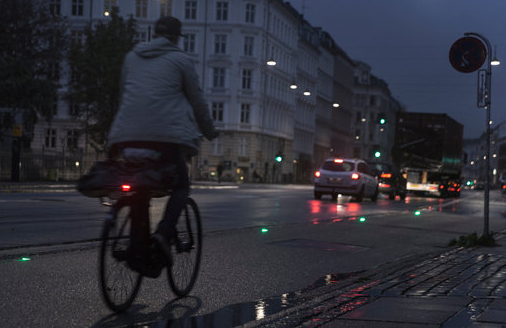
\includegraphics[width=0.7\textwidth]{copenhagen} \label{fig:copenhagen}
    \caption[Grüne Welle durch \glspl{LED}]{Kopenhagen: \glspl{LED} signalisieren die Grüne Welle bei 20 km/h  Quelle: \cite{NYT}}
\end{figure}
Zusätzlich erkennen Sensoren im Radweg Fahrradgruppen und veranlassen dann die Ampel zu einer längeren Grünphase. In einem anderen Stadtteil sind Leuchttafeln, die die verbleibende Zeit der Ampelphase anzeigen, am Radwegrand installiert\cite{KopIng}.\\
Kopenhagen als Vorbild hat Berlin mit vier Ampeln in Schöneberg eine Grüne Welle für RadfahrerInnen umgesetzt und plant bereits die zweite\cite{BZ}. Auch hier möchte man die Benutzung des Rades attraktiver machen und den Fahrradverkehr beschleunigen.
\subsection{Individuelle Ampelinformationssysteme im Auto}
In den letzten Jahrzehnten gab es immer wieder Intentionen, eine Anzeige von Geschwindigkeitsempfehlungen im Fahrzeug umzusetzen. Der folgende Abschnitt stellt existierende Lösungen und Ansätze für Ampelinformationssysteme im Auto vor.
\subsection*{Projekt Wolfsburger Welle}
Die \gls{VW}-Forschung initiierte in den 80er Jahren mit dem Projekt "'Wolfsburger Welle"' die ersten Untersuchungen zur "'Grünen Welle"' Informationen im Fahrzeug; mit der Idee, beim Annähern an eine Ampel die optimale Geschwindigkeit im Fahrzeug zu geben.\cite{Welle} "Dazu sendet die Ampelanlage ihren aktuellen Phasenzustand und eine Prognose für den nächsten Zustandwechsel an alle Fahrzeuge, die sich annähern. Der Fahrzeugcomputer setzt dann die aktuelle Fahrzeuggeschwindigkeit mit dem Abstand zur Ampel und der aktuellen Ampelphase in Bezug. Daraus wird errechnet, ob das Fahrzeug im Moment mit der grünen Welle ’mitschwimmt’ oder ob die Geschwindigkeit außerhalb des optimalen Bereichs liegt" (\cite{MenschMaschine}).
%%% TRAVOLUTION %%%
\subsection*{Projekt Travolution}
Im Sommer 2008 wurde das Projekt \textsc{Travolution} (TRAffic \& eVOLUTION), von den Projektpartnern\footnote{\cite{Travolution}} abgeschlossen. Es besteht aus den Teilprojekten \textsc{verkehrsadaptive Netzsteuerung mit Genetischen Algorithmen} und \textsc{Der informierte Fahrer}. Im Netzsteuerungsprojekt wurden 46 Lichtsignalanlagen in Ingolstadt mit der Netzsteuerungssoftware BALANCE ausgestattet, wodurch sie intelligent auf den Verkehr reagieren und die Schaltung an den Verkehr anpassen.  Ziel des zweiten Teilprojektes ist es, die Autofahrer über die Ampelphasen zu informieren. Die \gls{C2I} auf Basis von \gls{WLAN} umsetzend, senden mit Kommunikationsmodulen ausgestattete Ampeln die Grünphasen an den Bordcomputer der Autos, welcher dann die Geschwindigkeit für ein reibungsloses Passieren errechnet\cite{Stvtechnik} und wie in Abbildung \ref{fig:travolution} zu sehen ist, anzeigt. Im Rahmen des Projektes wurden zwei Anwendungsfälle umgesetzt. Die Restrotanzeige -- die die Dauer der verbleibenden Rotphase angibt, und die "'Dynamische Grüne Welle"' -- die Anzeige der Progressionsgeschwindigkeit.
Die Vorhersage der Schaltbilder ist aufgrund der verkehrsabhängigen Logik bei nicht festzeitgesteuerten \gls{LSA} nur mit einer gewissen Wahrscheinlichkeit möglich. So werden sekündlich die Grünwahrscheinlichkeiten vom \gls{LSA}-Kommunikationsmodul aktualisiert und an das Fahrzeugmodul gesendet, welches diese in Relation zu eigener Position, Geschwindigkeit und Richtung setzt und die entsprechende Empfehlung ausgibt.
\begin{figure}[H]  
    \centering  
    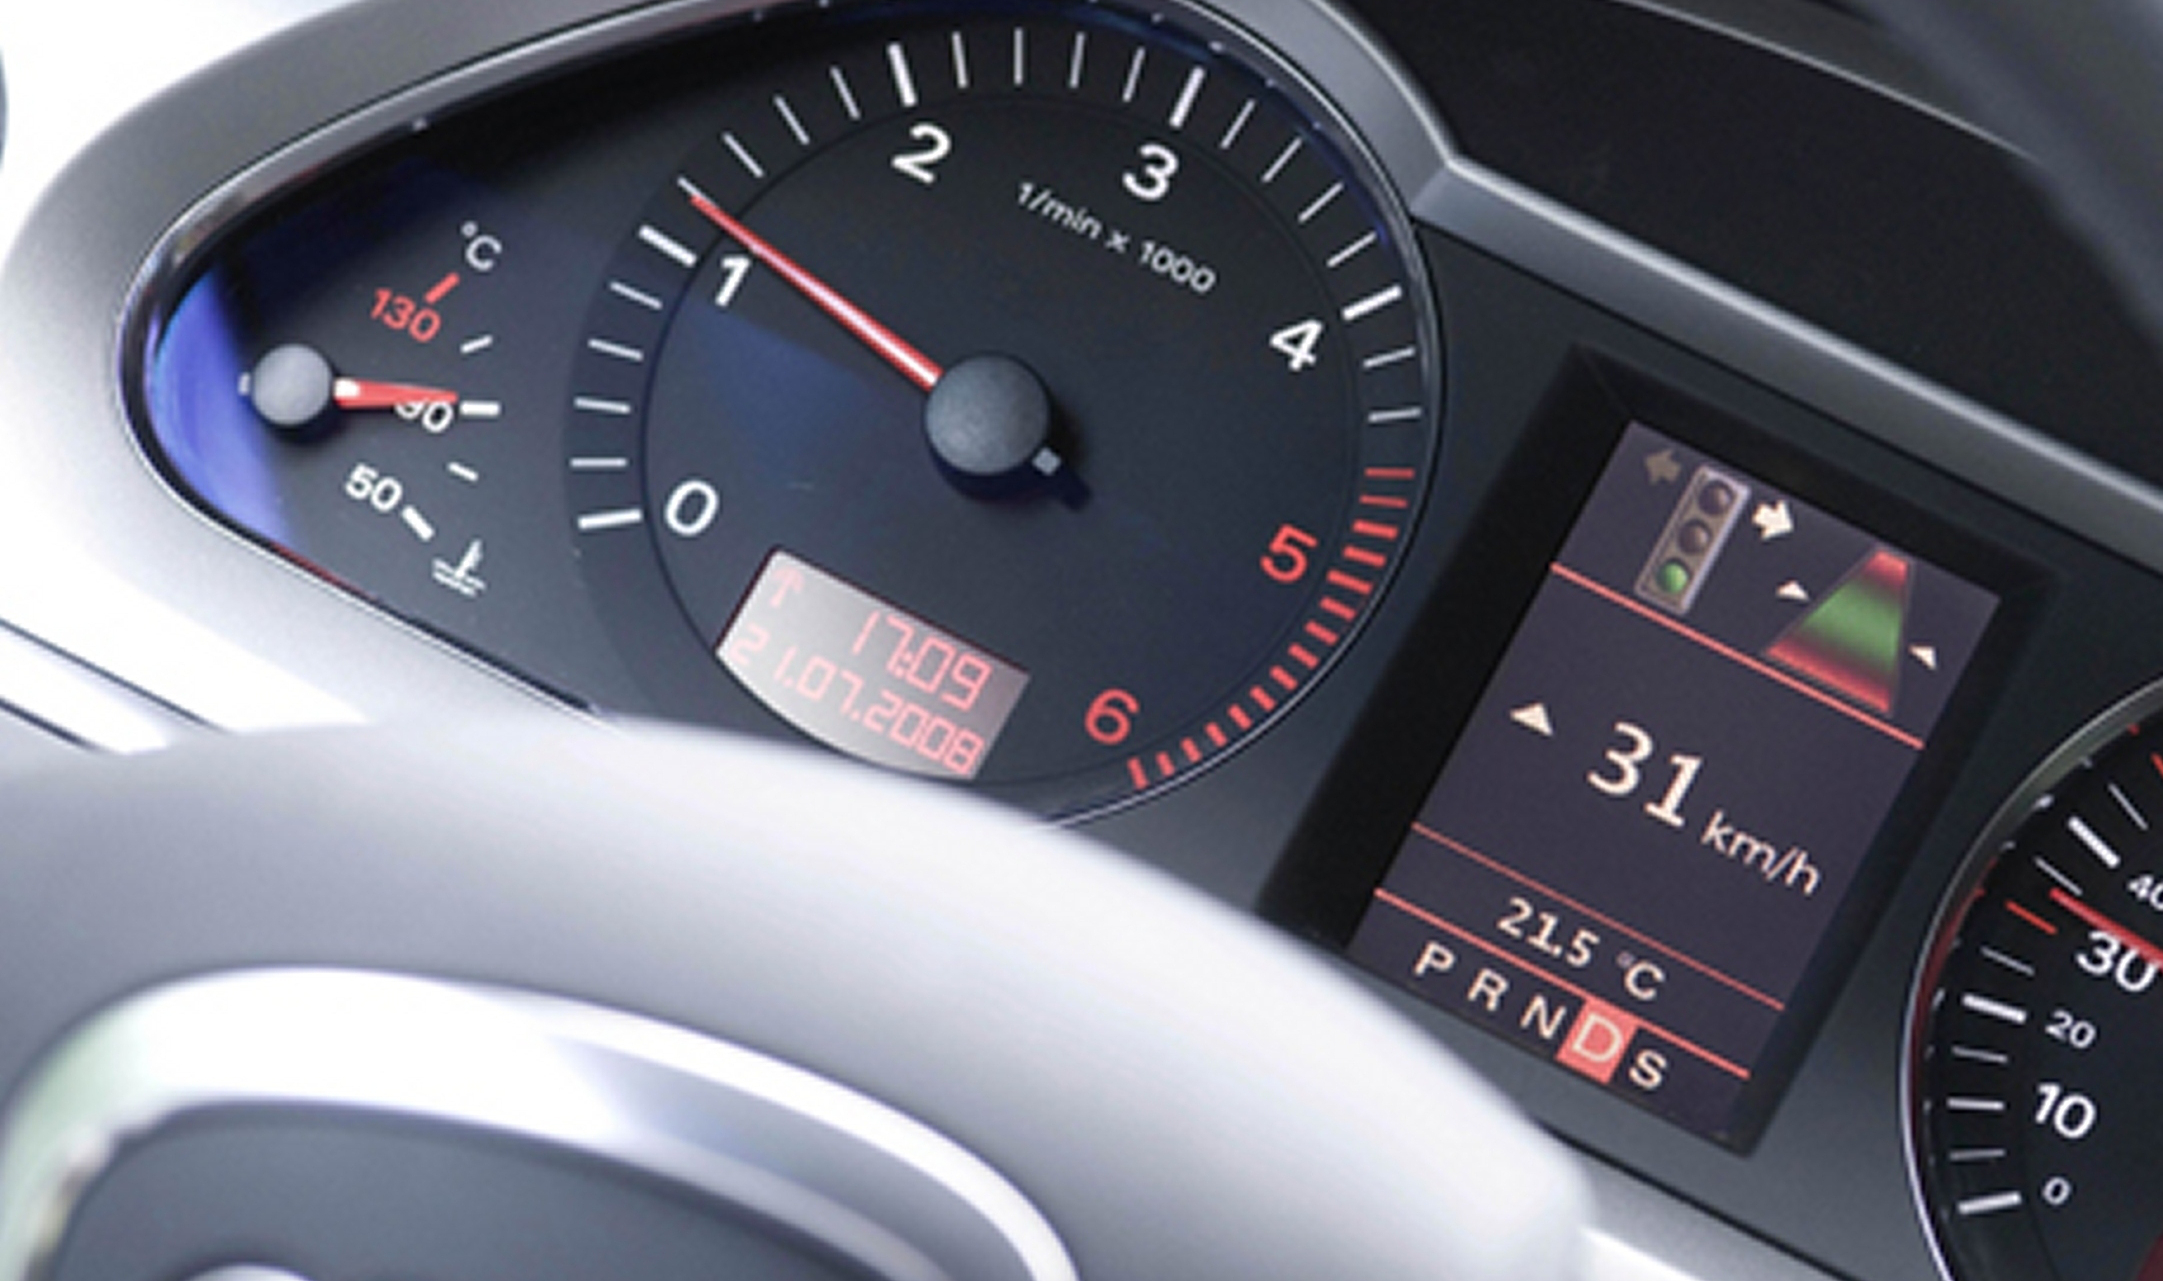
\includegraphics[width=0.7\textwidth]{travolution}      
    \caption[Projekt Travolution]{Der Bordcomputer zeigt die optimale Geschwindigkeit an. Quelle: \cite{Travolution}}
    \label{fig:travolution}
\end{figure} 
Fundierend auf \textsc{Travolution} sind Folgeprojekte wie zum Beispiel das ebenfalls von Audi ins Leben gerufene "'Ampelinfo online"' entstanden. Über Mobilfunk ist in der \gls{C2X}-Anwendung das Auto mit dem zentralen Verkehrsrechner, welcher die Ampelanlagen steuert, vernetzt und visualisiert die entsprechenden Informationen im Bordcomputer. \cite{Ampelinfo}
%%% KOLIBRI %%%
\subsection*{Projekt Kolibri}
In Bayern wurde im April 2011 das Pilot-Projekt \textsc{kolibri}\footnote{ Kooperative Lichtsignaloptimierung -- Bayrisches Pilotprojekt} mit den Teststrecken der B13 bei München mit sieben und der St2145 in der Nähe von Regensburg mit acht ampelgeregelten Kreuzungen gestartet. Gemeinsam untersuchten die Projektpartner\footnote{ \url{http://www.kolibri-projekt.de/Sites/kolibri3.html}} die Funktionen und Auswirkungen eines Ampelassistenten außerhalb von Ortschaften (\cite{kolibri}). "'Per Mobilfunk übertragen die Ampeln ihre Daten an die Zentrale der TRANSVER GmbH. Dort wertet sie ein Computer aus und sendet die Ergebnisse an die Fahrzeuge. Ein Anzeigefeld im Bordcomputer oder eine Applikation auf dem Smartphone zeigt an, ob sich das Fahrzeug in der Grünen Welle bewegt."' (\cite{kolibriTUM} ) 
\begin{figure}[H]  
    \centering  
    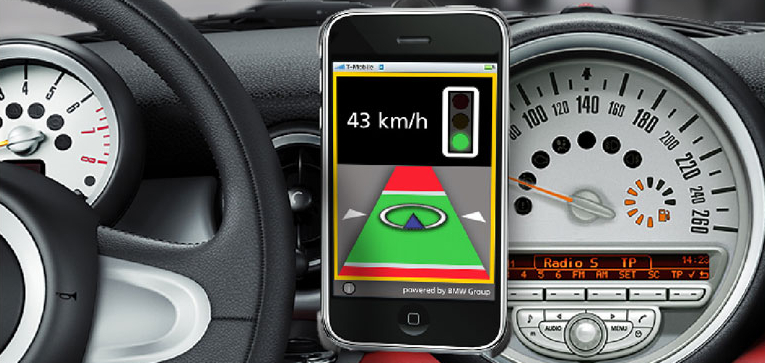
\includegraphics[width=0.7\textwidth]{kolibri}      
    \caption[Projekt Kolibri]{Anzeige der Geschwindigkeitsempfehlung. Quelle: \cite{kolibri}}
    \label{fig:kolibri}
\end{figure}
Die FahrerInnen wurden sowohl fahrzeugintegriert\footnote{ On-Board-Computer} als auch via Smartphone, wie Abbildung \ref{fig:kolibri} zeigt, über die Schaltung der nächsten Ampel informiert und erhielten Empfehlungen über die aktuelle Progressionsgeschwindigkeit. Nach zwei Jahren war das Pilotprojekt abgeschlossen 
\subsection*{Projekt Testfeld Telematik}
Ende des Jahres 2013 wurde in Wien das Projekt \textsc{Testfeld Telematik} -- Feldversuch zur Stärkung österreichischen Know-Hows im Bereich umweltverträglicher Mobilität erfolgreich abgeschlossen. Per \gls{C2X}-Kommunikation bringt das Projekt Kooperative Dienste wie Ampelinformationen direkt ins Auto. 
\begin{figure}[H]
    \centering
    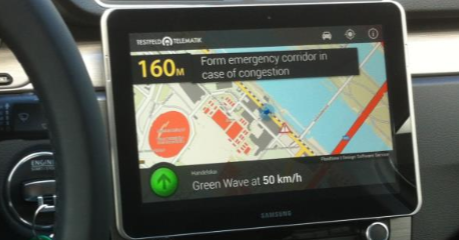
\includegraphics[width=0.7\textwidth]{telematik} \label{fig:telematik}
    \caption[Projekt Testfeld-Telematik Ampelinformation]{Mobile Anwendung des Projekts Testfeld-Telematik Quelle: \cite{Telematik}}
\end{figure} 
Über Navigationssysteme, integrierte Systeme, Nachrüst-Plattformen oder mobile Endgeräte erreicht die FahrerInnen die Information der optimalen Geschwindigkeit sowie die Dauer der jeweiligen Ampelphase\cite{Telematik}. Um an die Informationen zu kommen wurden unter anderem Kameras und Sensoren, beispielsweise als Induktionsschleife in die Fahrbahn eingelassen. Andere Autohersteller wie \gls{BMW}, Volvo und Volkswagen kooperieren als Forschungsprojekt "'Car 2 Car Communication Consortium"' mit \textsc{Testfeld Telematik}, ebenfalls mit dem Ziel die Sicherheit an Kreuzungen zu verbessern. Im Auto installierte Sensoren kommunizieren mit Kameras und Scanner in der Ampel. Allerdings funktioniert das System nur mit dem ambitionierten Ziel, wenn alle Autohersteller zusammenarbeiten und sich auf den gleichen Standard einigen. \cite{Siemens}
\subsection*{Toyota}
Auch Toyota hat ein System entwickelt, welches eine spezielle Infrastruktur an Kreuzungen, die Installation von Infrarot-Sendern, die mit dem Toyota-Navigationssystem kommunizieren erfordert. An roter Ampel werden die Fahrer über die verbleibende Wartezeit informiert. Die ausgestatteten Navigationssysteme wurden bis jetzt jedoch ausschließlich in Japan getestet. \cite{Toyota}
%
%%% Apps %%% 
%
\section{Ampelinformationssysteme als mobile Applikation}
Ampelassistenten als mobile Anwendung sind recht einfach umzusetzen. Smartphones sind bereits mit einem \gls{GPS}-Empfänger ausgestattet und haben fast durchgängig Internetzugang. Die hier vorgestellten mobilen Anwendungen existieren bereits oder befinden sich in der Testphase.
%%% ENLIGHTEN %%%
\subsection*{Mobile Applikation EnLighten}
\textsc{EnLighten} erkennt rote Ampeln und visualisiert die Dauer dieser Phase. Die mobile Anwendung nutzt \gls{GPS} zur Lokalisierung des Autos und verwendet die \gls{DSRC}-Kommunikation zu Ampelphasenprognose. An Autos und Verkehrsinfrastruktur wie Ampeln wird entsprechende Hardware installiert, die gesammelten Daten an die Verkehrszentrale gesendet, sodass dort die Ampelphasen prognostiziert werden können. Dafür werden Komponenten wie Höchstgeschwindigkeit, Ampelschaltpläne, Tageszeit und Fahrtrichtung beachtet. Mit der Verkehrszentrale verbunden, visualisiert \textsc{EnLighten} die Restrotdauer.\\ Aufgrund von hohen Installationskosten und -Aufwand ist \textsc{EnLighten} erst in einigen amerikanischen Städten funktionstüchtig und verfügbar.
%%% SIGNAL GURU %%%
\subsection*{Mobile Applikation Signal Guru}
Signal Guru wurde von den Wissenschaftlern des \gls{MIT} und der Universität von Princeton entwickelt. Die App errechnet über die Smartphones vieler Nutzer - welche miteinander kommunizieren -  die Wahrscheinlichkeit, wann eine Ampel grün wird und wie das eigene Fahrverhalten entsprechend anzupassen ist. Wie in Abbildung \ref{fig:AppSignalGuru} ist zu sehen ist, muss die eingebaute Kamera durch die Windschutzscheibe die Ampel registrieren. Bei Testläufen im Straßenverkehr vielen die Ergebnise bei statisch geschalteten Ampeln deutlich besser aus als bei angepassten Ampelschaltungen \cite{SignalGuruPaper} 
\begin{figure}[H]
    \centering
    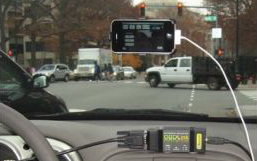
\includegraphics[width=0.7\textwidth]{SignalGuru}
    \caption[Signal Guru]{Signal Guru muss in der Lage sein die Ampel zu 'sehen'.  Quelle: \cite{SignalGuruPaper}} \label{fig:AppSignalGuru}
\end{figure}
Dieser Ansatz ist für Fahrräder jedoch nicht umsetzbar, da das Smartphone in der Halterung am Lenker die \gls{LSA} nicht erfassen kann.
\section{Fahrraderweiterungen}
Als Schnittstelle das Smarthone nutzend gibt es ausgeklügelte Systeme mit reichlich Funktionen. Das einfache Navigationssystem für Fahrräder ist kaum noch notwendig, wo doch zum Beispiel die hier aufgeführten um einiges umfangreicher sind.
\subsection{Displaylose Fahrradnavigation}
Das \textsc{Hammerhead} ist ein "'Hammer"', oder einfach ein "'T"', an den Lenker angebracht. Gespickt mit verschiedenfarbigen \glspl{LED} zeigt es den Weg zeigen, warnt vor Hindernissen und ersetzt die vorderen Scheinwerfer.
\begin{figure}[H]
    \centering
    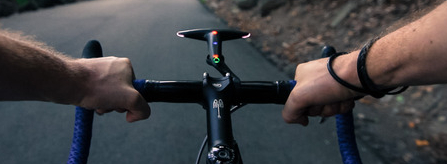
\includegraphics[width=0.7\textwidth]{hammerhead}
    \caption[Hammerhead]{Hammerhead -- \glspl{LED} zeigen den Weg.  Quelle: \cite{Hammerhead}} 
    \label{fig:hammerhead}
\end{figure}
Via Bluetooth ist \textsc{Hammerhead} an das Smartphone gekoppelt, auf dem die zugehörige Navigationsanwendung läuft mit der man Routen eingeben, teilen und speichern kann\cite{Hammerhead}.\\
Ein sehr ähnliches Prinzip verfolgt das \textsc{CycleNav} von der Firma Schwinn. Untersiede findet man hier im Design und einem integriertem Lautsprecher, der Abbiegehinweise ausgibt und auf Wunsch wiederholt\cite{CycleNav}.
\subsection{Intelligente Fahrradlenker}
Mehr High-Tech, aber auch umfangreichere Funktionen bietet der vom amerikanischen Startup \textsc{Helios-Bikes} entwickelte \textsc{Helios}-Lenker. Neben dem Frontlicht hat der Lenker wie in Abbildung \ref{fig:helios} zu sehen, an den Enden \glspl{LED} die einen zum gewünschten Standort leiten. 
\begin{figure}[H]
    \centering
    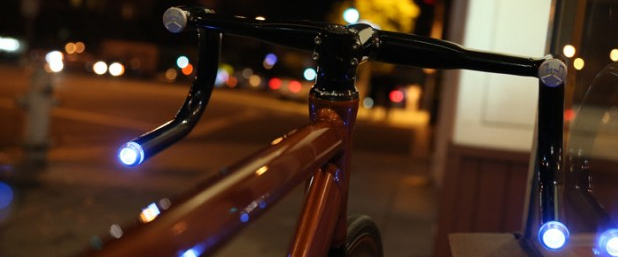
\includegraphics[width=0.7\textwidth]{helios}
    \caption[Helios-Lenker]{Helios-Lenker  Quelle: \cite{Helios}} 		
    \label{fig:helios}
\end{figure}
Sie passen ihre Farbe der Geschwindigkeit an und haben auf Wunsch auch eine Blinkfunktion. Verbindet man den Lenker mit einem Smartphone, lässt sich die Farbe der \glspl{LED} individualisieren. Die Verbindung zum Handy hat weitere Vorteile: dank des eingebauten \gls{GPS}-Trackers und eingesteckter SIM-Karte lässt sich das Fahrrad per SMS über den derzeitigen Standort abfragen\cite{Helios}, was im Falle eines Diebstahl sehr hilfreich sein kann.\\
\textsc{Vanhawks Valour} heißt das Rad, das ab April 2015 lieferbar ist. Wie im \textsc{Helios}-Lenker steckt auch hier ein über das Smartphone steuerbares Navigationssystem, das die Abbiegehinweise per \gls{LED} signalisiert, im Lenker. Auf den gefahrenen Routen merkt sich das Rad durch einen Erschütterungssensor erfasste Hindernisse wie Unebenheiten in der Fahrbahn und ermittelt beim nächsten Mal darauf rücksicht nehmend eine andere Route. Es ist darüber hinaus in der Lage mit anderen \textsc{Vanhawks valour}-Rädern zu kommunizieren und dessen Routenbegebenheiten ebenfalls zu berücksichtigen. Mittels Radarsensoren registriert das Fahrrad Autos im toten Winkel und benachrichtig die FahrerInnen durch ein vibrierenden Lenker\cite{vanhawks}.
%bluetooth kommunikation ... Akku im Rad wird mit Hilfe des Nabendynamos aufgeladen. yeah! App hat auch fitnesstrainer
\subsection{Das Samsung Smart Bike}
Auf der Mailänder Designwoche hat Samsung ein Smartbike vorgestellt, das mit verschiedenen intelligenten Komponenten wie Bluetooth, einer Kamera und Laserprojektoren ausgestattet. Der Rahmen ist aus Aluminium und leicht geschwungen, was Vibrationen abfangen soll. Wie Abbildung \ref{fig:samsung} zeigt, zeichnen vier Laserprojektoren den eigenen, begleitenden Fahrradweg auf die Straße und sollen so die Sicherheit erhöhen, indem sie den Sicherheitsabstand markieren und aus dem toten Winkel sichtbar sind. 
\begin{figure}[H]
    \centering
    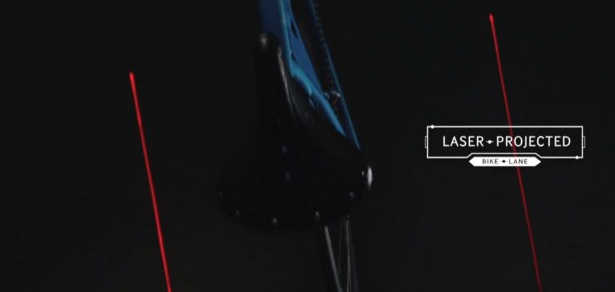
\includegraphics[width=0.7\textwidth]{samsung}
    \caption[Samsung Smart Bike]{Samsung Smart Bike  Quelle: \cite{smartbike}} 
    \label{fig:samsung}
\end{figure}
Natürlich ist auch dieses Fahrrad mit dem Smartphone verbunden, das sich dank eines Magneten einfach am Lenker anbringen lässt. Darüber kann man die Laserprojektoren ein- und ausschalten, dafür einen Timer bestimmen und über die eingebaute Kamera unter dem Sattel den Verkehr hinter sich im Auge behalten. Das Smartphone fungiert außerdem als Navigationsgerät und durch den eingebauten \gls{GPS}-Empfänger lassen eigene und Routen von anderen Nutzern speichern und intelligent verarbeiten\cite{smartbike}. Wenn also viele Menschen mit einem Samsung Smartbike unterwegs sind, erkennt das Rad die Route als angenehm und navigiert dort entlang. 
\subsection{Der COBI Fahrradcomputer}
Ein Kickstarterprojekt aus Frankfurt am Main entwickelt das System \textsc{COBI} (Connected Biking), das alle standardisierten Fahrradsysteme wie Lampen, Navigation, Tachometer etc. vereinen soll. \textsc{COBI} ist ein Modul mit inegrierter Frontleuchte in das man das Smartphone, welches dann mit der installierten \textsc{COBI}-App als Fahhradcomputer dient, legt. Durch eine wasser- und stoßfeste Hülle ist es vor Umwelteinflüssen geschützt. Zu dem Lenkersystem gibt es auch Rückstrahler die beim Bremsen intensiver leuchten und eine Blinkfunktion haben.
\begin{figure}
        \centering
        \begin{subfigure}[b]{0.49\textwidth}
                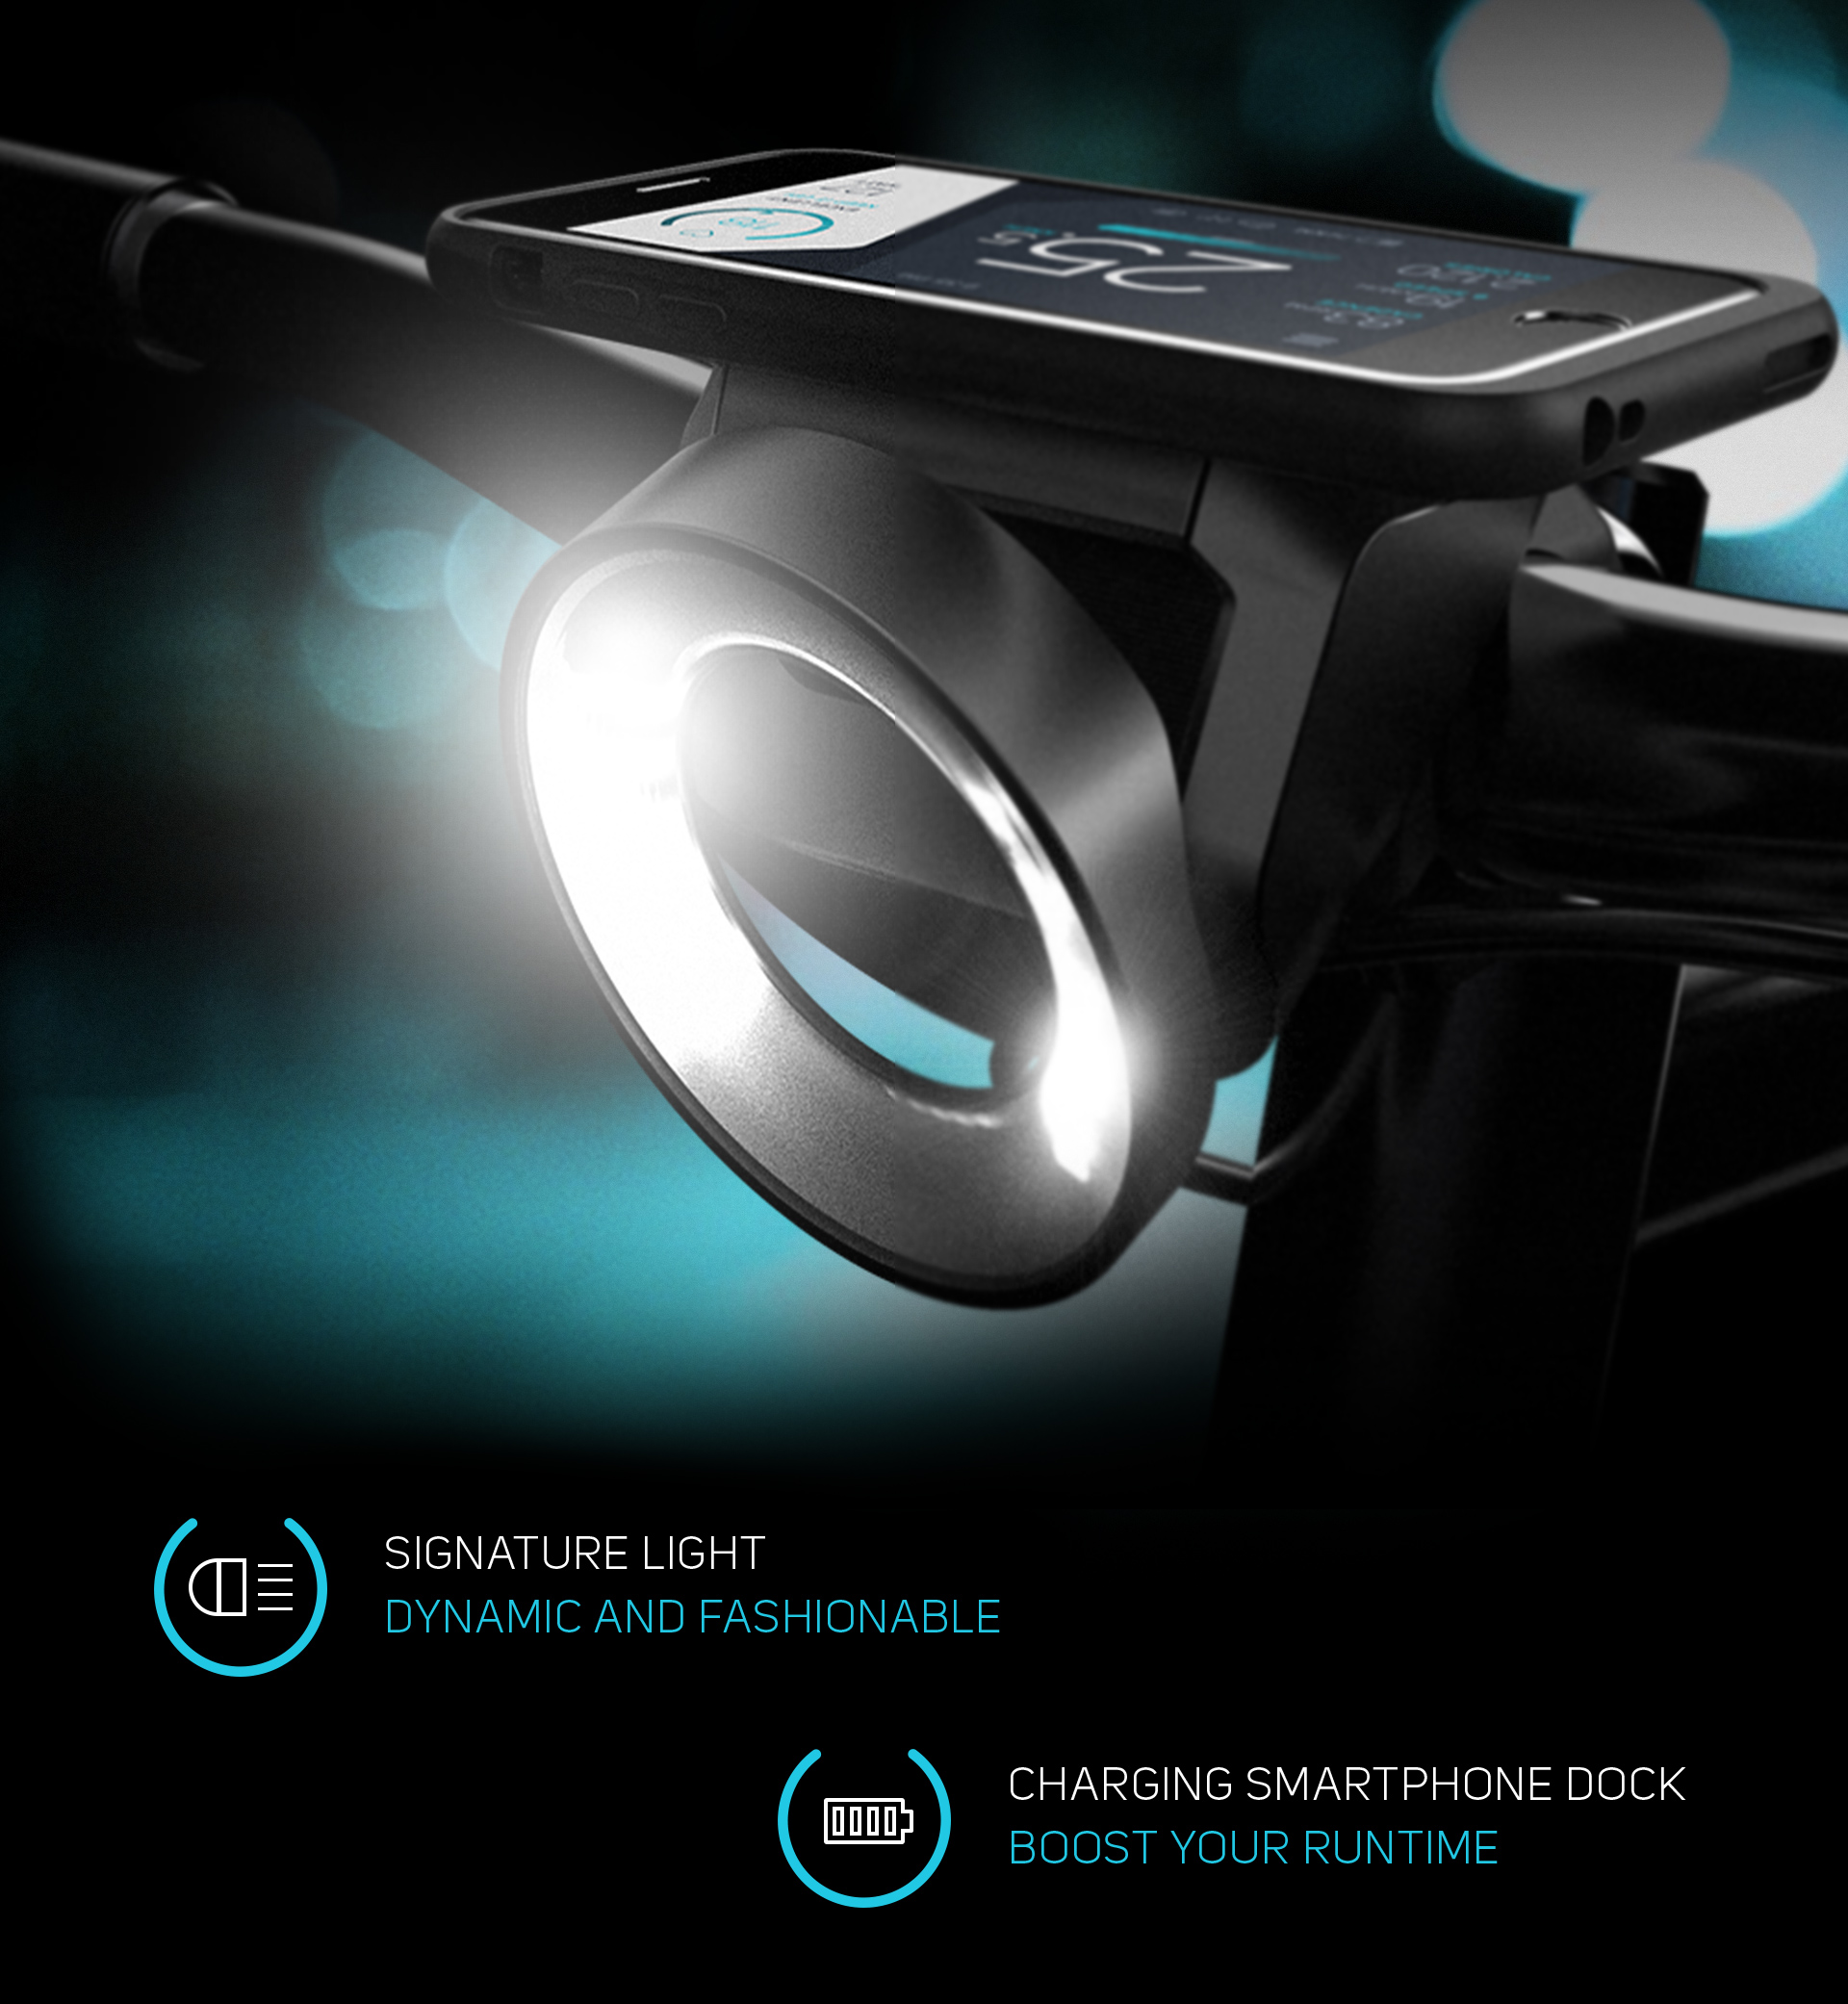
\includegraphics[width=\textwidth]{COBI_01}
                \caption{Frontlicht und Smartphonehalterung}
                \label{fig:cobi1}
        \end{subfigure}%
        ~ %add desired spacing between images, e. g. ~, \quad, \qquad, \hfill etc.
          %(or a blank line to force the subfigure onto a new line)
        \begin{subfigure}[b]{0.49\textwidth}
                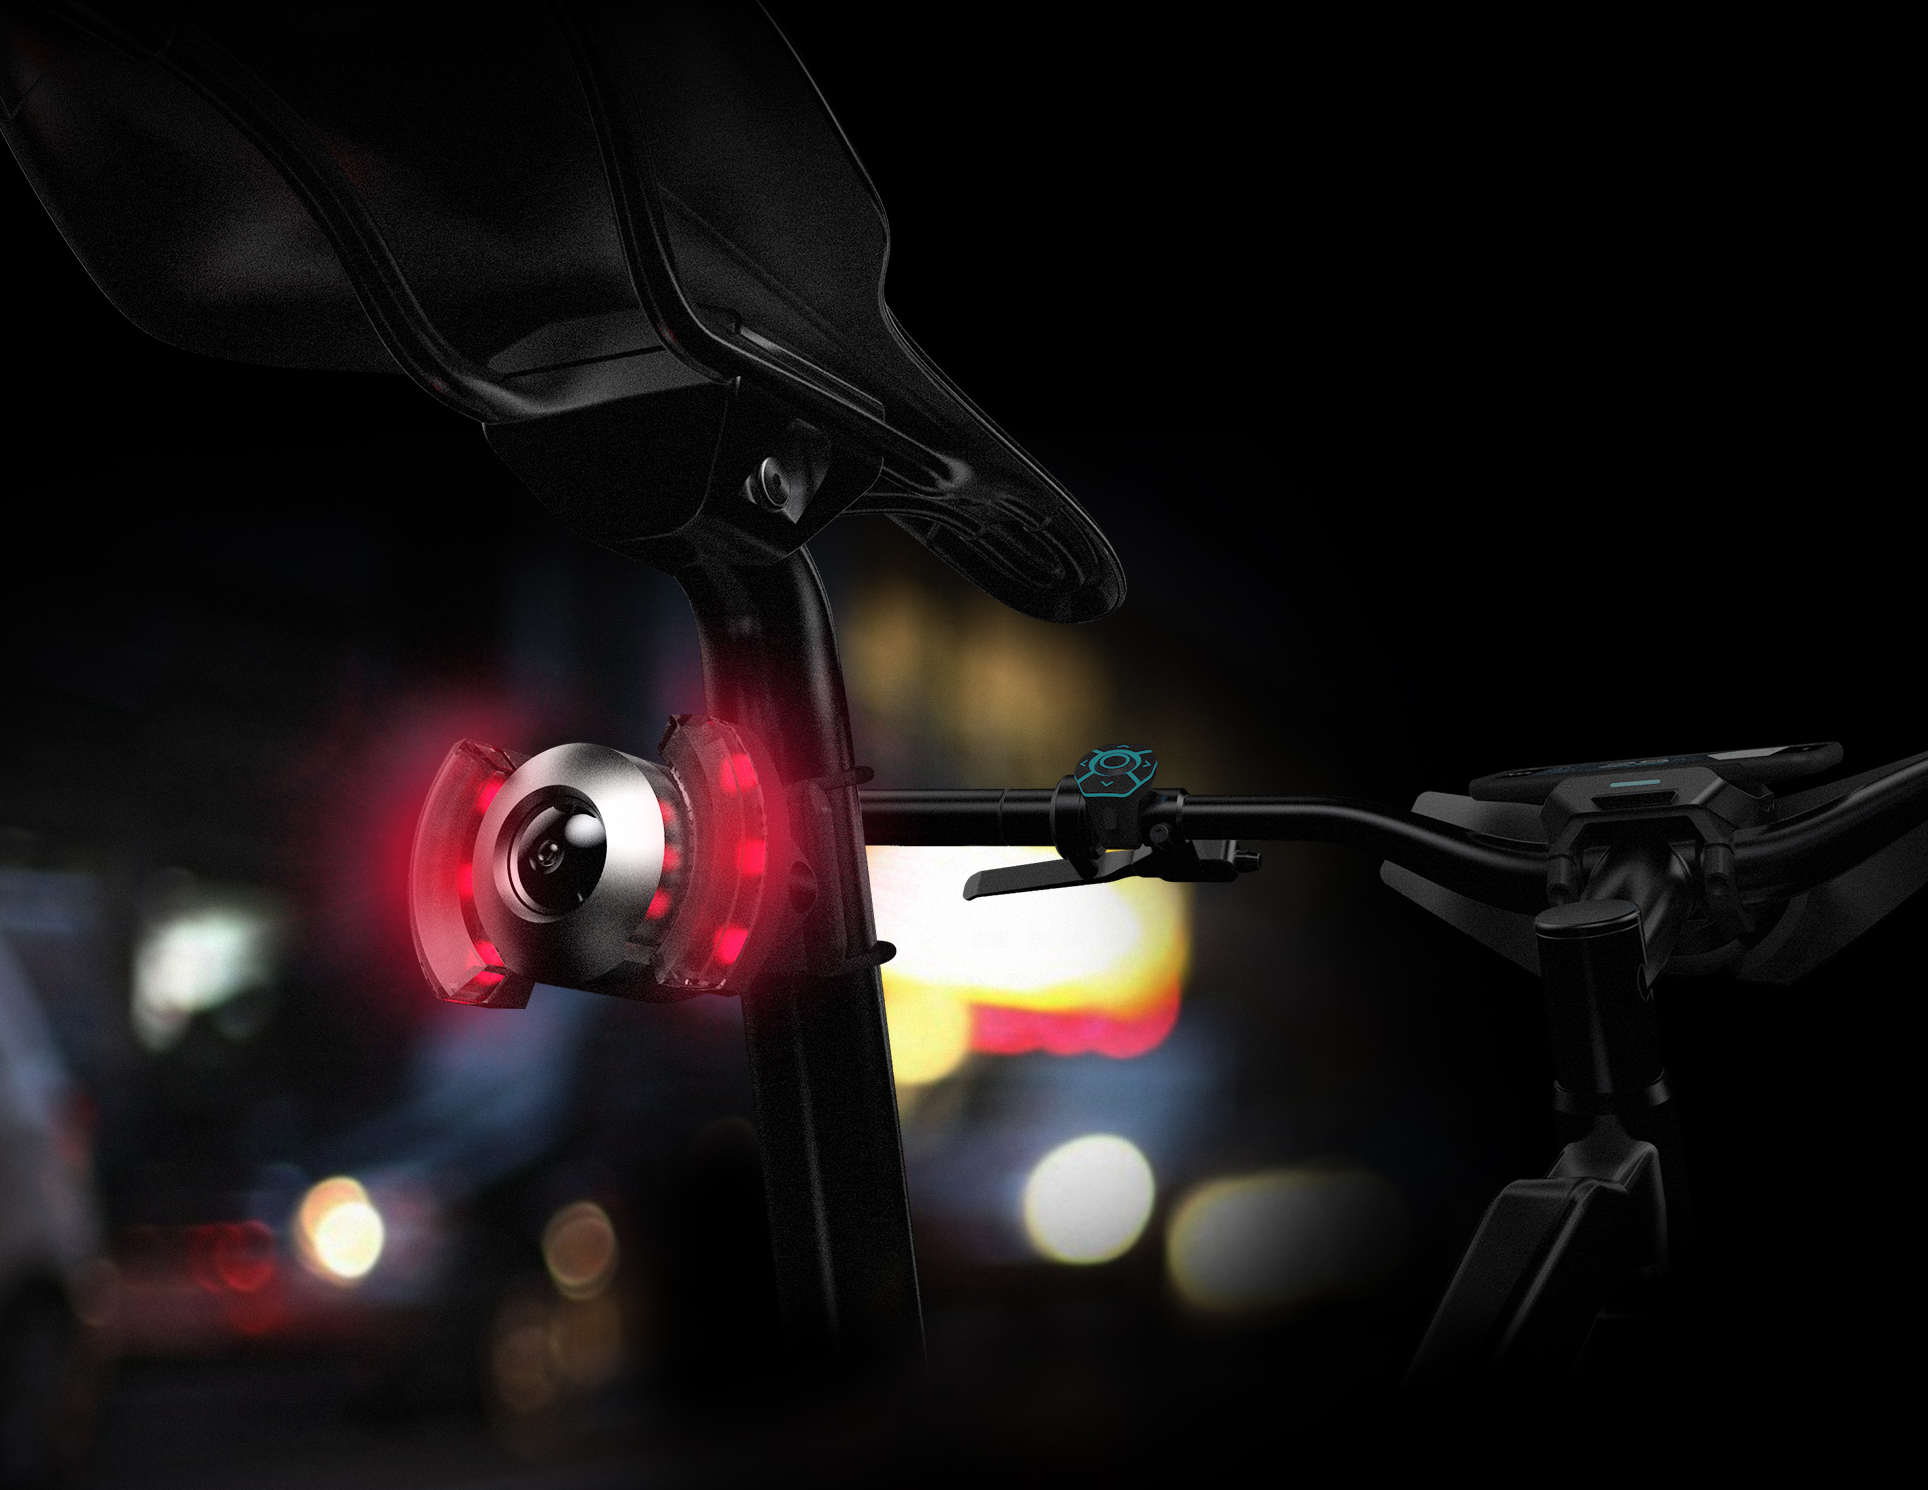
\includegraphics[width=\textwidth]{COBI_02}
                \caption{Bremslicht und Blinker}
                \label{fig:cobi2}
        \end{subfigure}
        \caption[COBI]{COBI -- Das smarte Fahrradsystem. Quelle: \cite{cobi_pic}}
        \label{fig:cobi}
\end{figure}
Möchte man das Smartphone trotzdem nicht am Lenker haben, bleibt die Verbindung zum Modul über Funk bestehen. Steuern lässt sich das System dann über einen Controller, den man am Lenker angebracht, mit dem Daumen bedienen kann. Ist es jedoch in der Halterung, wird das Smartphone über den E-Bike-Akku oder einen zusätzlich integrierten Akku aufgeladen. Wie bei den anderen genannten Systemen ist in der \textsc{COBI}-App eine Navigationsanwendung, wie auch die tracking\&share Funktion inklusive. Darüber hinaus verfügt es über einen Diebstahlschutz, Fitnesstracker sowie die Möglichkeit einer Anbindung an Spotify\footnote{ Digitaler Musikstreaming Dienst}.\\
Das Projekt ist bereits voll finanziert und der Versand der vorbestellten Systeme beginnt vorrausichtlich im Frühjahr 2015\cite{cobi}.
%%% ERGIBNIS %%%
\section{Analyseergebnis}
Diese Beispiele zeigen deutlich, dass sowohl die Nachfrage nach Ampelassistenten -- mobil oder statisch -- als auch an Fahrraderweiterungen steigt und auf dem Markt Anklang findet. Auch die EntwicklerInnen solcher Systeme werden kreativer, wodurch immer mehr Produkte mit erweiterten Funktionen entstehen. Das begeistert wiederum mehr Menschen für das Radfahren und so ist der Verkehr flüssiger, die Teilnehmer entspannter, die Luft sauberer. AutofahrerInnen sind schon lange nicht mehr allein auf der Straße und so gilt es, dieses erfolgreiche Konzept für alle VerkehrsteilnehmerInnen zu erweitern.

\chapter{\label{chap:entscheidung}Lösungsansätze}
Zur Umsetzung der beschriebenen Ampelinformationsanwendung kommen zwei Möglichkeiten in die engere Wahl. In diesem Kapitel werden die Realisierung durch eine \gls{Smartphone} \Gls{App} und die einer \gls{Arduino}-Anwendung gegenübergestellt. Zu beachten sind die Komponenten wie Sensorik, Internetverbindung, Stromversorgung und Darstellung der Informationen.\\
\begin{description}[leftmargin=0.7cm,style=nextline]
%GPS
  \item[\gls{GPS}] ~ Als Grundlage aller modernen Navigations- und Ortungssysteme im Bereich der Navigation ist \gls{GPS} für die Fahrradpositionsbestimmung obligatorisch. In einem \gls{Smartphone} ist ein \gls{GPS} Empfänger inklusive, für eine \gls{Arduino}-Anwendung ein entsprechendes Modul vonnöten\footnote{ Vgl. \cite{arduino} S. 227}.\\
 %Datenbankanbindung
 \item[Datenbankanbindung] ~ Ein weiterer wichtiger Aspekt ist die Datenbankanbindung. Mindestens die Position der Ampeln und die Phasen der Schaltpläne werden in einer Datenbankbank gespeichert und dort von der Anwendung angefragt und ausgewertet. Während man für die \gls{Arduino}-Anwendung eine Client-Server Architektur aufbauen und via Internet auf die Datenbank zugreifen muss, liefert Android die native Datenbank SQLite mit.\\
  %WWW
  \item[Internetverbindung] ~ Durch mobile Breitbandverbindung oder auch wahlweise per \gls{WLAN} ist beim \gls{Smartphone} eine Internet-Anbindung vorhanden. Das \gls{Arduino}-Board benötigt für die Netzwerkverbindung eine Erweiterung um das Ethernet-Shield. Dieses basiert auf dem Wiznet W5100 Ethernet-Chip, welcher einen Netzwerk-Stack mit UDP\footnote{ User Datagram Protocol: Netzwerkprotokoll für die verbindungslose Datenübertragung über das Internet } und TCP\footnote{ Transmission Control Protocol: Netzwerkprotokoll für bidirektionalen Datentransport} Unterstützung bietet\footnote{ Vgl. \cite{arduino} S. 36}.\\
  %STROM
  \item[Stromversorgung] ~ Die Stromversorgung ist im \gls{Smartphone} durch den integrierten Akku gegeben. Die Laufzeit ist vom Typ abhängig, genügt jedoch für die alltägliche Radstrecke. Für die mobile Stromversorgung des \gls{Arduino}-Boards wird eine 9-Volt Batterie benötigt, die zusätzlichen Platz beansprucht und wassergeschützt und gut erreichbar angebracht werden muss. Es gibt weiterhin die Möglichkeit den Strom aus dem Nabendynamo zu gewinnen. Außerdem sollte dann der \gls{Arduino} in der Lage sein Strom zu speichern, sodass die Anwendung beim Halt an der Ampel nicht ausschaltet.\\
  %DARSTELLUNG
  \item[Darstellung] ~ Ein Darstellungskonzept muss bei beiden Möglichkeiten erstellt werden. Auf dem \gls{Smartphone} ist besonders auf Erkennbarkeit bei schlechten Witterungsbedingungen, das ggf. spiegelnde Display berücksichtigend zu achten. Dafür sind aufgrund des vorhandenen Displays in gewisser Größe wesentlich mehr Informationen darstellbar. Als \gls{Arduino}-Anwendung sind lediglich ein paar helle \glspl{LED} am bzw. im Lenker erforderlich. Diese müssen doch eindeutig und intuitiv lesbar sein, um den vollen Informationsumfang zu gewähreisten.\\
\end{description}
\subsection*{Ergebnis}  
Auch wenn das Ampelinformationssystem als \gls{Arduino}-Anwendung minimalistischer ist sprechen die anderen Punkte dagegen. Beginnend bei der einfachen Stromversorgung bis hin zur vorhandenen Sensorik und internen Datenbank steht das \gls{Smartphone} weiter vorn und überzeugt durch seine Einfachheit in der Anwendung. Auch die vielen Erweiterungen die es bereits für das Fahrrad in Form einer mobilen Anwendung gibt, zeigen dass Lösungen für oben genannte Probleme wie die Nutzung bei schlechten Witterungsbedingungen existieren.

\chapter{\label{chap:grundlagen}Grundlagen}
Dieses Kapitel befasst sich mit den technischen und physikalischen Grundlagen der zu entwickelnden Anwendung.  
% -------------------------------------------------
% TECHNISCHE GRUNDLAGEN
% -------------------------------------------------
\section{\label{sec:technGrundlagen}Technische Grundlagen}
Im Rahmen dieser Arbeit wird eine \gls{Smartphone}-Anwendung erstellt, deren Implementierungsgrundlage die Software-Plattform Android und deren zentrales Merkmal die Bereitstellung von standortbezogenen Diensten ist. Die eigene Position wird mittels \gls{GPS} ermittelt, um in Verbindung mit der festen Position der nächsten \gls{LSA} die optimale Geschwindigkeit für das Erreichen der "'Grünen Welle"' zu errechnen. Im folgenden Abschnitt werden Funktionsweise und Besonderheiten der verwendeten Technologien beschrieben. 
% ANDROID
\subsection{Android}
Android ist ein von Google entwickeltes Linux-basiertes Betriebssystem für Mobilgeräte.\\ 
Android-Anwendungen werden mit der Programmiersprache Java und der Auszeichnungssprache \gls{XML} entwickelt. Mit dem Android \gls{SDK}\footnote{ Das Android \gls{SDK} steht unter \url{https://developer.android.com/sdk/index.html} zum Download bereit} werden die Werkzeuge und \glspl{API} zur Verfügung gestellt, die erforderlich sind, um Mobilanwendungen auf der Android-Plattform erzeugen zu können.\\ 
Zu den wichtigsten \gls{SDK}-Werkzeugen gehören der Android\gls{SDK} Manager, der AVD-Manager, der Emulator und der \gls{DDMS}. Der \gls{SDK} Manager verwaltet die \gls{SDK}-Pakete, sowie die installierten Pakete und System-Images. Der AVD-Manager bietet eine graphische Oberfläche, in der Android Virtuell Devices verwaltet und im Emulator ausgeführt werden können. Mithilfe des \gls{DDMS} können Android Anwendungen auf Fehler untersucht werden. \cite{android_sdk} \\\\
Mit dem Android \gls{NDK}\footnote{ Das Android \gls{NDK} steht unter \url{https://developer.android.com/tools/sdk/ndk/index.html} zum Download bereit} existiert auch eine Möglichkeit, mit dem Teile einer Anwendung in hardwarenahen Programmiersprachen wie C oder C++ implementiert werden können. Ein Programmcode, der in solchen Sprachen geschrieben ist, eignet sich zum Beispiel bei CPU-intensiven Operationen wie Signalverarbeitungen oder Physik-Simulationen besonders gut. Hier ist allerdings sicherzustellen, dass die erforderlichen Bibliotheken in dem \gls{SDK} auch verfügbar sind. \cite{android_ndk} \\
Einen Überblick über die komplexe Android-Systemarchitektur, welche nachfolgend (nach \cite{android} S. 2ff und \cite{androidVM} S.63ff) kurz beschrieben wird, zeigt die folgende Abbildung.\\
\begin{figure}[H]  
    \centering  
    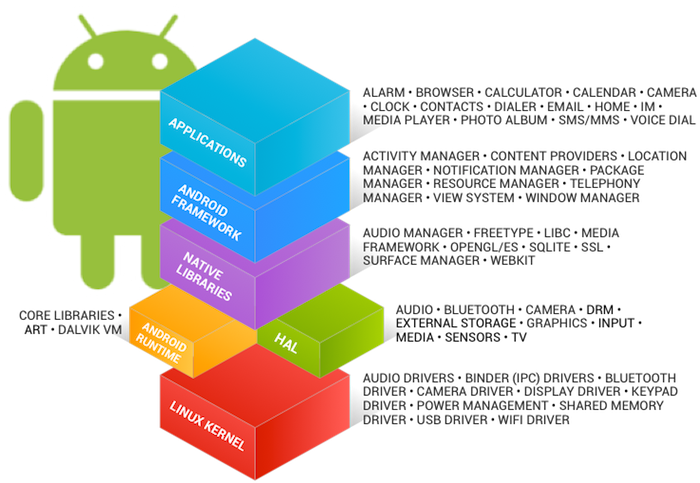
\includegraphics[width=0.8\textwidth]{android_framework_details} 
    \grayRule
    \caption[Android-Systemarchitektur]{Die Android-Systemarchitektur Quelle: \cite{android_fig}}
    \label{fig:android}
\end{figure}
\paragraph{Linux Kernel: }
Android basiert auf dem Linux-Kernel. Wie in jedem Unix-System, stellt der Kerneltreiber für Hardware, Netzwerk, Dateisystemzugriff und Prozessmanagement bereit.
\paragraph{Android Runtime: }
Die Android Laufzeitumgebung nutzt die aus dem Apache-Harmony-Projekt nachimplementierten Java-Schnittstellen, die Dalvik \gls{VM} und die mit der Version 5.0 eingeführten Android Runtime (ART). \cite{android_5}\\
Der Großteil von Android ist in Java implementiert und wird von einer \gls{JVM} ausgeführt. Androids aktuelle Umsetzung der \gls{JVM} heißt Dalvik. Dalvik wurde speziell auf mobile Geräte zugeschnitten und kann den Java-Bytecode nicht direkt ausführen. So wird der kompilierte Java-Bytecode erneut in Dalvik-Bytecode kompiliert und von der Dalvik-\gls{VM}, oder ab der Version 5.0 von der ART ausgeführt.\\
Der Hauptunterschied der beiden \glspl{VM} besteht darin, dass ART die binäre Maschinensprache bei der \gls{App}-Installation, und nicht wie die Dalvik-\gls{VM}, bei der Ausführung erstellt.
\paragraph{\gls{HAL}: }
Der \gls{HAL} bietet die Möglichkeit, eigene Gerätespezifikationen und deren benötigte Treiber, verbunden über eine Software-Schnittstelle zwischen dem Android-Stack und der Hardware, zu implementieren. \cite{android_hal}
\paragraph{Bibliotheken: }
Systemeigene Bibliotheken sind C/C++ Bibliotheken und diese sind vorinstalliert. Dazu gehören alle Bibliotheken im lilanen Bereich von Abbildung \ref{fig:android}:
\begin{itemize}[leftmargin=0.7cm]
\renewcommand\labelitemi{--}
	\item \textsc{Surface Manager}: ~ Der für die Displayverwaltung verantwortliche Oberflächen-Manager
	\item \textsc{OpenGL/ES}: ~ Eine 2D und 3D -Grafikbibliothek
	\item \textsc{SGL}: ~ Eine 2D-Grafikbibliothek
 	\item \textsc{Media-Framework}: ~ Eine Medien-Bibliothek zur Wiedergabe von Audio- und Video-Daten 	
 	\item \textsc{FreeType}: ~ Eine Bibliothek zur Darstellung von Computerschriften als Rastergrafik
 	\item \textsc{SSL}: ~ Das Secure-Socket-Layer für die Internet-Sicherheit
	\item \textsc{SQLite}: ~ Eine ausgereifte Datenbank die den internen Gerätespeicher nutzt 
	\item \textsc{Webkit}: ~ WebKit ist die Standard-Browser-Engine und erlaubt das Rendern und Anzeigen von HTML Seiten
	\item \textsc{libc}: ~ Eine C-Bibliothek mit Basisfunktion
\end{itemize}
\paragraph{Application Framework: }
Androids Application-Framework ist eine Umgebung, die unterschiedliche Dienste zur Verfügung stellt. Sie bietet EntwicklerInnen Zugriff auf die im Kern verwendeten \glspl{API} sowie auf die Java-Bibliotheken, die für Android erstellt wurden. 
\paragraph{Applications: }
Auf der obersten Ebene in Abbildung \ref{fig:android} befinden sich die Anwendungen, die den täglichen Telefon-Bedarf wie Adressbuch, Media-Player, E-Mail, Internet-Browser etc. decken. Zusätzlich unterstützt Android verschiedene Anwendungen von Drittanbietern.
%
% MOBILE SENSING
%
\subsection{Mobile Sensorik} 
Ein Sensor\footnote{ aus dem Lateinischen, deutsch: "'\textit{fühlen}"'} ist ein Bauelement, das physikalische Eigenschaften wie Helligkeit, Temperatur oder Beschleunigung sowohl quantitativ als auch qualitativ erfassen und in ein analoges Signal umwandeln kann. \cite{sensor} \\\\
%\textit{Nahezu alle aktuellen \glspl{Smartphone} enthalten einen \gls{GPS}-Sensor, über denn der jeweilige Standort ermittelt wird. Im nächsten Abschnitt wird auch darauf eingegangen, wie Weiterhin können zur Ortsbestimmung Daten aus Funkzellen und naheliegender kabelloser Netzwerke hinzugezogen werden.}
% % MOBILE SENSORIK UNTER ANDROID %
%\subsubsection{Mobile Sensorik unter Android}
Die meisten Android-Mobilgeräte verfügen über integrierte Sensoren, die die Bewegung, Ausrichtung und verschiedene Umgebungsbedingungen messen. Diese Sensoren sind nützlich, wenn man dreidimensionale Gerätbewegungen, Positionierungen oder Änderungen in der Umgebung des Gerätes überwachen möchte. So können zum Beispiel Spieleanwendungen den Beschleunigungssensor nutzen, um komplexe BenutzerInnengesten und Bewegungen wie Neigung, Erschütterung, Drehung oder Schwenkung zu erfassen.\\
Die Android-Plattform unterstützt Bewegungssensoren zum Messen von Beschleunigungen und Drehungen in drei Achsen, Umgebungssensoren zur Ermittlung verschiedener Umweltparameter wie Luftdruck und -feuchtigkeit, Beleuchtung, Temperatur sowie Positionssensoren zum Messen der physikalischen Ausrichtung des Gerätes. Android bietet mit dem Android Sensor Framework eine Sammlung von Klassen und Schnittstellen, mit deren Hilfe man auf diese Sensoren zugreifen und deren Daten erfassen kann. \cite{android_sensor}  
%
% LOCATION BASED SERVICE
%
\subsection{Standortbezogene Dienste}
Standortbezogene Dienste (\gls{LBS}) sind Informationsdienste, die die geographische Position des Endgeräts nutzen, um für die NutzerInnen einen Mehrwert bereitzustellen. Sie ermöglichen den NutzerInnen, den eigenen Standort zu bestimmen, zu erfahren was sich in der Nähe befindet und dieses (z.B. in sozialen Netzwerken) zu bewerten. Für die Bereitstellung von \gls{LBS} sind die vier Schlüsselkomponenten Mobilgerät, Content-Provider, Kommunikationsnetzwerke und Lokalisierungstechniken erforderlich. Das Kommunikationsnetzwerk (z.B. Internet) übeträgt die Daten an den Content-Provider (z.B. Server), welcher die bearbeiteten Anfragen an das Mobilgerät sendet (vgl. \cite{gps} S. 4f).\\
Zur Bestimmung von Standortdaten gibt es mehrere Lokalisierungstechniken. Einige davon werden im Folgenden erklärt.
%
% GEOLOKATION NETWORK PROVIDER %
%
\subsubsection{Standortbestimmung via Netzwerk}
Netzwerkgestützte Standortbestimmung basiert auf Informationen des \glspl{WLAN} oder der Funkzellen des Mobilfunknetzes.\\ 
% MOBILFUNK %
Funkzellentriangulierung verwendet die bekannte Geschwindigkeit von Funksignalen, um den Abstand zum Empfangsgerät zu berechnen. Das Mobilgerät muss mit einem Funkturm in Verbindung stehen. Bewegt sich das Gerät, verbindet es sich mit einem anderen Turm und die Signalstärke des sich nähernden Turms wird stärker. Unter Kenntnis der eindeutigen ID sowie der Position des Funkturms, mit dem das Gerät verbunden ist und ggf. der Funktürme, mit denen das Gerät zuletzt verbunden war, lässt sich der eigene Standort ermitteln (vgl. \cite{location} S. 8f). \\
Für eine gute Lokalisierung braucht es mindestens drei, vorzugsweise vier Mobilfunkmasten oder Antennen. In Städten, wenn sich mehr Signale der Mobilfunkmasten überlappen, kann eine Genauigkeit von bis zu 200 Metern erreicht werden -- bei einer geringen Funkturmdichte kann diese auf mehreren Kilometer sinken, wie in Abbildung \ref{fig:cell3} illustriert. \\
Eine Überlappung von den Signalen dreier Funktürme ist in Abbildung \ref{fig:cell1} veranschaulicht. Diese Genauigkeit kann, wie in Abbildung \ref{fig:cell2} demonstriert, erhöht werden, wenn Richtantennen auf dem Funkturm installiert sind. So kann zusätzlich die Richtung des Mobiltelefonsignals ermittelt werden (vgl. \cite{gps} S. 23). \\
\begin{figure}[H]
        \centering
        \begin{subfigure}[t]{0.23\textwidth}
                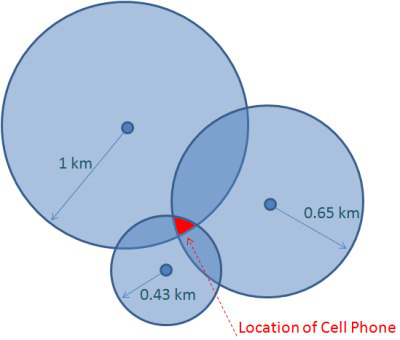
\includegraphics[width=\textwidth]{triangulation1}
                \caption{Überlappung von Signalen dreier Funktürme}
                \label{fig:cell1}
        \end{subfigure}
        ~ 
        \begin{subfigure}[t]{0.23\textwidth}
                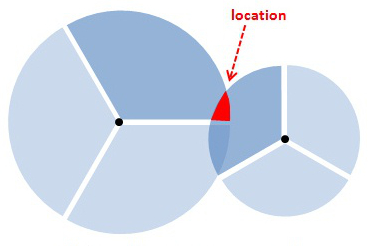
\includegraphics[width=\textwidth]{triangulation2}
                \caption{Überlappung von zwei Funktürmen mit Richtantennen}
                \label{fig:cell2}
        \end{subfigure}
         ~ 
        \begin{subfigure}[t]{0.23\textwidth}
                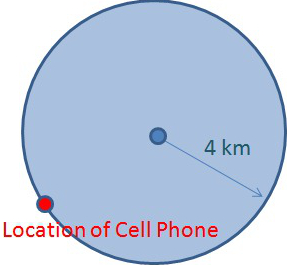
\includegraphics[width=\textwidth]{triangulation3}
                \caption{Keine Überlappung von Funkturmsignalen}
                \label{fig:cell3}
        \end{subfigure}
        \grayRule
        \caption[Funkzellentriangulierung]{Funkzellentriangulierung Quelle: \cite{fig:cell}}
        \label{fig:cell}
\end{figure}
%Ähnlich der funkzellenbastierten Standorterkennung funktioniert die \gls{WLAN}-basierte.
\gls{WLAN}-basierte Standorterkennung funktioniert durch Funksignale, die von \gls{WLAN}-Access Points\footnote{ Drahtloser Zugangspunkt, der als Schnittstelle für kabellose Kommunikationsgeräte dient} ausgesendet werden, um den genauen Standort eines jeden Wi-Fi-fähigen Gerätes zu ermitteln. Bei Aktivierung scannt die Software die Umgebung nach \gls{WLAN}-Access Points und berechnet die Position des Gerätes, indem sie die empfangenen Signale mit der Referenzdatenbank vergleicht. Wie bei der funkzellenbastierten Standorterkennung erhöht sich auch hier die Genauigkeit (auf 20 bis 40 Meter in Europa) mit wachsender Signaldichte. \\
Effektiv werden die gleichen Prinzipien der Funkzellentriangulation übernommen. Nur werden WiFi-SSIDs\footnote{ Service Set Identifer (SSID), Service Set bezeichnet alle Geräte in einem \gls{WLAN}, welche dann durch die ID ansprechbar werden} statt Funkzellenidentifikationsnummern zum Feststellen der Sendequellen verwendet (vgl. \cite{gps} S. 32ff). \\
Netzwerkgestützte Standortbestimmung schont zwar im Gegensatz zu \gls{GPS} den Akku und ist innerhalb von Gebäuden nutzbar, liefert jedoch wesentlich ungenauere Ergebnisse.
% GEOLIKATION GPS %
\subsubsection{Standortbestimmung via \gls{GPS}}
Die satellitengestützte Positionsbestimmung \gls{GPS} gewährleistet die Bestimmung des exakten Standpunktes und ist so wesentlicher Bestandteil ortsgebundener Anwendungen wie zum Beispiel der in Kapitel \ref{chap:state} beschriebenen. \\
\gls{GPS} wurde ursprünglich vom US-Militär entwickelt und dann Mitte der 90er Jahre der Öffentlichkeit zur Verfügung gestellt. Noch heute bleibt es mit einer Genauigkeit von bis zu drei Metern die genaueste Lokalisierungstechnologie (vgl. \cite{gps} S. 24f).\\
Das Globale Positionsbestimmungssystem umfasst 27 Satelliten, die ständig die Erde umkreisen und dabei kontinuierlich ihre eigene, aktuelle Position und Almanach-Daten aussenden. Almanach-Daten enthalten Daten über jeden Satelliten in der Konstellation. Abbildung \ref{fig:gps} zeigt eine Darstellung der GPS-Satellitenkonstellation. Jeder Satellit folgt einer definierten Bahn, sodass mindestens vier Satelliten von jedem Standpunkt von der Erde aus "'sichtbar"' sind (vgl. \cite{location} S. 4f).\\
Mittels Triangulation errechnet daraus ein \gls{GPS}-Empfänger die eigene Position. Mit den Daten eines einzigen Satelliten lässt sich die Position des \gls{GPS}-Empfängers auf einen großen Bereich der Erdoberfläche einschränken. Das Hinzufügen eines zweiten engt die Position auf den Bereich, in dem sich die beiden Teilbereiche überlappen ein. Mit den Daten eines dritten Satelliten bekommt man bereits eine relativ genaue Positionierung. Mit jedem weiteren Satelliten wird die Präzision erhöht und durch zusätzliche Positionsinformationen, wie z.B. Höhe über dem Meeresspiegel, erweitert. \gls{GPS}-Empfänger benutzen normalerweise vier bis sieben, oder gar mehr Satelliten (vgl. \cite{gps} S. 25f).\\
\begin{figure}[H]  
    \centering  
    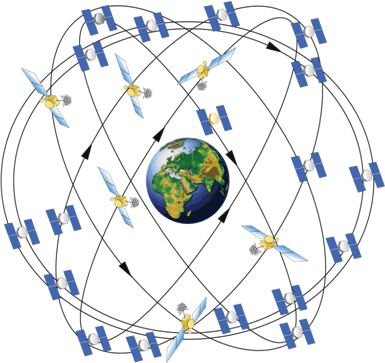
\includegraphics[width=0.4\textwidth]{gps} 
    \grayRule
    \caption[GPS-Satelliten-Konstellation]{GPS Satelliten Konstellation  Quelle: \cite{fig:gps}}
    \label{fig:gps}
\end{figure}
Trotzdem hat \gls{GPS}, insbesondere für mobile Plattformen einige Nachteile. Es verbraucht relativ viel Energie, was die Akkulaufzeit des Mobiltelefons beeinträchtigt. Bevor der jeweilige Standort berechnet werden kann, müssen mehrere Satelliten ermittelt werden, was nach dem Kaltstart\footnote{ Start ohne aktuelle Satellitendaten} einige Zeit in Anspruch nehmen kann (vgl. \cite{location} S. 5).\\\\
Inzwischen wird auf einigen Mobiltelefonen zusätzlich das russische \gls{GNSS} names \glstext{GLONASS}\footnote{ GLONASS, russisch Globalnaja nawigazionnaja sputnikowaja sistema, dt. Globales Satellitennavigationssystem} eingesetzt\footnote{ z.B. in Sony Mobiltelefonen. Siehe hierzu: \url{http://developer.sonymobile.com/2012/01/19/glonass-support-in-our-latest-xperia-phones/ -- Zugriff: 12.03.20}}.
Die europäische Variante in der Testphase mit ähnlichem Aufbau heißt Galileo, das chinesische (ausschließlich in China nutzbar) \gls{GNSS} heißt BeiDou\footnote{ BeiDou, dt. Großer Bär} (vgl. \cite{gps} S. 24).
% A-GPS
\subsubsection{\gls{A-GPS}}
Viele moderne \glspl{Smartphone} sind heutzutage mit der \gls{GPS}-Variante \gls{A-GPS} ausgestattet. Hierbei werden Zusatzinformationen über die nächstgelegenen Satelliten via Mobilfunk bezogen, sodass die Erstbestimmung der Position sehr viel schneller ablaufen kann.
Voraussetzung hierfür ist die Ausstattung der Mobilfunktürme mit \gls{GPS}-Empfängern, welche kontinuierlich die Satellitenpositionen beziehen. Diese Daten werden, sobald angefordert, an das Mobiltelefon gesendet (vgl. \cite{gps} S. 26f). \\
\gls{A-GPS} benötigt daher nur die Sicht auf einen Satelliten und erzielt durch die Einbeziehung der Assistenzinformationen trotzdem genauere Ergebnisse in der Ortsbestimmung.
Dieses ist insbesondere in Städten (Einschränkung des \gls{GPS} durch z.B. hohe Gebäude) von Vorteil.
% GEOLOLATION UNTER ANDROID %
\subsubsection{Standortbestimmung unter Android}
Android unterstützt mit dem \texttt{android.location} Paket den Zugriff auf die Ortungsdienste. Als zentrale Komponente des Location Frameworks stellt der \texttt{LocationManager} \glspl{API} zur Lokalisierung des Geräts bereit. Mit dem \texttt{LocationManager} ist die Anwendung in der Lage, alle Location Provider\footnote{ Location Provider, dt. Standortanbieter. Ein Standortanbieter bietet regelmäßige Berichte über die geographische Lage des Gerätes} des letzten bekannten Standortes abzufragen, sich für regelmäßige Updates zur Position des Gerätes anzumelden und sich wieder abzumelden, wenn sich das Gerät außerhalb gegebener Parameter befindet. \cite{android_gps} \\
Die geographische Positionsangabe besteht aus Längengrad (Latitude) und Breitengrad (Longitude). Beide werden unter anderem vom \texttt{LocationManager} über das \texttt{Location}-Objekt als Gleitkommawert geliefert. Daneben auch Informationen wie die Höhe in Metern über der Meereshöhe, Peilung, Zeitstempel und die Geschwindigkeit.\\
Der Abstand zwischen zwei Punkten kann mit \texttt{Location.distanceBetween()} abgerufen werden. Diese Methode bekommt als Parameter die Längen- und Breitenkoordinaten der beiden Punkte und ein Array mit \texttt{float}-Werten für die Ergebnisse übergeben. Dieses Array muss eine Größe von mindestens eins haben und gibt die ungefähre Entfernung in Metern im Index Null zurück. Abstandsberechnungen werden mit dem Referenzsystem WGS84\footnote{ World Geodetic System}-Ellipsoid definiert (vgl. \cite{location} S.43). 
\\\\
Der Fused Location Provider verwaltet die zugrunde liegenden Ortungstechnologie. Er ermöglicht zum Beispiel den Zugriff auf die letzte Position und minimiert den Energieverbrauch der Anwendung, indem er auf Grundlage aller eingehenden Standortanfragen und verfügbaren Sensoren die effizientesten auswählt. \cite{android_fused}
\clearpage
% -------------------------------------------------
% MATHEMATISCHE GRUNDLAGEN
% -------------------------------------------------
\section{\label{sec:mathGrundlagen}Berechnungsgrundlagen der Geschwindigkeitsempfehlung}
Präsentiert das System während der Anwendung eine Geschwindigkeitsempfehlung, ist diese abhängig von der aktuellen Fahrgeschwindigkeit und vom Abstand zur Ampel. Für einen Streckenabschnitt $s$ zwischen zwei Punkten (Position der Ampel und Position der Rades) wird die Zeitspanne $\Delta t$ benötigt. Diese errechnet man mit $t_{2} - t_{1}$. In Kenntnis dieser beiden Größen lässt sich dann die erforderliche Durchschnittsgeschwindigkeit im untersuchten Streckenabschnitt errechnen.\\\\ 
Angenommen die \gls{Progressionsgeschwindigkeit} $v$ wird zum Zeitpunkt $t_{1}$ ermittelt, die \gls {LSA} schaltet zum Zeitpunt $t_{2}$ auf Rot und Abstand zur Ampel beträgt $s$, dann gilt: \\
\[ v = \frac{s}{t_{2} - t_{1}} \] \\
Die aus den erfassten Daten erstellten Ampelsignalpläne und Position der angesteuerten Ampel sind die Basis dieser Berechnung. Die aktuelle Position des Fahrrads wird vom \gls{GNSS}-Sensor des \glspl{Smartphone} ermittelt und daraus der Abstand zur Ampel errechnet. Die Abbildung \ref{fig:vst} illustriert die Grundlagen der Geschwindigkeitsberechnung: \\
\begin{figure}[H]  
    \centering  
    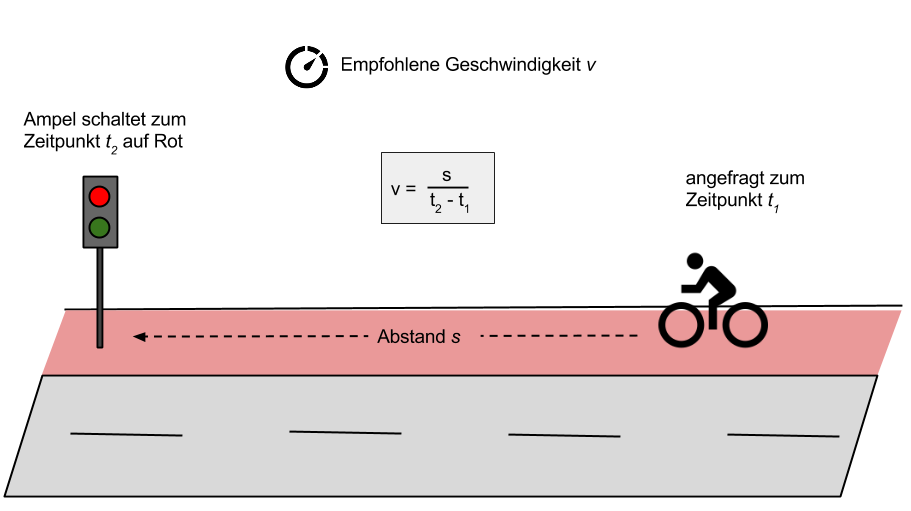
\includegraphics[width=\textwidth]{vst}  
    \grayRule
    \caption[Berechnung \gls{Progressionsgeschwindigkeit}]{Visualisierung der Geschwindigkeitsberechnung}
    \label{fig:vst}
\end{figure}
\clearpage
Da das System für Fahrräder entwickelt wird, ist auch die maximal mögliche Beschleunigung von Bedeutung. FahrradfahrerInnen können nicht unbegrenzt beschleunigen, um die gewünschte Geschwindigkeit zu erreichen. Sie ist abhängig von der Geschwindigkeit und der Zeitspanne, in der diese zu erreichen ist. Die Formel für Beschleunigung lautet:
\[ a = \frac{v}{(t_{2} - t_{1})^{2}} \]\\
 Um die ensprechende \gls{LSA} während der Grünphase zu passieren, muss letztendlich die empfohlene Geschwindigkeit $v$ eingehalten werden, wobei die maximal mögliche Beschleunigung $a$ nicht überschritten werden kann.

\chapter{\label{chap:szenarien}Szenarien im Ampelbereich}
Alle in Kapitel \ref{chap:state} angeführten Studien zu Ampelinformationssystemen und Konzepte zu Fahrraderweiterungen haben die Gemeinsamkeit des selbstkontrontollierten Fahrverhaltens der FahrerInnen. Ausgesprochen werden lediglich Empfehlungen, die möglichst intuitiv und schnell vermittelt werden. Grundlegend sollte die Anwendung in der Lage sein, die passende Empfehlung oder Handlungsaufforderung anzuzeigen, die sich aus folgenden Szenarien ergeben.
\begin{figure}[H]  
    \centering  
    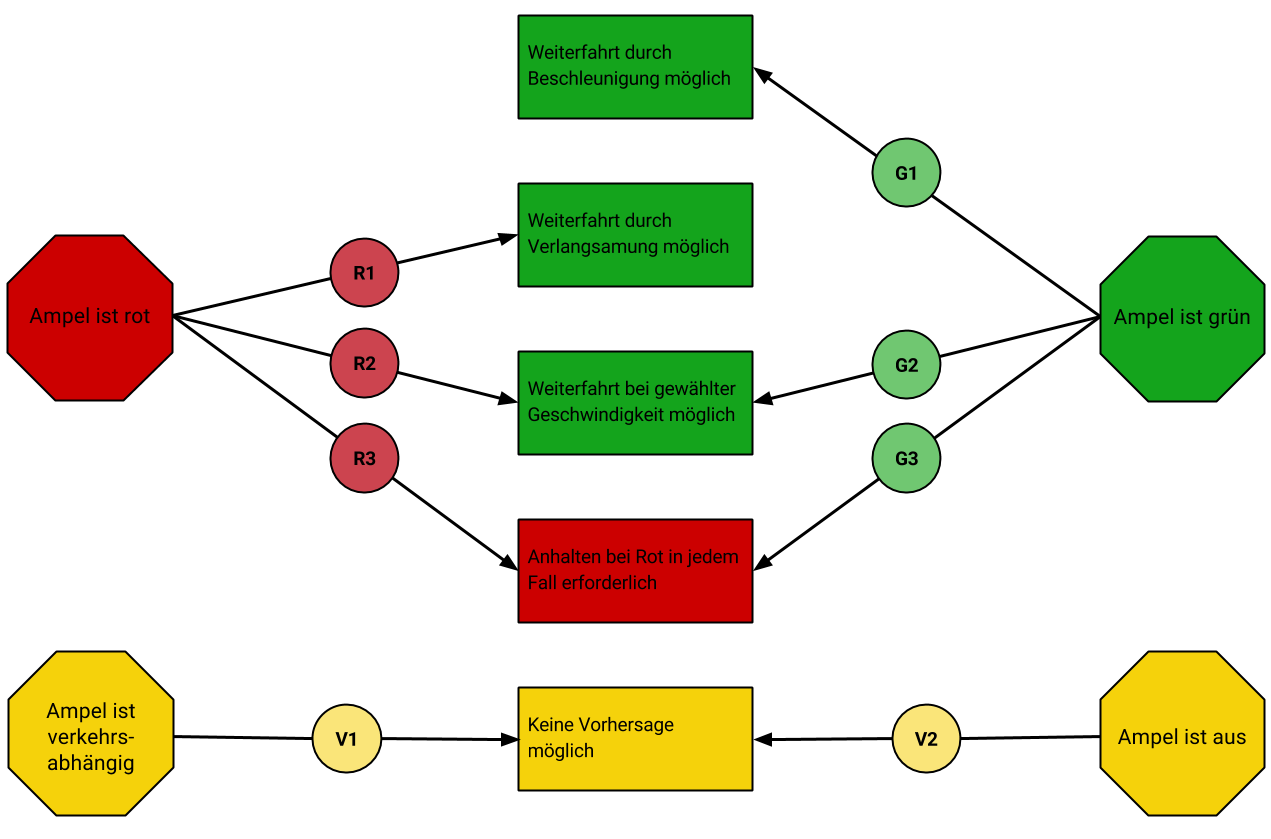
\includegraphics[width=1\textwidth]{Szenarien} 
    \caption[Szenarien]{Szenarien im Ampelbereich}
    \label{fig:szenarien}
\end{figure}
\begin{description}[leftmargin=0.7cm,style=nextline]
\item[Szenario R1:] 
Zeigt die Ampel im Moment und noch eine ganze Weile auf Rot ist je nach Distanz zwischen Ampel und Fahrrad ist ein reibungsloses Passieren der Ampel durch Beschleunigung oder ohne Änderung der Geschwindigkeit zu erreichen.\\
\item[Szenario R2:] 
Die Ampel zeigt im Moment auf Rot, aber die Restrotzeit ist kurz. Auch hier gilt: Je nach Entfernung zwischen Fahrrad und \gls{LSA}, ist ein reibungsloses Passieren der Ampel durch Verlangsamung oder ohne Änderung des Tempos zu erreichen.\\
\item[Szenario R3:] 
Zeigt die Ampel im Moment Rot, die Restrotzeit ist lang, doch die Entfernung zwischen Fahrrad und \gls{LSA} hoch, so ist keine Weiterfahrt ohne Unterbrechung möglich.\\
\item[Szenario G1:] Ist die empfohlene Geschwindigkeit gleich der aktuellen, ist ein reibungsloses Passieren bei beibehaltenem Tempo möglich. Es besteht kein Aktionsbedarf.\\
\item[Szenario G2:] 
Zeigt die Ampel im Moment Grün und ist die empfohlene Geschwindigkeit höher als die aktuelle, ist ein reibungsloses Passieren durch Beschleunigung zu erreichen. Bei der Anzeige der Progressionsgeschwindigkeit ist selbstverständlich die geltende Höchstgeschwindigkeitsbegrenzung oder die eingestellte Höchsteschwindigkeit zu beachten.\\ 
\item[Szenario G3:] 
Zeigt die Ampel im Moment Grün und ist die empfohlene Geschwindigkeit höher als die aktuelle und gleichzeitig auch höher als die zugelassene, bzw. eingestellte Höchstgeschwindigkeit, ist die Distanz zur Ampel zu groß und ein reibungsloses Passieren nicht möglich.
\end{description}
Resultierend aus den Szenarien im Ampelbereich ergeben sich die folgenden Systemzustände.
Weiterfahrt ohne Aktion möglich, Weiterfahrt durch Beschleunigung möglich, Weiterfahrt duch Verlangsamung möglich und keine Weiterfahrt ohne Unterbrechung möglich. Im weiteren Verlauf wird beschrieben wie diese Systemzustände in ein Designkonzept eingebunden werden.

\chapter{\label{chap:anforderungen}Anforderungsdefinition}
Dieses Kapitel soll helfen eine Vorstellung für die Anforderungen an die Ampelhinweis -App zu bekommen. Im heutigen High-Technologie Zeitalter spielt die Benutzbarkeit und Funktionalität des Produkts eine große Rolle. Es geht nicht nur darum, Interesse zu wecken, sondern auch die NutzerInnen für das Produkt zu begeistern. \\
Aus den oben genannten Szenarien werden im Folgenden die Anforderungen hergeleitet, die die zu entwickelnde \gls{Smartphone}-Anwendung erfüllen soll. Für die Umsetzung einer solchen Applikation ist die Positions- und Geschwindigkeitsbestimmung obligatorisch. Im Zusammenhang mit den Ampeldaten, bestehend aus Lage- und Schaltplan sollen die notwendigen Berechnungen durchgeführt und deren Ergebnisse als Empfehlung ausgesprochen.
% FUNKTIONALITÄT %
\section{Funktionalität}
Die Bestimmung der Position, Fahrtrichtung und Geschwindigkeit des Fahrrads ist die zentrale Voraussetzung für eine zeitgerechte Empfehlung. Sie sollte ebenso schnell wie präzise erfolgen, sodass keine Verzögerung der berechneten Ergebnisanzeige eintritt und die Informationen eine hohe Genauigkeit betragen.\\
Von ebenso hoher Relevanz sind die Ampeldaten bestehend aus der genauen Position der \gls{LSA} und deren Schaltpläne. Es muss ermittelt werden, welche Ampel die nächste ist und daraus die Entfernung zu dieser berechnen. 
\textit{Da nicht alle \gls{LSA} in Berlin automatisch geschaltet sind, sondern einige verkehrsabhängig gesteuert werden -- wie zum Beispiel FußgängerInnenampeln, die erst auf Druck aktiviert werden -- ist es nicht möglich für diese eine genaue Vorhersage zu treffen. Wird die nächstgelegene Ampel als solche identifiziert, muss die Anwendung sofort signalisieren, dass keine Empfehlung zu erwarten ist. Ebenso unbeachtet bleiben zunächst die Linksabbieger-Ampeln die auf die Hauptampel folgen. Da zuerst die Hauptampel passiert werden muss und die Linksabbieger-Ampel versetzt zu dieser geschaltet ist, ist beim Abbiegewunsch das Anhalten unvermeidbar.}
\subsection{Berechnungen}
Abschnitt \ref{sec:mathGrundlagen} legt die Berechnungsgrundlagen hierfür dar. Die ausgesprochene Empfehlung basiert auf der berechneten Empfehlungsgeschwindigkeit, welche abhängig vom Abstand zu Ampel und der aktuellen Geschwindigkeit ist. Der Abstand zur Ampel wird durch die verbleibende Zeit, bis die Ampel umschaltet, dividert um die Progressionsgeschwindigkeit zu erhalten.\\\\
Die Berechnung bedarf sinnvoller Geschwindigkeitsparameter. Wenn man zu langsam fährt, ist es schwer den Lenker gerade zu halten oder man fällt irgendwann vom Rad. Demnach Ist eine Untergrenze von 5km/h festzulegen. Die Obergrenze richtet sich in erster Linie nach der zulässigen Höchstgeschwindigkeit. Denn auch wenn Fahrräder nicht von den allgemeinen Geschwindigkeitsbegrenzungen der StVO nach \S 3 Abs. 3 der StVO betroffen sind, gelten per \S 3 Abs. 1 der StVO die per Schild angeordneten Geschwindigkeiten. Eine Höchstgeschwindigkeit von 30 km/h soll als Ausgangspunkt für die zu implementierende Anwendung dienen. Gegebenenfalls kann diese später individuell angepasst werden. \\
Wird die berechnete Geschwindigkeit mit der aktuellen und den Begrenzungsparametern ins Verhältnis gesetzt, ist die Empfehlung abzuleiten. Die Prognose findet statt, sobald die Ampel circa 300 Meter voraus liegt. Bei einer größeren Entfernung von zum Beispiel einem Kilometer kann die Gefahr der Ablenkung bestehen. Sollte die Anwendung auf der Strecke durchgängig vorschlagen schneller zu fahren, könnte die fahrende Person dies als Ansporn sehen und so nicht mehr auf den Verkehr achten. Bei dieser doch recht kurzen Entfernung genügt für den zu entwickelnden Prototyp der Abstand als Berechnungsbestandteil in Luftlinie. Bei Optimierungsbedarf bietet es sich hierfür an, Kartenmaterial einzubinden, um den genauen Abstand ermitteln zu können. Hierbei werden dann beeinflussende Elemente wie Hügel oder Kurven berücksichtigt.
\subsection{Positionsdaten}
Die Positionsdaten und Schaltpläne, im Uhrzeit- oder Datumsformat befinden sich in einer Datenbank. Die von Android bereitgestellte systemeigene Datenbank SQLite nutzt den internen Speicher des Geräts und ermöglicht so einen schnellen Zugriff auf diese Daten. Die Datenbank wird als Datei in der Anwendung abgelegt, wodurch sich Abfragen zu externen Servern, die eine Verbindung mit einem Netzwerk voraussetzen erübrigen. Diese sollte allein aus Performancegründen keinen Internetzugriff voraussetzen, da ein direkter Zugriff auf den internen Speicher nicht den Umweg über einen Server gehen muss. Ist das Datenvolumen aufgebraucht, ist die Netzwerkverbindung zu langsam die benötigsten Daten zeitnah anzufragen und zu erhalten.\\\\
Trotz des erhöhten Stromverbrauchs bei der Verwendung von \gls{GPS} ist es von Vorteil auf die netzwerkgestützte Standortbestimmung zu verzichten, da die Genauigkeit dieser Verfahren nicht so präzise ist. 
\textit{Eine Möglichkeit dem hohen Akkuverbrauch von \gls{GPS} entgegenzuwirken wäre die Verwendung eines externen \gls{GPS}-Geräts, das über Bluetooth mit dem \gls{Smartphone} verbunden ist und so dessen Akkulaufzeit verlängert. Außerdem ist die Qualität des \gls{GPS}-Empfängers höher als die des im \gls{Smartphone} verbauten und kann somit eine präziesere Ortung erlangen. (Vgl. \cite{gps} S. 28) Der Nachteil hierbei ist die Notwendigkeit eines zweiten Gerätes.} 
% DESIGN %
\clearpage
\section{Die graphische Oberfläche}
Ebenso wie die Bestimmung der Position und Geschwindigkeit spielt auch die graphische Darstellung eine große Rolle. Gerade bei dem Gebrauch im Verkehr ist die Eindeutigkeit und schnelle Erfassbarkeit der zu übermittelnden Informationen bedeutend.  \\
Um nicht von dem Verkehr abzulenken muss die Information, sowohl in Bedeutung als auch in Darstellung auf einen kurzen Blick erkennbar sein. Demnach sollte die Oberfläche möglichst einfach gehalten werden.\\
Da die Anwendung während der Fahrt nicht bedienbar sein muss -- denn auch das würde vom Verkehr ablenken -- besteht mehr Raum für die Informationsanzeige. 
Es ist davon auszugehen, dass die Anwendung ausschließlich im Freien Gebrauch findet. Dies und die dort herrschenden wechselnden Helligkeiten, zum Beispiel bei der Fahrt durch Schatten, setzen eine Verwendung von hohen Kontrasten voraus.
\subsection{Empfehlungsanzeige}
Im Allgemeinen sollte die Anwendung in der Lage sein die sich aus Kapitel \ref{chap:szenarien} resultierenden vier Systemzustände zu visualisieren und gegebenenfalls eine entsprechende Empfehlung auszusprechen.\\
Zur Verdeutlichung und einfacher Erfassbarkeit bietet es sich an, die entsprechenden Farben zu nehmen. Also ist für Zustand \textit{b}, der das Erreichen der Grünen Welle ohne Veränderung der eigenen Geschwindigkeit steht Grün und für den Zustand \textit{a}, der ausdrückt dass keine Weiterfahrt ohne an roter Ampel Anhalten zu müssen möglich ist, Rot zu verwenden.
Die Zustände \textit{c} und \textit{d} drücken aus, ein Erreichen der Grünen Welle ist möglich, jedoch nur bei Veränderung der eigenen Fahrgeschwindigkeit. Zur inhaltlichen Differenzierung ist eine andere Farbe zu wählen, sodass bereits aus dem Augenwinkel erkennbar ist "'Ich muss etwas tun"'. Dahingehend soll ersichtlich sein, wieviel getan werden muss. Sprich die Anwendung soll zwischen zwei Graden unterscheiden können: ob das Tempo leicht oder stark erhöht bzw. verlangsamt werden muss. Wird die Empfehlung der leichten Geschwindigkeitverlangsamung ausgesprochen, muss auch das ersichtlich sein.\\
Unterstützend zur Handlungsaufforderung kann ein Countdown angezeigt werden, der die Dauer der jeweiligen Ampelhase herunterzählt. 
   
\chapter{\label{chap:entwurf}Konzeption}
Die erarbeiteten Anforderungen an ein Ampelinformationssystem für FahrradfahrerInnen werden in diesem Kapitel für die Konzeption angewendet. Beginnend mit dem Aufbau der Anwendung werden in den folgenden Abschnitten das Design, die von der Anwendung genutzten Daten, Anwendungsfälle, die Architektur und schließlich die Komponenten der Entwicklumgsumgebung, welche eingesetzt werden aufgeführt. 
\section{Anwendungsaufbau}
Die Anwendungsarchitektur verwendet die Vorgaben für Android-Applikationen. So wird die Hauptkomponente mit Hilfe sogenannter \glspl{Activity} realisiert. Als Basisklasse definiert eine \gls{Activity} das \gls{UI} einer mobilen Anwendung, stellt also die Ansicht mit der BenutzerInnen interagieren können bereit.\\
Eine \gls{Activity} wird von der Bibliotheksklasse \texttt{android.app.Activity} abgeleitet, als Klasse implementiert und muss in der Manifestdatei der \gls{App} aufgeführt werden. \cite{android_activity} \\
In der zu entwickelnden Fahrradapplikation wird keine Navigation innerhalb der Anwendung vonnöten sein, weshalb nur eine \gls{Activity} implementiert wird.
% DATENGRUNDLAGE
\section{Datengrundlage}
%Ampeldaten werden erstellt. eigene Positionsdaten werden ermittelt,... 
Zur Umsetzung der Anwendung werden die Ampeldaten benötigt, welche dann im \gls{JSON}-Format als Datei auf dem Mobilgerät abgelegt werden müssen.
\subsection{Ampeldaten}
\textit{... Um einen Überblick zu gewähren, werden jedoch die wichtigsten Komponenten skizziert.\\ 
Jede Kreuzung hat bis zu vier Schaltpläne, die zu festgelegten Tageszeitabschnitten greifen. Tabelle \ref{tab:zeitplan} zeigt, wie der Tagesplan einer Kreuzung aussehen kann, wobei an anderen Tagen die Uhrzeiten sowie die Reihenfolge und Quantität der Zeitschaltprogramme variieren können:}
\begin{figure}[H]
\centering
	\begin{minipage}[b]{0.29\textwidth}	
		\raisebox{\depth}{\begin{tabular}{@{}cc@{}}
			\toprule
			\rowcolor[HTML]{ECF4FF} 
			\multicolumn{2}{l}{\cellcolor[HTML]{ECF4FF}\textsc{\centering \large Bezeichnung der Kreuzung}}                                                                  \\ \midrule
			\rowcolor[HTML]{EFEFEF} 
			\multicolumn{1}{l}{\cellcolor[HTML]{EFEFEF}\textbf{Uhrzeit}} & \multicolumn{1}{l}{\cellcolor[HTML]{EFEFEF}\textbf{Schaltprogramm}} \\ \midrule
05:00 & Tag   \\ \midrule
08:30 & Früh  \\ \midrule
14:00 & Spät  \\ \midrule
19:00 & Tag   \\ \midrule
00:01 & Nacht \\ \bottomrule
		\end{tabular}}
		\captionof{table}{Zeitschaltplan}	
		\label{tab:zeitplan}
	\end{minipage} \hfill
%
	\begin{minipage}[b]{0.6\textwidth}
		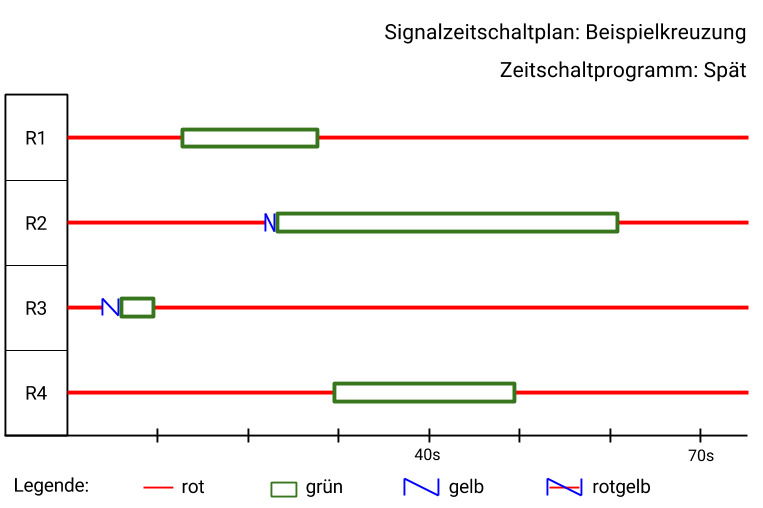
\includegraphics[width=\textwidth]{szpl}
		\subcaption[Signalplan]{Typischer Signalschaltplan einer Ampel  Quelle: \cite{fig:signal}}
		\label{fig:plan}
	\end{minipage}
	\rule{35em}{0.5pt}
	\caption{Beispielschaltpläne vierer Ampeln einer Kreuzung}	
\end{figure}
\textit{Für jedes Schaltzeitprogramm existieren ein Schaltzeit- und für einige Kreuzungen ein bis zwei Alternativschaltzeitpläne die in Intervallen von 60 bis 90 Sekunden die Rot-, Grün, Gelb, Rotgelb und Dunkelphasen zeigen. In den Dunkelphasen ist die \gls{LSA} ausgeschaltet -- zur Anschaltung gibt es dann den entsprechenden Einschaltplan. Abbildung \ref{fig:plan} zeigt auf, wie so ein Schaltzeitplan für eine Kreuzung aussehen kann. Um die Ampel dem entsprechenden Schaltplan zuzuordnen, liegen Lagepläne als \gls{PDF}-Datei bei, die eine genaue Darstellung der Kreuzung mit all ihren Komponenten zeigt. }
\begin{figure}[H]  
    \centering  
    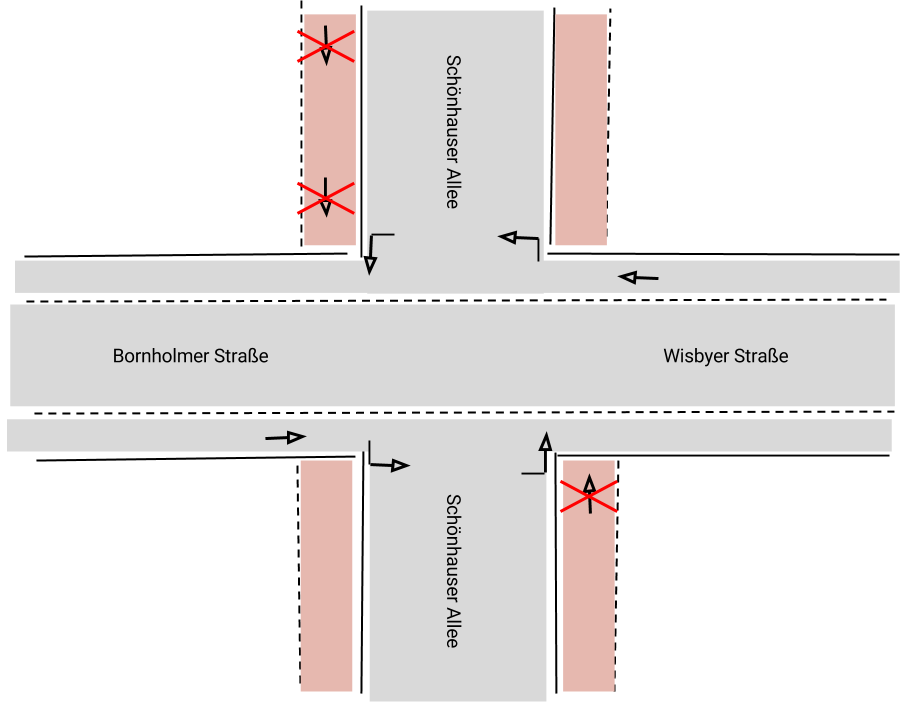
\includegraphics[width=0.7\textwidth]{kreuzung} 
    \rule{35em}{0.5pt}
    \caption{Lageplan}
    \label{fig:kreuzung}
\end{figure}
\textit{Da die Position der Ampeln als Lageplan vorliegen, }sind diese manuell in das WGS84-Format konvertiert und in das gewählte \gls{JSON}-Format gebracht werden.
Als Referenzzeit ist die Zeit zwischen 14 und 20 Uhr von Montag bis Freitag gewählt. Diese kann selbstverständlich bei Bedarf ausgedehnt bis vervollständigt werden.
%
% LSA als JSON
%
\subsection[Ampelobjekt im JSON-Format]{Ampelobjekt im \gls{JSON}-Format}
\gls{JSON} ist ein leichtgewichtiges, auf JavaScript basierendes, Datenaustauschformat, das für Menschen gut les- und schreibbar und für Maschinen einfach analysier- und generierbar ist. Ein \gls{JSON}-Objekt besteht aus einer von zwei Grundstrukturen. Eine Auflistung von Schlüssel/Wert Paaren oder eine geordnete Liste von Werten, als Array realisiert. Der folgende Codeabschnitt zeigt beispielhaft ein \gls{JSON}-Ampelobjekt:  
\begin{center}
\rule{35em}{0.5pt}
\lstinputlisting[language=JSON, caption=JSON-Ampelobjekt]{code/lsas.json}
\rule{35em}{0.5pt}
\end{center}
Das hier aufgeführte Ampelobjekt hat den Namen \texttt{SteinstraßeA1}, welcher auf die Kreuzung auf der sich die Ampel befindet schließen lässt. Es folgen die zwei Werte \texttt{lat} und \texttt{lon}, die die genaue Position der \gls{LSA} beschreiben und der boolsche Wert \texttt{dependsOnTraffic}, der auf \texttt{false} gesetzt ist, sobald die Ampel verkehrsunabhängig ist. Im anderen Fall ist sie verkehrsabhängig und fällt somit aus den Berechnungen heraus, benötigt also auch keine weiteren Daten. Das Array \texttt{timetable} beinhaltet Schaltplanobjekte mit einem Array aus Tagen und der Start-und Endzeiten an denen diese gelten. Die Werte \texttt{greenFrom} und \texttt{greenTo} bezeichnen den Start und das Ende jeder Grünphase des Schaltplans. Da als Referenzzeit die Zeit zwischen 14 und 20 Uhr gewählt wurde, werden die Schaltpläne, welche diese nicht betreffen nicht aufgenommen.
%\subsection{Fahrraddaten}
%Position und Geschwindigkeit werden mittels \gls{GPS} ermittelt.
%erst nach Änderung der Position Aktion...?
% ### USE CASES ###
\clearpage
\section{Anwendungsfälle}
Aus den in Kapitel \ref{chap:anforderungen} beschriebenen Anforderungen und den in Kapitel \ref{chap:szenarien} erarbeiteten Szenarien ergeben sich die folgenden fünf Use-Cases, die von der Anwendung erfüllt werden sollen.\\
\begin{table}[H]
\centering
	\begin{tabular}{@{}>{\columncolor[HTML]{ECF4FF}}l ll@{} p{0.1\textwidth}p{0.4\textwidth}p{0.4\textwidth}} \toprule	
\multicolumn{1}{c}{\cellcolor[HTML]{ECF4FF}\textbf{ID}} & \multicolumn{1}{c}{\cellcolor[HTML]{ECF4FF}\textbf{Anwendungsfall}} & \multicolumn{1}{c}{\cellcolor[HTML]{ECF4FF}\textbf{Beschreibung}} \\ \hline
% UC1
\multicolumn{1}{l}{\cellcolor[HTML]{ECF4FF}\textbf{UC2}} & \multicolumn{1}{p{0.35\textwidth}}{Ich fahre langsamer, um die grüne Ampel zu passieren}
& \multicolumn{1}{p{0.55\textwidth}}{Der Countdown der aktuellen Ampelphasendauer wird sekündlich aktualisiert und zusätzlich zur Aufforderung langsamer zu fahren angezeigt} \\ \midrule
% UC2
\multicolumn{1}{l}{\cellcolor[HTML]{ECF4FF}\textbf{UC1}} & \multicolumn{1}{p{0.35\textwidth}}{Ich fahre schneller, um die grüne Ampel zu passieren}
& \multicolumn{1}{p{0.55\textwidth}}{Es wird eine Beschleunigungsaufforderung ausgesprochen. Unterstützend wird der Countdown der aktuellen Ampelphasendauer sekündlich aktualisiert und zusätzlich angezeigt} \\ \midrule
% UC3
\multicolumn{1}{l}{\cellcolor[HTML]{ECF4FF}\textbf{UC3}} & \multicolumn{1}{p{0.35\textwidth}}{Ich halte meine Geschwindigkeit, um die grüne Ampel zu passieren}
& \multicolumn{1}{p{0.55\textwidth}}{Die aktuelle Geschwindigkeit ist genauso hoch wie die berechnete Empfehlungsgeschwindigkeit. Es wird angezeigt, dass kein Handlungsbedarf besteht, also das Tempo gehalten werden kann.}\\ \midrule
% UC4
\multicolumn{1}{l}{\cellcolor[HTML]{ECF4FF}\textbf{UC4}} & \multicolumn{1}{p{0.35\textwidth}}{Ich muss in jedem Fall bei roter Ampel anhalten}
& \multicolumn{1}{p{0.55\textwidth}}{Die berechnete Empfehlungsgeschwindigkeit übersteigt die festgelegte Höchstgeschwindigkeit oder die zu erreichende Beschleunigung ist in dem Maße nicht zu erreichen, also ist die Distanz zur Ampel zu lang. Eine Anzeige mit dem Signal "'keine Weiterfahrt ist möglich"' erscheint.}\\ \midrule
%UC5
\multicolumn{1}{l}{\cellcolor[HTML]{ECF4FF}\textbf{UC5}} & \multicolumn{1}{p{0.35\textwidth}}{Es ist nicht möglich eine Vorhersage zu treffen}
& \multicolumn{1}{p{0.55\textwidth}}{Eine verkehsrabhängige Ampel mit individueller Steuerung nähert sich. Es ist dem System nicht möglich eine wahrscheinliche Vorhersage zu treffen und so die entsprechende Empfehlung auszusprechen. Es wird \textit{ein gelbes Fragezeichen, symbolisch dafür} angezeigt.}\\ \bottomrule
\end{tabular}
	\caption{Anwendungsfälle}
	  \rule{35em}{0.5pt}
	\label{tab:uc}
\end{table}
Das in Abbildung \ref{fig:uc} gezeigte Use-Case-Diagramm veranschaulicht die in der obigen Tabelle \ref{tab:uc} aufgeführten Anwendungsfälle.  
\begin{figure}[H]  
    \centering  
    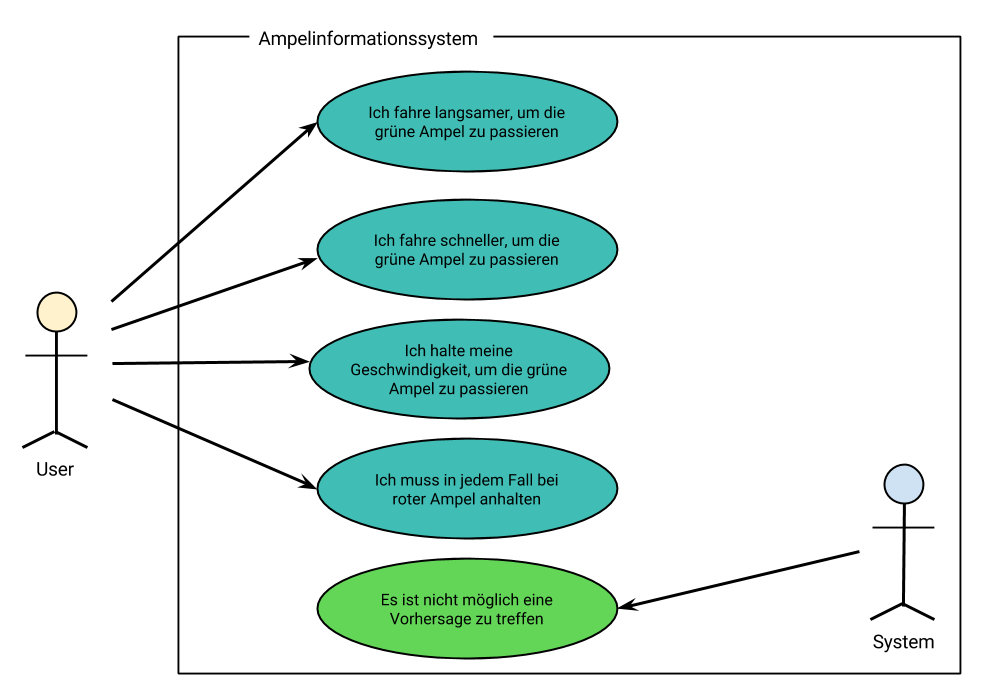
\includegraphics[width=0.8\textwidth]{uc} 
    \caption{Use-Case-Diagramm}
      \rule{35em}{0.5pt}
    \label{fig:uc}
\end{figure}
\section{Klassenarchitektur}
Die zu erstellende Anwendung erhält den Namen AIS, was für Ampel-Informationssystem steht und der vorläufige Name der Anwendung ist und besteht aus den nachfolgend beschriebenen Klassen. \\\\
Die \texttt{MainActivity} ist die Hauptklasse der Android-Applikation. Sie definiert die grafische Oberfläche der Anwendung und stellt die notwendigen Methoden bereit. \\
Der \texttt{\gls{JSON}Parser} liest die erstellte \gls{JSON}-Datei ein und wandelt deren Inhalt ein ein Array um. Dieses Beinhaltet Ampelobjekte mit deren Namen, Position und der Information darüber, ob sie verkehrsabhängig sind oder nicht. Sind sie es nicht, wird außerdem zu jeder Ampel ein Array, bestehend aus den Sigalschaltplanobjekten gespeichert. Diese enthalten benötigten alle Informationen über den Geltungszeitraum und der Grünphasen.\\ 
\texttt{GPSTracker} implementiert die Schnittstelle \texttt{LocationListener} und kann so kontinuierlich die Position des Endgeräts verfolgen. Mit der eigenen Position und der aller Ampeln aus dem vom \texttt{JSONParser} erstellten Array ermittelt er außerdem die nächste Ampel. Ist diese identifiziert, wird über den \texttt{OnSetListener} die Klasse \texttt{SpeedHandler} aktiviert, welche anhand der Daten aus dem Signalschaltplanobjekt den Countdown der Rotanzeige und die optimale Geschwindigkeit berechnet und die Anzeige entsprechend aktualisiert. \\
Das nachfolgende Klassendiagramm gibt eine Übersicht über die oben beschriebenen Klassen.
\begin{figure}[H]  
    \centering  
    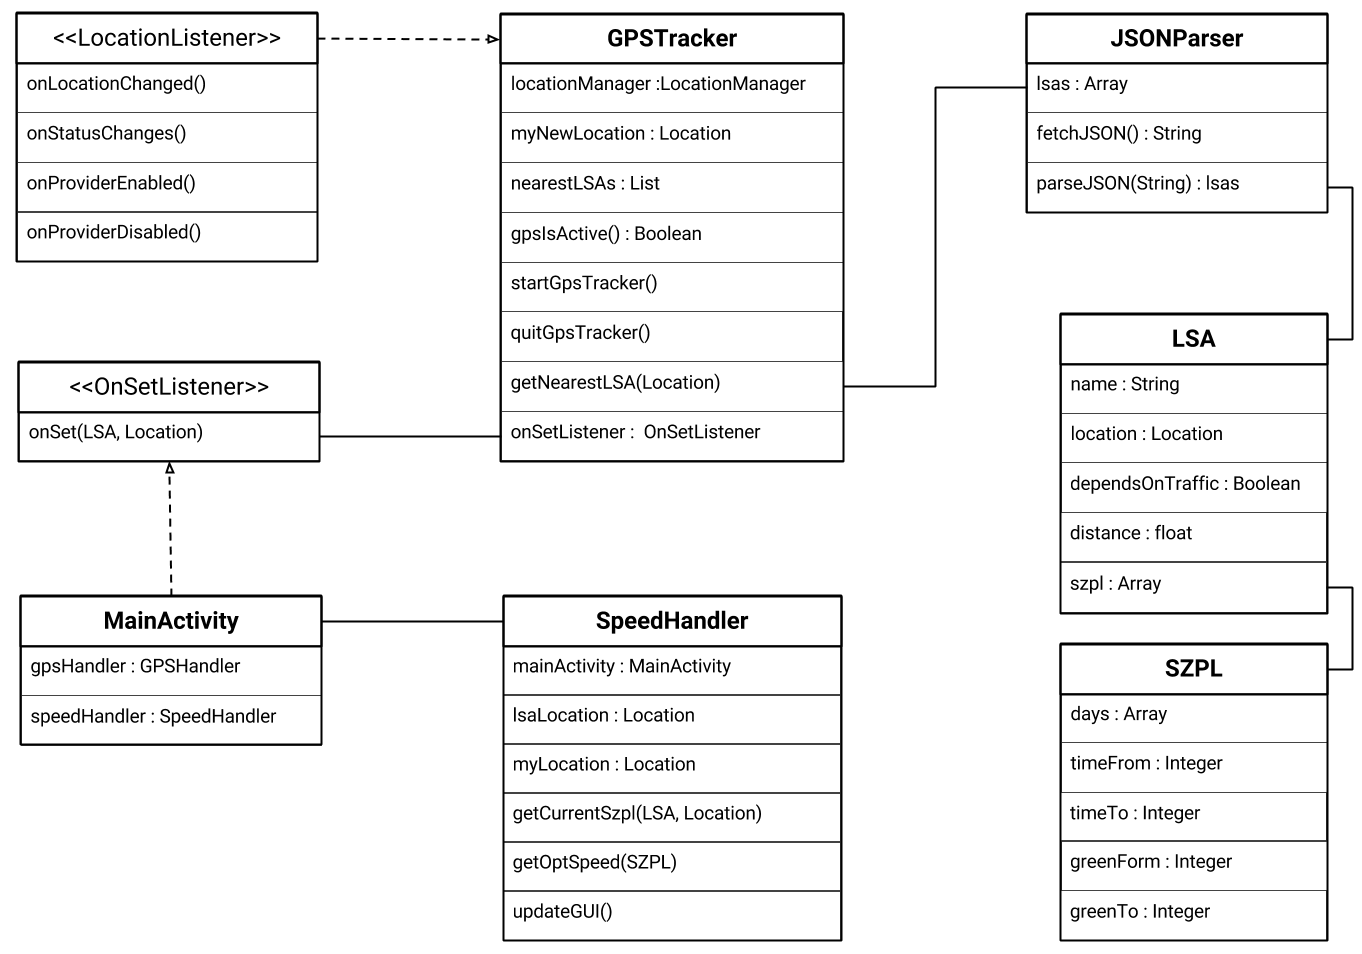
\includegraphics[width=\textwidth]{uml} 
    \rule{35em}{0.5pt}
    \caption{Klassendiagramm}
    \label{fig:uml}
\end{figure}
% ### Design ###
%\clearpage
\section{Die graphische Oberfläche}
Aus den Anforderungen an die graphische Oberfläche in Kapitel \ref{chap:anforderungen} entsteht das Design. Durch die überschaubare Anzahl an Funktionalitäten kann der Aufbau einfach gehalten werden. Aus den Empfehlungsanzeigen, welche den Systemzuständen entsprechen sind vier Ansichten abzuleiten. Die folgende Abbildung zeigt den Entwurf der Benutzeroberfläche.
Abbildung \ref{fig:stop} zeigt die grapfische Umsetzung des Zustands \textit{a}, in dem die Ampelschaltung keine Weiterfahrt ermöglicht. Es wird ein großer roter Kreis mit einem schwarzen Kreuz verwendet. Rot ist eine Signalfarbe und steht auch bei Ampeln für "'Halt"' oder "'Stop"'. Auch das Kreuz wird häufig als \textit{verweigerndes} Symbol eingesetzt und ist somit intuitiv als solches erkennbar.\\
Abbildung \ref{fig:yeah} setzt die Visualisierung des Zustands \textit{b} um, bei dem man mit der aktuellen Geschwindigkeit in der Grünen Welle fährt, um. Hier wird ist ein großer grüner Kreis verwendet, in der Mitte steht "'ok"'. Durch die nicht alleinige Benutzung der Ampelfarben Rot und Grün ist die Ansicht auch für Menschen mit einer Rot-Grün-Sehschwäche eindeutig interpretierbar.
\begin{figure}[H]
        \centering
           \begin{subfigure}[t]{0.18\textwidth}
                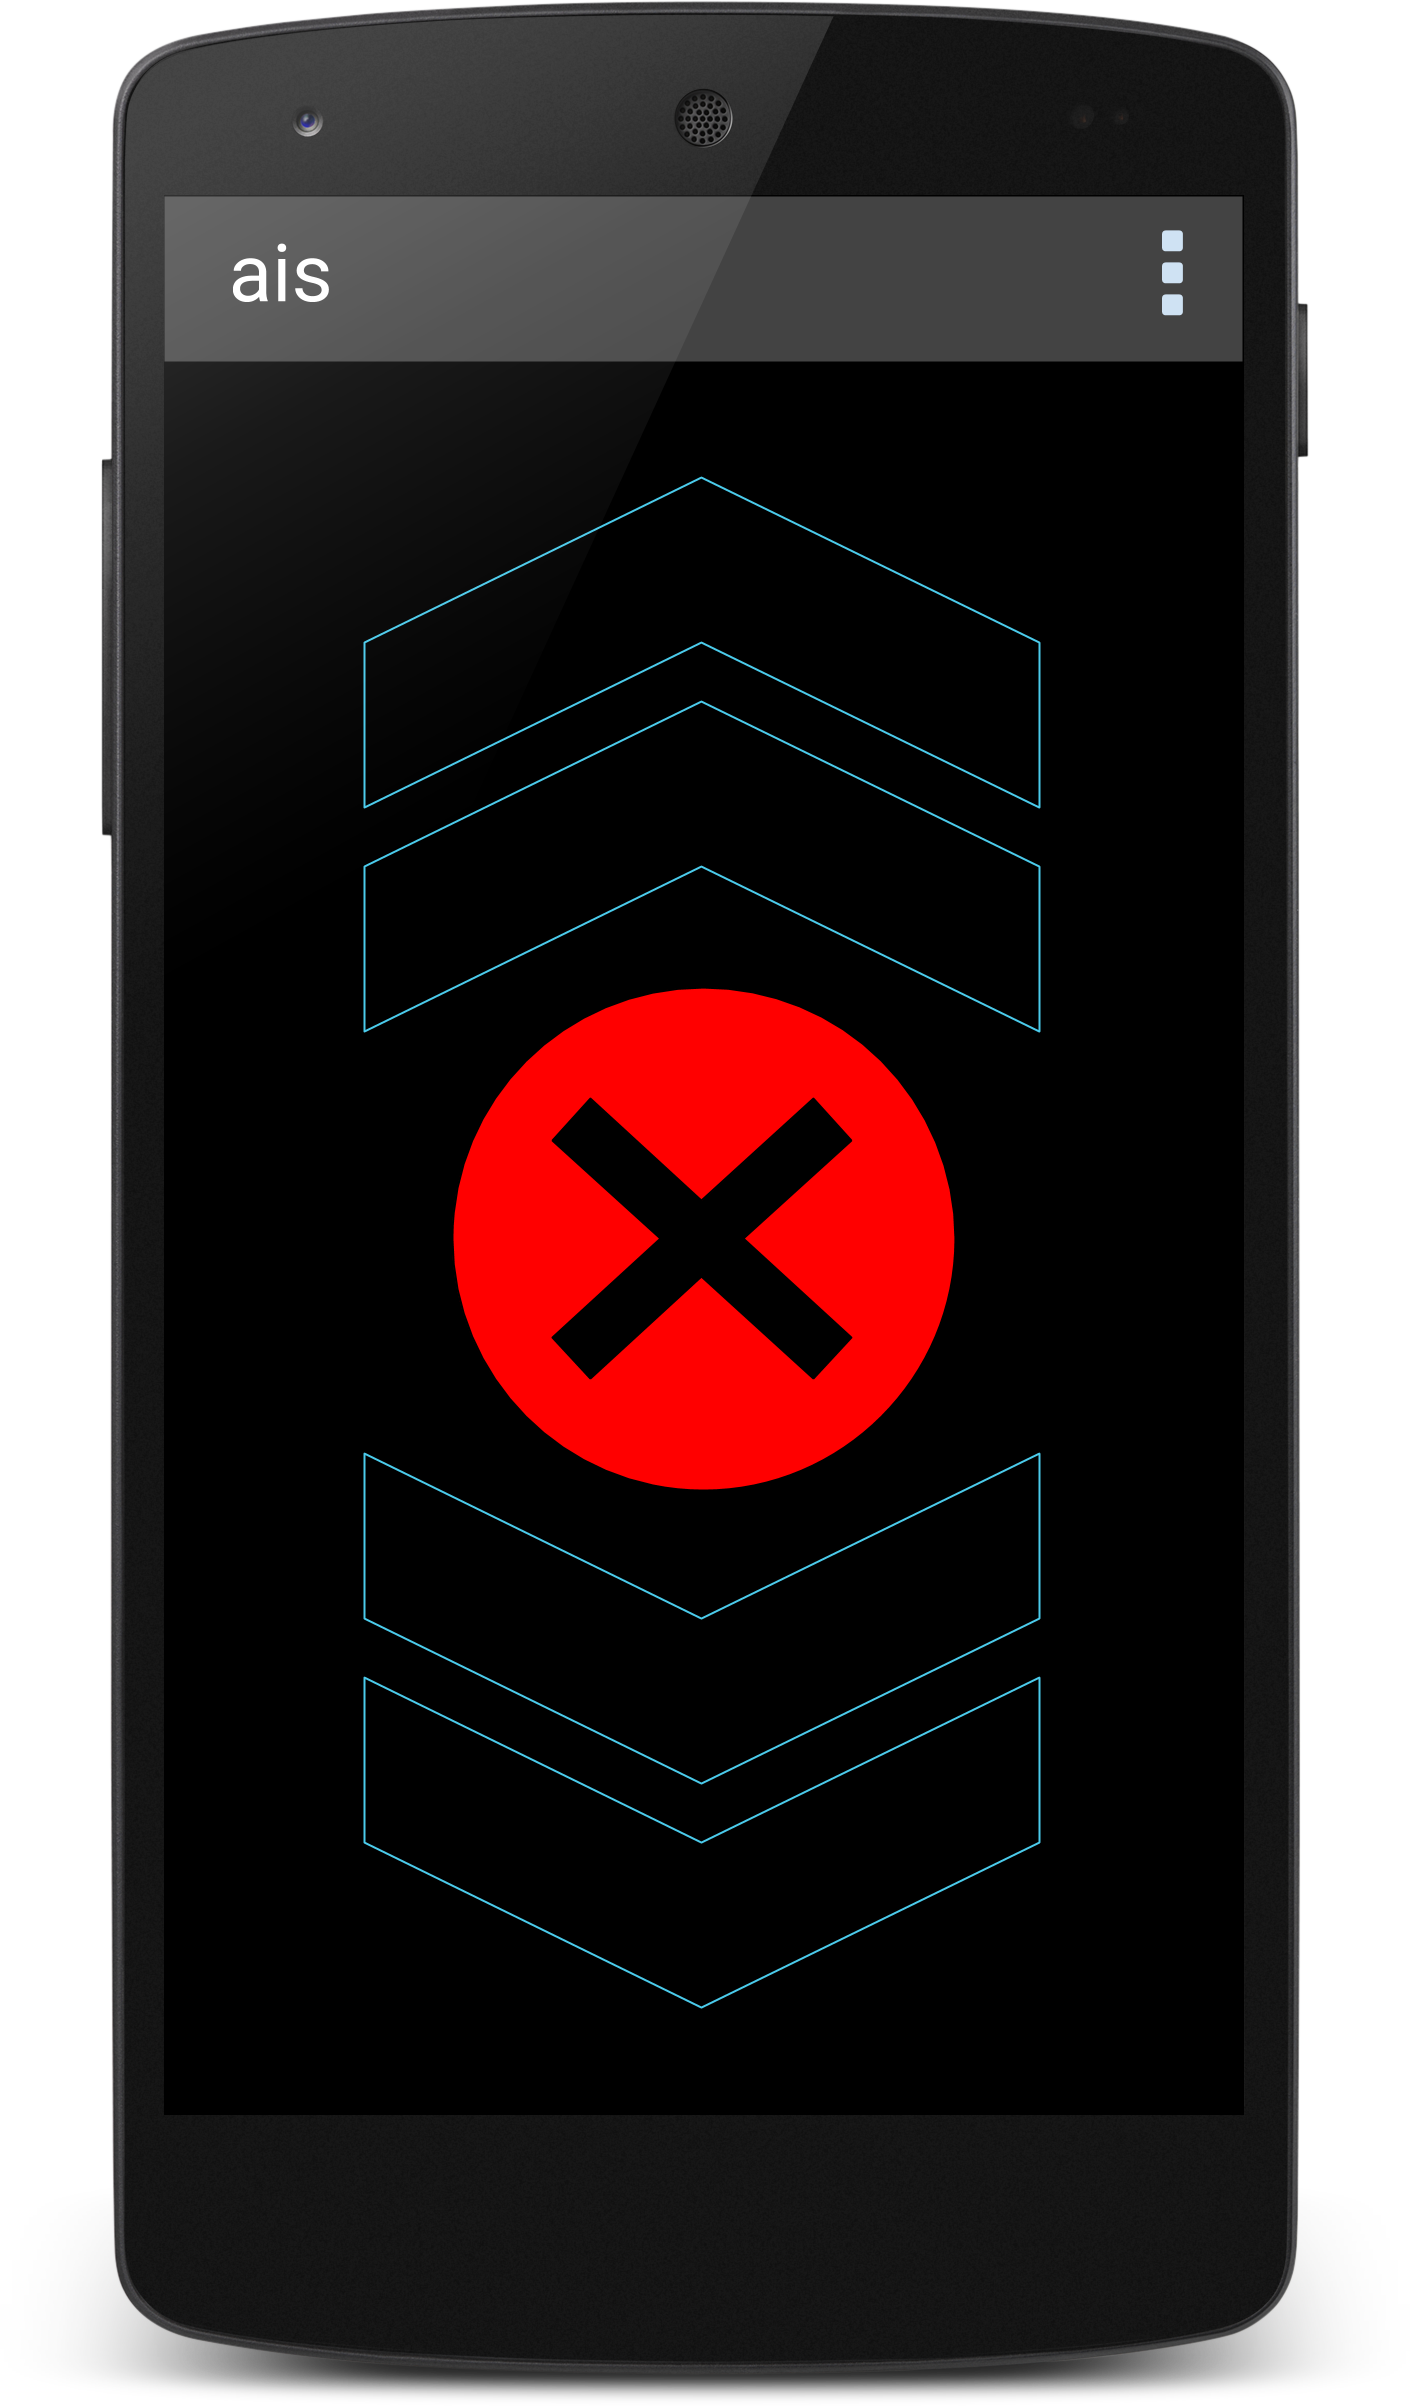
\includegraphics[width=\textwidth]{stop}
                \caption[Systemzustand a]{Anhalten an roter Ampel in jedem Fall erforderlich}
                \label{fig:stop}
        \end{subfigure}
           ~ 
              \begin{subfigure}[t]{0.18\textwidth}
                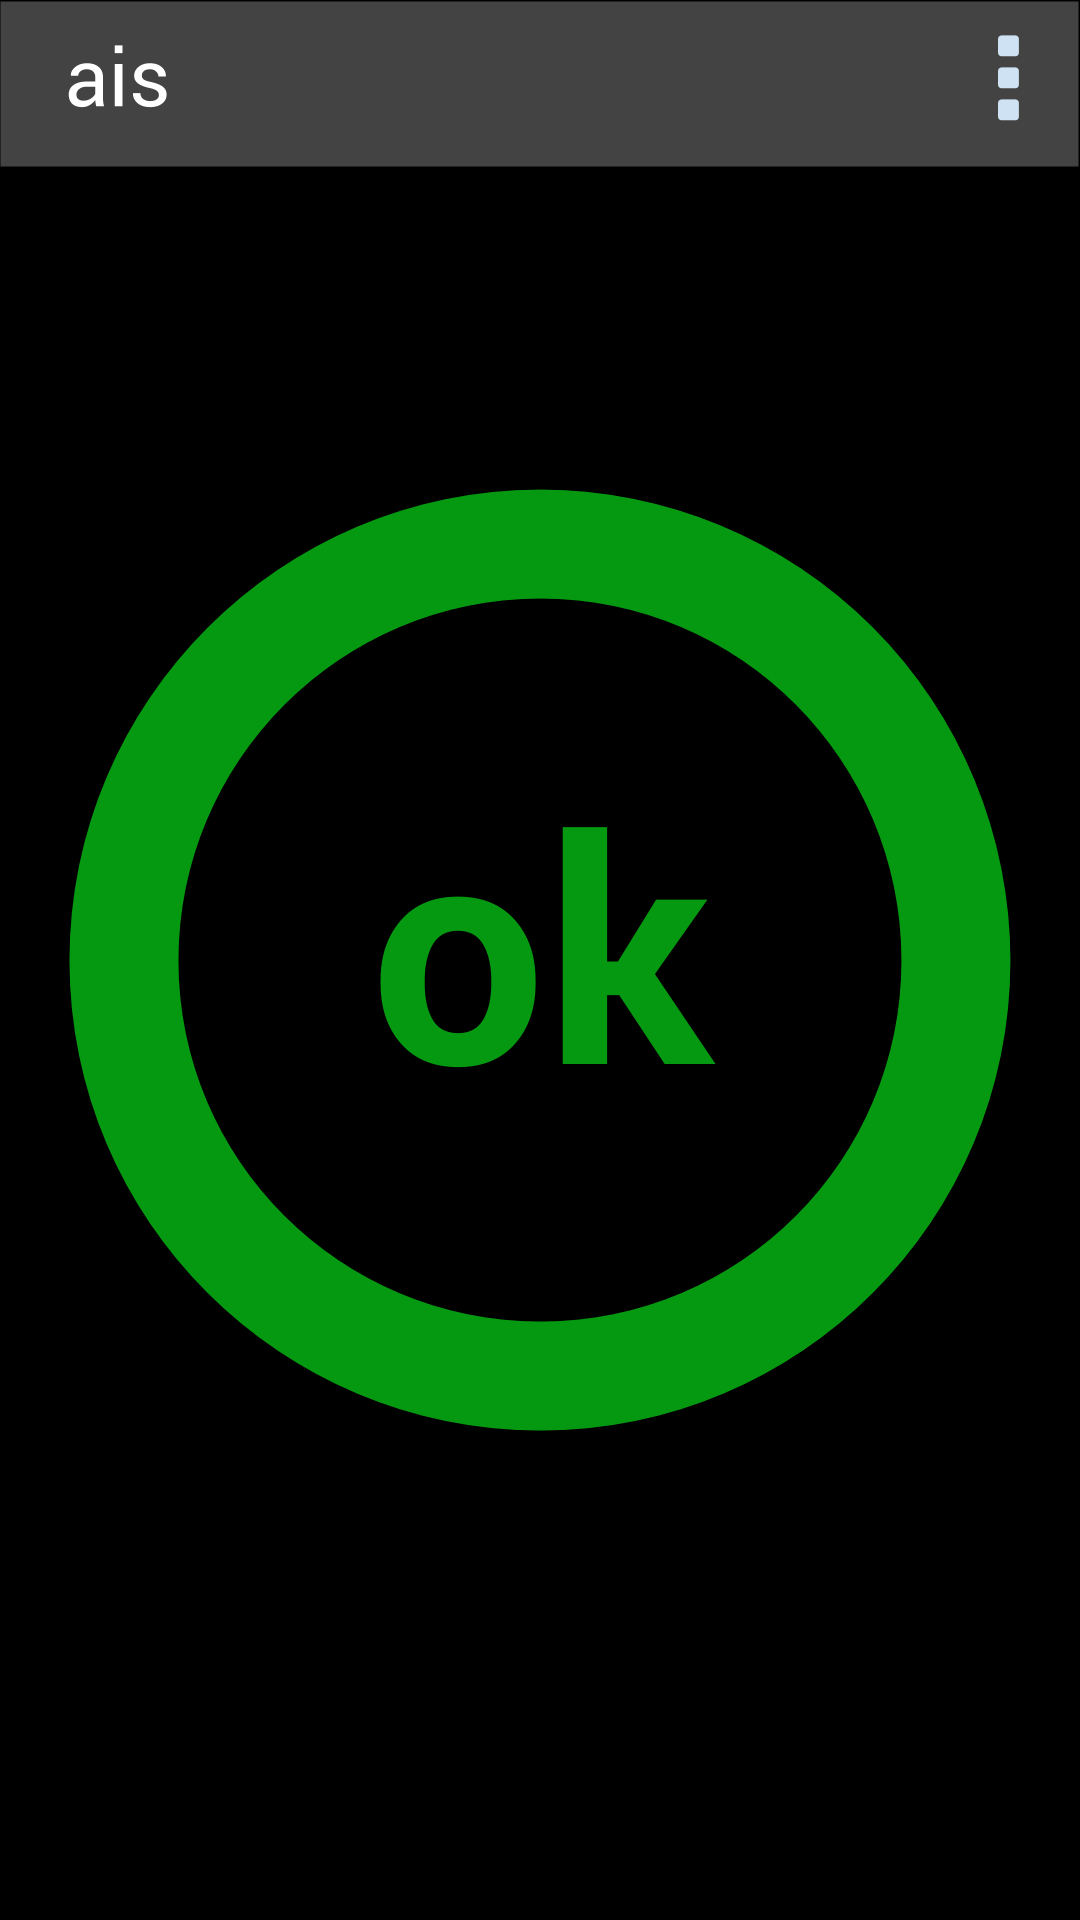
\includegraphics[width=\textwidth]{yeah}
                \caption[Systemzustand b]{Kein Aktionsbedarf}
                \label{fig:yeah}
        \end{subfigure}
           ~
        \begin{subfigure}[t]{0.18\textwidth}
                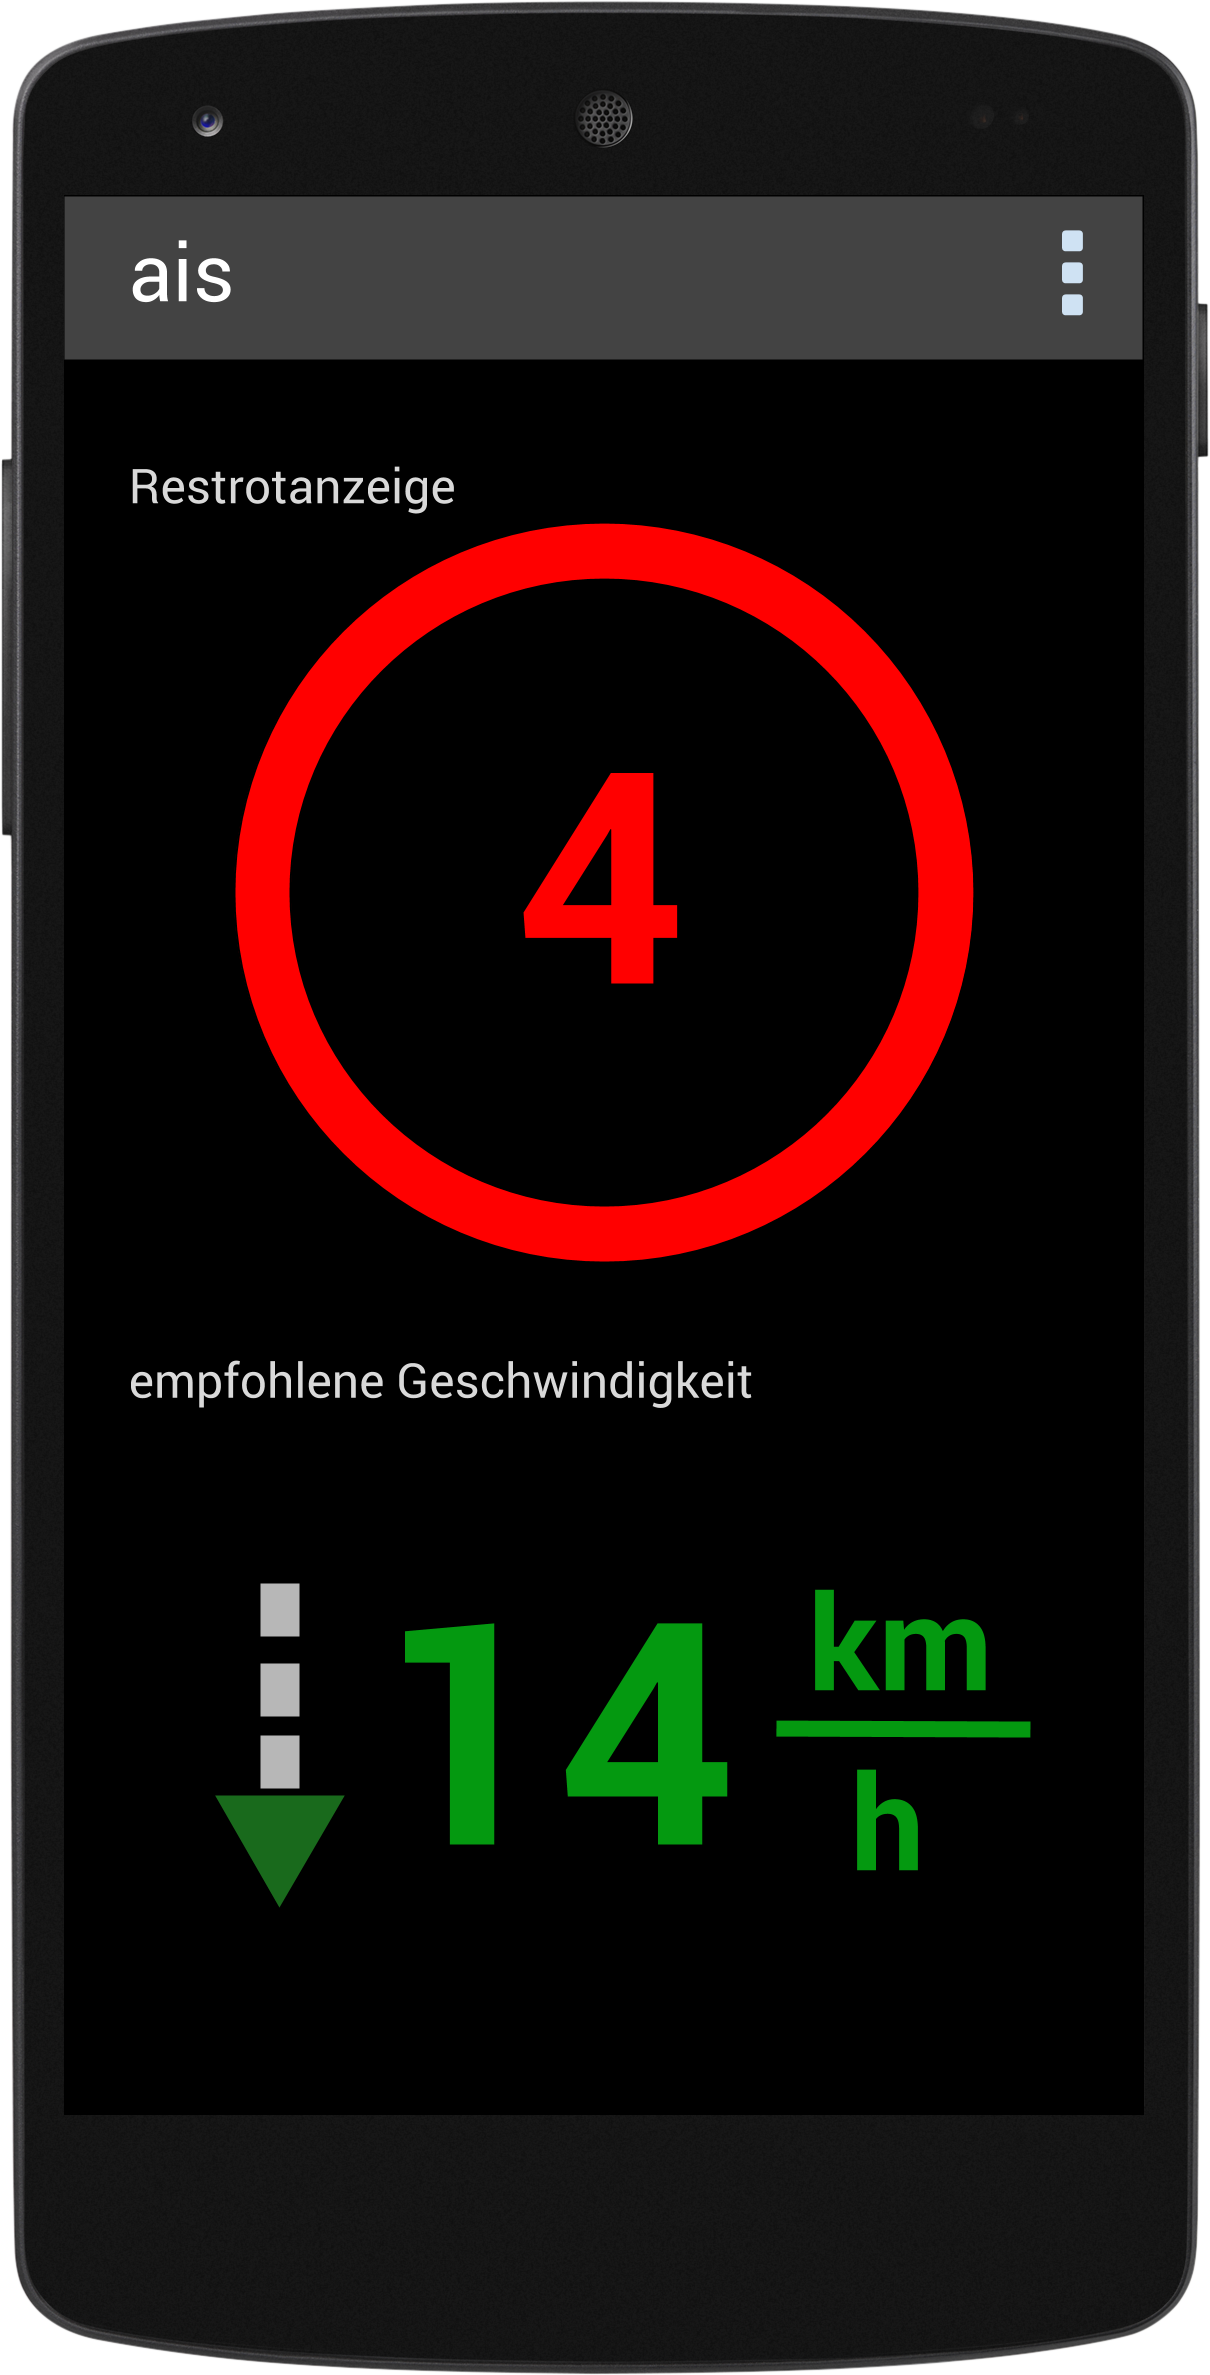
\includegraphics[width=\textwidth]{langsamer}
                \caption[Systemzustand c]{Weiterfahrt durch Verlangsamung  möglich}
                \label{fig:langsamer}
        \end{subfigure}
        ~
        \begin{subfigure}[t]{0.18\textwidth}
                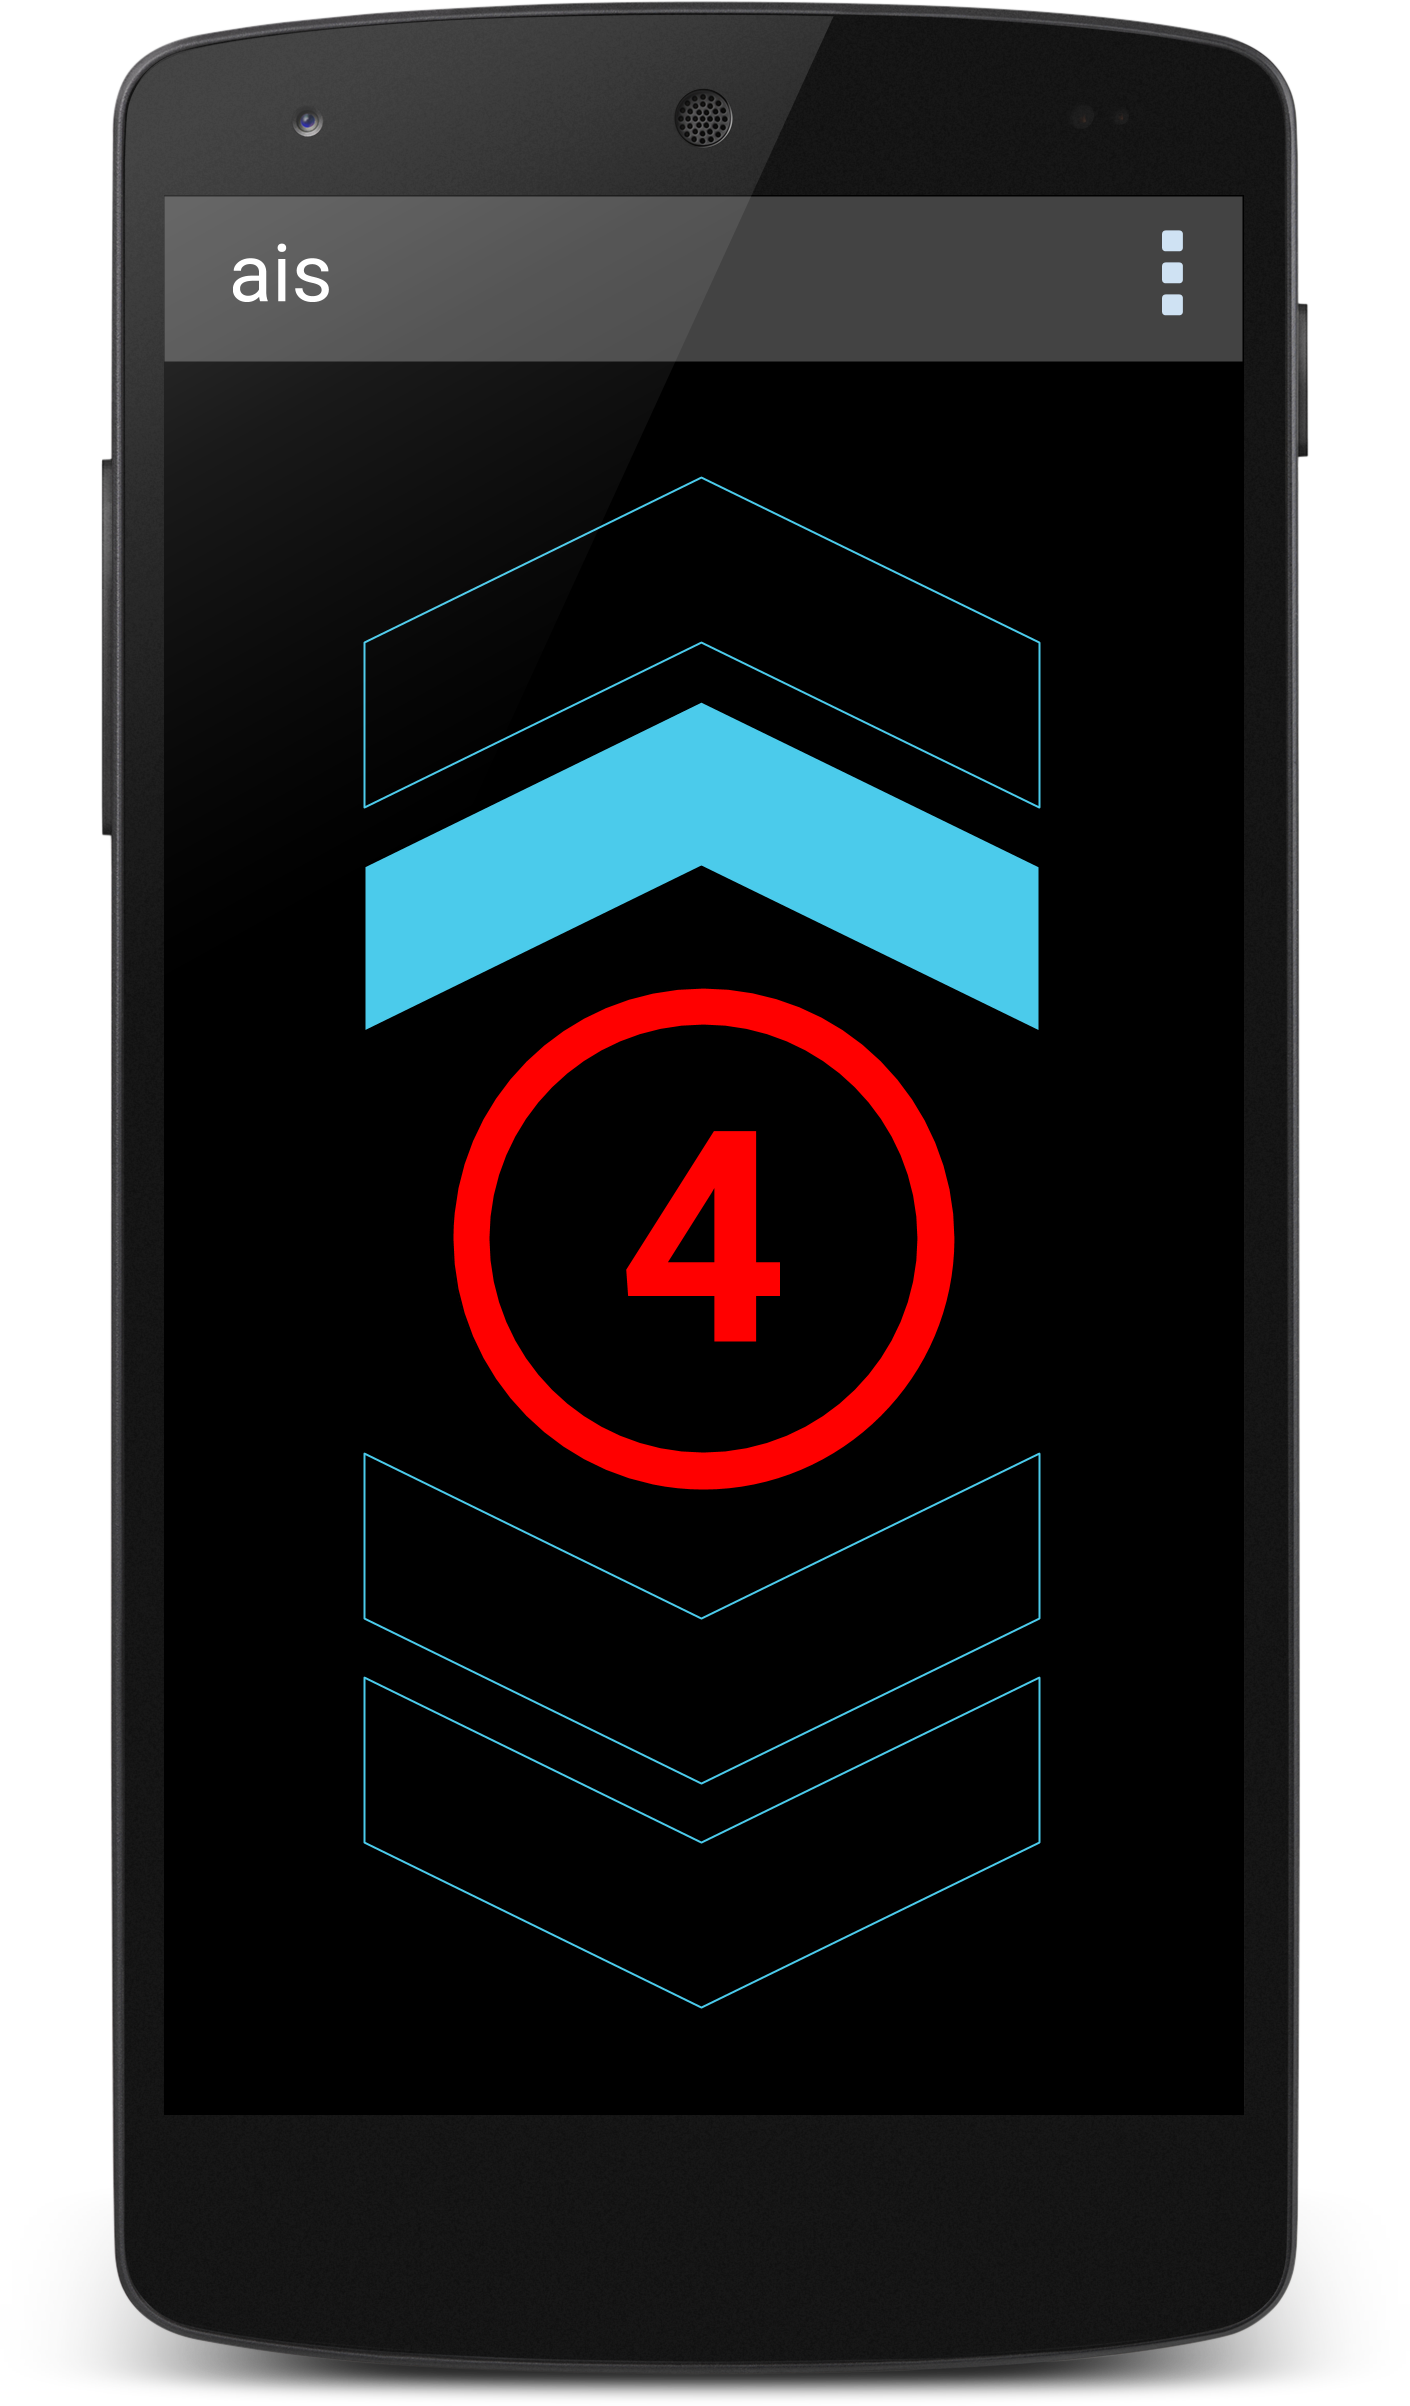
\includegraphics[width=\textwidth]{schneller}
                \caption[Systemzustand d]{Weiterfahrt durch Beschleunigung möglich}
                \label{fig:schneller}
        \end{subfigure} 
        ~ 
        \begin{subfigure}[t]{0.18\textwidth}
        	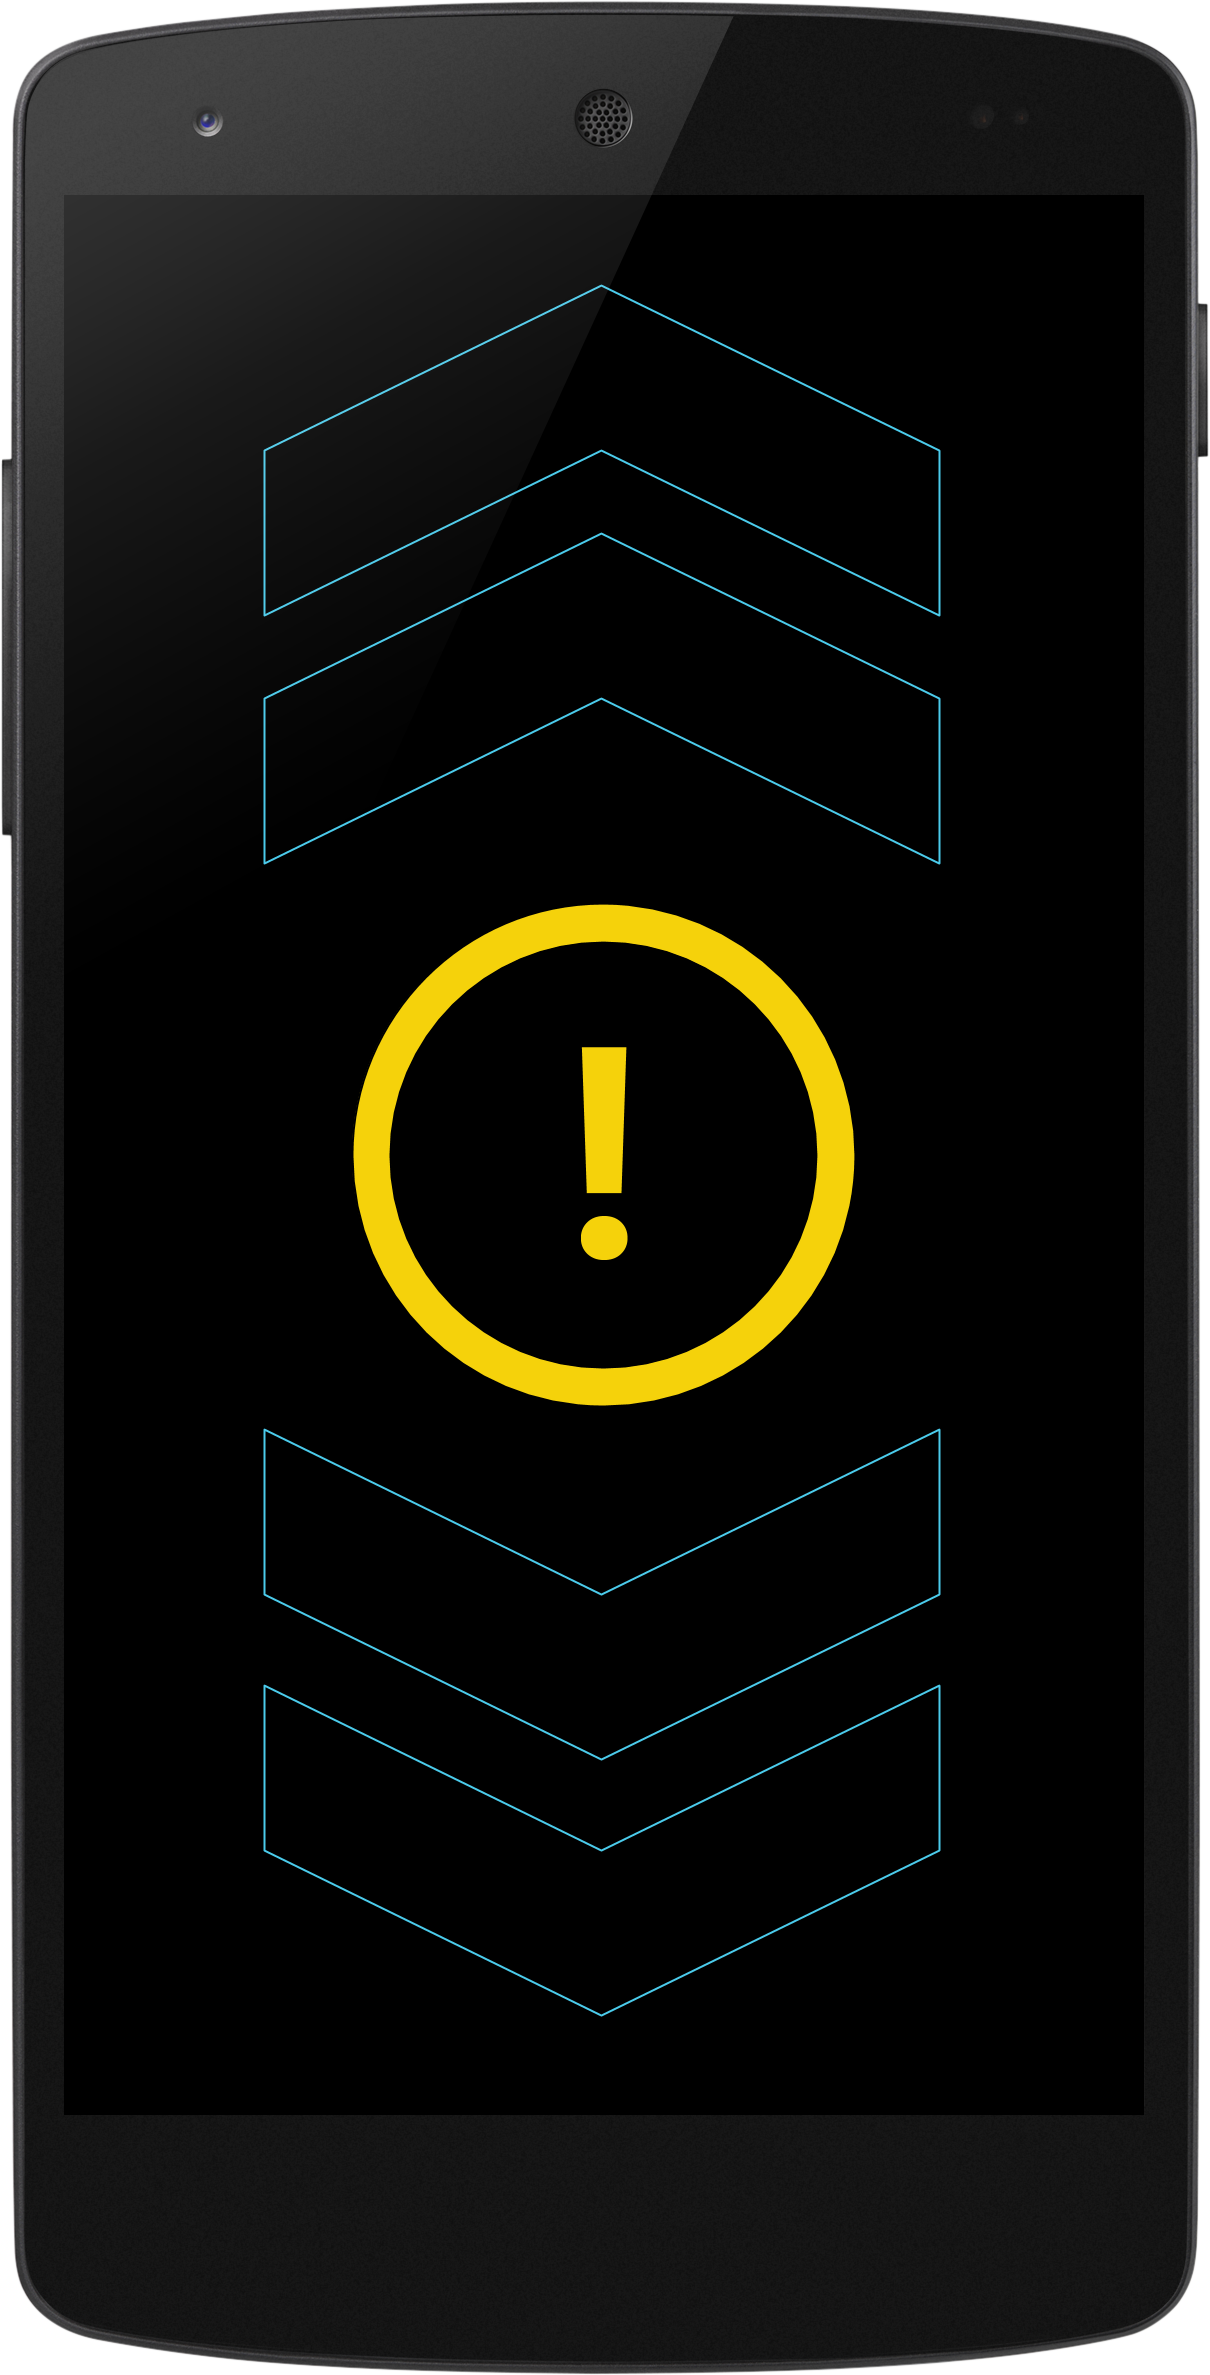
\includegraphics[width=\textwidth]{mep}
        	\caption[Systemzustand e]{Keine Vorhersage möglich}
            \label{fig:meh}
        \end{subfigure} 
        \rule{35em}{0.5pt}   
        \caption[Systemzustände im Ampelbereich]{Entwurf des Designs anhand der Systemzustände}
        \label{fig:mockup}
\end{figure}
Die Abbildungen \ref{fig:langsamer} und \ref{fig:schneller} für die Zustände \textit{c} und \textit{d} sind in der Anordnung der Elemente identisch. Mittig im Bild ist eine eingekreiste rote Zahl die den Countdown der Restrotanzeige darstellt. Sie wird also mit jeder Sekunde aktualisiert. Ober- und unterhalb des Countdowns befinden sich jeweils zwei hellblaue Pfeile. Je nach Differenz der aktuellen zur berechneten Geschwindigkeit sind ein oder zwei Pfeile ausgefüllt. Wird also empfohlen viel schneller zu fahren, sind die oberen Pfeile aktiv, bei der Aufforderung etwas das Tempo zu drosseln der untere. Es sind immer alle Pfeile zu sehen. Durch die Anzeige "'ein von zwei"' ist die Bedeutung der Geschwindigkeitsstufen klarer. Als Farbe für die Pfeile wurde Hellblau gewählt. Sie unterscheidet sich sowohl farblich als auch in der Helligkeitsstufe zu den anderen Farben und steht im hohen Kontrast zu dem Hintergrund. Auf schwarzem Hintergrund wirken die Farben intensiver und sind so auch aus dem Augenwinkel leichter zu erkennen und unterscheiden. Die in Abbildung \ref{fig:meh} gezeigte Darstellung erscheint, wenn keine Vorhersage möglich ist weil die Ampel verkehrsabhängig und die Vorhersage dadurch zu ungenau wird. Als Farbe wurde die dritte Ampelfarbe Gelb gewählt, was weder Rot für Anhalten, noch grün für Weiterfahren ist und so signalisiert, die Anwendung kann keine Empfehlung aussprechen. Das mittig platzierte Fragezeichen unterstützt die Aussage.\\
Die aktuelle Geschwindigkeit wird bewusst nicht angezeigt. Auch nicht die Progressionsgeschwindigkeit. Die Differenz ist beim Fahrrad nicht so hoch wie bspw. im Auto. Bei einer Varianz von wenigen km/h genügt die Anzeigevariante "'schneller"' und "'noch schneller"'.
% TESTFÄLLE
\section{Testfälle}
Folgende Testfälle werden während der Entwicklung stetig durchgeführt. Das erfolgreiche Bestehen dieser Tests ist eine notwendige Qualitätseigenschaft der zu entwickelnden Applikation.
\begin{description}[leftmargin=0.7cm,style=nextline]
\item[Sicherheitshinweis:] 
Die Anwendung muss nach jeder Installation auf den Vorrang der Verkehrssicherheit hinweisen und auf die Bestätigung des Nutzers oder der Nutzerin warten.\\
\item[Anwendung starten:] 
Die Anwendung muss sich zu jedem Zeitpunkt starten lassen. \\
\item[Anwendung beenden:] 
Die Anwendung muss sich zu jedem Zeitpunkt beenden lassen. \\
\item[Einlesen der Datei:] 
Die am nächsten gelegene Ampel und deren Rot- oder Grünphase kann nur ermittelt werden, wenn die Daten richtig eingelesen werden. Auch kann der Countdown der Restrotanzeige nur mit den Daten des Schaltplans angezeigt werden.\\
\item[Ermittlung der Position:] 
Die Empfehlung der Geschwindigkeit kann nur dann korrekt angezeigt werden, wenn die Position des Geräts ermittelt wurde. Weiter wird der eigene Standort neben dem der Ampel für die Berechnung der am nächsten gelegenen \gls{LSA} benötigt.\\
\end{description}
\section{Entwicklungsumgebung}
Für die Erstellung der Smartphone-Applikation wurde folgende Soft- und Hardware verwendet:
\subsubsection{Software}
\begin{itemize}
	\item Android Studio\footnote{ Download unter \url{http://developer.android.com/sdk/index.html}} Version 1.1. Enthält Android Studio IDE, Android \gls{SDK}-Tools, Android 5.0 Plattform, Android 5.0 Emulator System Image mit Google \glspl{API}
	\item git, Version 1.7.10.4
\end{itemize}
\subsubsection{Hardware}
\begin{itemize}
	\item Lenovo Thinkpad W520 (Intel\textsuperscript{\textregistered} Core\texttrademark   i7-2630QM, 2,00GHz, 4GB RAM) als ersten Entwicklungsrechner (Betriebssystem: Debian\footnote{ Download unter \url{https://www.debian.org/index.de.html}} 7.8, 64-bit-Version)
	\item Lenovo Thinkpad X200 (Intel\textsuperscript{\textregistered} Core\texttrademark   i7-2630QM, 2,00GHz, 8GB RAM) als zweiten Entwicklungsrechner (Betriebssystem: Debian 7.8, 64-bit-Version)
	\item Android Testgeräte: Samsung Galaxy Note 2, LG Nexus 5
\end{itemize}

         
\chapter{\label{chap:implementierung}Der Prototyp}
In diesem Kaptitel wird die nach dem in Kapitel \ref{chap:entwurf} präsentierten Lösungswegs die detaillierte Beschreibung der technischen Realisierung der Anwendung vorgestellt.\\
Nach der Erklärung der Konfigurationsdateien wird auf die Umsetzung der Szenarien eingegangen. Im Zuge dessen werden die implementierten Algorithmen vorgestellt, wobei sich der erste mit dem Auffinden der nächsten relevanten Ampel befasst und der zweite die empfohlene Geschwindigkeit berechnet.
%
% MANIFEST
%
\section{Die Manifest- und build.gradle-Datei}
Das Android-Manifest dient der Festlegung wichtiger Eigenschaften der Anwendung und gehört zu jedem Android-Projekt. Die \gls{XML}-Datei (\texttt{AndroidManifest.xml}) ist im Hauptverzeichnis des Projekts zu finden und im Listing \ref{lst:manifest} abgebildet. In der zweiten Zeile wird hier der Paketname des Programms festgelegt. 
\begin{center}
\rule{35em}{0.5pt} \lstinputlisting[language=XML, firstline=2, lastline=21, caption={AndroidManifest.xml}, label=lst:manifest]{code/manifest.xml}
 \rule{35em}{0.5pt}
\end{center}
Im \texttt{application}-Tag werden Variablen gesetzt, die das in dargestellte Icon und den Namen der Anwendung definieren. Darüber hinaus wird hier die \gls{Activity} der Applikation definiert. Zuerst wird der Name der \gls{Activity} gesetzt. Die Variable \texttt{screenOrientation} legt das Format der Anzeige fest und verhindert ein automatisches Drehen des Bildschirms. \\
Im \texttt{intent-filter}-Tag dass diese Activity beim Start der App ausgeführt wird. Hätte die Anwendung über mehrere \glspl{Activity} implementiert, würden die anderen ebenfalls hier aufgeführt werden.
Unterhalb des \texttt{application}-Tags, in Zeile 17, werden nun die Berechtigung des \gls{GPS}-Zugriffs der Applikation, um Standortdaten, also die jeweiligen geographischen Kordinaten des Endgeräts zu beziehen gesetzt.\\\\
Android Studio-Projekte enthalten eine Top-Level-Build-Datei und eine Build-Datei für jedes Modul. Die Build-Dateien heißen \texttt{build.gradle} und sind einfache Textdateien, die die Groovy\footnote{ Programmier- und Skriptsprache}-Syntax verwendend. Hier lässt sich der Build mit den Elementen, welche vom Android Plugin Gradle\footnote{ Gradle ist ein auf Java basirerndes Build-Management-Automatisierungs-Tool.} unterstütz werden, konfigurieren. \cite{android_build} \\ 
Listing \ref{lst:gradle} zeigt einen Ausschnitt aus der Build-Datei für die Anwendung. \\
Die Eigenschaft \texttt{compileSdkVersion} beschreibt mit welcher Android \gls{SDK} Version kompiliert werden soll und \texttt{buildToolsVersion} gibt an, welche Version des Build-Tools verwendet wird.
\begin{center}
\rule{35em}{0.5pt} \lstinputlisting[language=JSON, firstline=6, lastline=14,  caption={Auszug aus der build.gradle-Datei}, label=lst:gradle]{code/build.gradle} \rule{35em}{0.5pt}
\end{center}
Es folgt das \texttt{defaultConfig} Element, das die Kerneinstellungen und fügt diese dynamisch aus dem Build-System in die  Manifestdatei ein. Hier wird unter anderem festgelegt, für welche Android Versionen die Anwendung geschrieben wurde (\texttt{targetSdkVersion}) und das minimale \gls{API}-Level\footnote{ Eine Übersicht über die \gls{API}-Level und der dazugehörigen Android-Version findet sich unter \url{http://developer.android.com/guide/topics/manifest/uses-sdk-element.html} -- Zugriff: 03.03.2015} der Anwendung (\texttt{minSdkVersion}).\\ 
Letzteres ist auf "'10"' gesetzt und zeigt, dass die Anwendung auf Mobilgeräten auf denen mindestens die Android-Version 2.3.3 installiert sein muss. 
Die Android-Version wurde auf 2.3.3 festgelegt, da das die Mindestanforderung für das editieren der \texttt{SharedPreferences}, welche für das einmalige Anzeigen des Warndialogs benötigt werden, ist. Damit werden trotzdem noch 99,6\% der Geräte, die auf den Google-Play-Store zugreifen können, abgedeckt. \cite{android_version} 
%
% MainActivity
%
\clearpage
\section{MainActivity-Klasse}
Die Klasse \texttt{MainActivity} ist die \gls{Activity}, die beim Start der Anwendung ausgeführt wird.  Hier werden die Anzeigeelemente initialisiert und die zentralen Funktionalitäten delegiert.\\
Die Methode \texttt{onCreate} ist die erste Methode im \gls{Activity}-Lebenszyklus\footnote{ \url{http://developer.android.com/training/basics/activity-lifecycle/starting.html} -- Zugriff: 02.03.2015} und wird direkt nach dem Start der \gls{Activity} ausgeführt. Hier werden die Anzeigeelemente gesetzt und nach jeder Installation ein Dialog erstellt, der auf die oberste Priorität der Straßenverkehrsordnung hinweist.\\
Es wird eine Instanz des \texttt{JSONParser}-Objekts erstellt, welche die \gls{JSON}-Datei aus dem Ressourcenordner liest und in ein Objektarray umwandelt. Neben der \texttt{SpeedHandler}-Objektinstanz, welche für die Geschwindigkeitsempfehlung und dessen Anzeige zuständig ist, wird die des \texttt{GPSTracker} erstellt. Auf diesen ist der \texttt{OnSetListener} registriert, welcher ein Ereignis wirft sobald er die nächstgelegende Ampel gesetzt hat. Sobald dieser Fall eingetreten ist, wird der \texttt{SpeedHandler} beauftragt, den dazugehörigen Signalschaltplan zu holen, um dann anhand dieser Daten die Berechnungen durchzuführen und deren Ergebnisse anzuzeigen.   
%
% Umsetzung Szenarien
%
\section{Umsetzung Szenarien}
Wie in Kapitel \ref{chap:szenarien} beschrieben, lassen sich die sieben möglichen Szenarien auf insgesamt fünf komprimieren, da die Szenarien R2 und G2, genauso wie die Szenarien R3 und G3 dasselbe Ergebnis haben. Die zusammengefassten fünf Szenarien eignen sich für eine prototypische Umsetzung, welche im Folgenden beschrieben wird.
%
% Einlesen der Ampeldaten
%
\subsection{Einlesen der Ampeldaten}
Neben der Geräteposition bilden die Ampelposition und deren Signalschaltpläne die Grundlage der Anwendung. Hierbei ist das korrekte Einlesen und Auswerten der Daten obligatorisch. Die Aufgabe des \texttt{JSONParsers} ist es also, die manuell erstellte \gls{JSON}-Datei, welche die Ampeldaten beinhaltet, richtig zu konvertieren. Die Klasse \texttt{JSONParser} liest also die Datei ein und wandelt dann die enthaltenen \gls{JSON}-Ampelobjekte in Java-Ampelobjekte um.\\ 
Hierfür wird das \gls{JSON}-Array durchlaufen und für jedes enthaltende Objekt ein Ampelobjekt erzeugt. Aus den Werten \texttt{lat} und \texttt{lon}, stehend für latitude und longitude, wird ein \texttt{Location}-Objekt erzeugt, das als Attribut gesetzt wird. Der boolsche Wert \texttt{dependsOnTraffic} ist auf \texttt{true} gesetzt, sobald die \gls{LSA} verkehrsabhängig ist. Ist dies der Fall, ist eine Vorhersage der Ampel aufgrund beeinflussender Parameter nicht möglich und es wird ein Objekt mit den beiden genannten Attributen und dem bezeichnenden Namensattribut erzeugt. Andernfalls werden die zu der Ampel hinzugehörigen Schaltpläne durchlaufen und für jeden ein selbiges Objekt erzeugt, welche in einem Array gespeichert dem Ampelobjekt als weiteres Attribut übergeben wird. Es ist zu beachten, dass jeder Signalschaltplan über ein Array mit Tagen verfügt. Denn ein Schaltplan kann an mehreren Tagen gültig sein. Die Tage sind als Strings gespeichert und werden für die weitere Verwendung in Integer umgewandelt, wobei die Woche am Sonntag beginnt. Der Sonntag wird also als \texttt{1} gespeichert, der Montag als \texttt{2} und so weiter. 
%
% nächste Ampel
%
\subsection{Ermittlung der nächsten Ampel}
Zur Ermittlung der nächsten Ampel ist zunächst die eigene Position vonnöten. Dazu stellt der in dem \texttt{android.location}-Paket enthaltene \texttt{LocationManager} die entsprechenden Schnittstellen bereit. Für den Empfang der \gls{GPS}-Daten implementiert die Klasse \texttt{GpsTracker} das \texttt{LocationListener} Interface und registriert sich beim \texttt{LocationManager} für \gls{GPS}-Updates.
Letzteres ist im Listing \ref{lst:gps1} abgebildet. Die Methode erwartet neben dem Providertyp und dem zu benachrichtigenden Listener (\texttt{this}) zwei weitere Parameter. Der erste zeigt an nach wie vielen Millisekunden ein Update gesendet werden soll, der zweite dass ein Update nur gesendet werden soll, wenn sich die Position um die angegebene Distanz verändert hat.
\begin{center}
\rule{35em}{0.5pt}
\lstinputlisting[language=Java, firstline=1, lastline=3, caption={Registrierung für GPS-Updates in GpsTracker.java}, label=lst:gps1]{code/gpstracker.java}
\rule{35em}{0.5pt}
\end{center}
Zusammen mit dem \texttt{LocationListener} wird unter anderem die Methode \texttt{onLocationChanged}, welche aufgerufen wird sobald neue Positionsdaten vorhanden sind implementiert. Das hier gespeicherte \texttt{Location}-Objekt liefert neben dem Längen- und Breitengrad auch die Genauigkeit des \gls{GPS}-Signals in Metern und Geschwindigkeit in Metern pro Sekunde. Sofern die Genauigkeit nicht zu gering ist, wird mit ihm wird die Methode \texttt{getNearestLSA} aufgerufen, welche die nächste Ampel bestimmt.\\
Die Methode \texttt{getNearestLSA} ermittelt zunächst alle Ampeln im festgelegten Radius und speichert diese zusammen mit der Distanz zum Gerät in einer temporären Liste. Dann werden diese wieder durchlaufen und die Distanzen verglichen. Die Ampel, zu der sich die Entfernung zum Gerät verringert und die kleinste Distanz zum Gerät hat, ist die Gesuchte. Ist die nächste Ampel ermittelt, kann der \texttt{OnSetListener} der \texttt{MainActivity} diese zusammen mit der Geräteposition übergeben. \\\\
Vergrößert sich die Distanz zu der \gls{LSA} wieder befindet sie sich außerhalb des durchsuchten Radius bedeutet das, dass der Fahrer oder die Fahrerin sich von der Ampel oder der Kreuzung entfernt. Also werden diese dann zusammen mit den anderen gespeicherten Ampeln gelöscht. 
\clearpage
\begin{center}
%\rule{35em}{0.5pt}
\lstinputlisting[language=Java, firstline=12, lastline=64, caption={Ermittlung der nächsten LSA in GpsTracker.java}, label=lst:gps]{code/gpstracker.java}
%\rule{35em}{0.5pt}
\end{center}
%
% v = s/t
%
\subsection{Berechnung der Geschwindigkeitsempfehlung}
An dieser Stelle wird die Berechnung der Geschwindigkeitsempfehlung erklärt. Sobald alle benötigten Daten bestehend aus aktueller, eigener Position, Entfernung zur nächsten Ampel und deren Signalschaltplan wird die benötigte Geschwindigkeit errechnet, die Ampel bei Grün zu erreichen. Diese Geschwindigkeit wird mit er Formel: 
\[ v = \frac{s}{t_{2} - t_{1}} \]
berechnet, wobei $t_1$ die aktuelle Sekunde, $t_2$ der Zeitpunkt zu dem die Ampel auf Rot schaltet und $s$ die Entfernung zur Ampel ist. \\
Für FahrradfahrerInnen ist die Beschleunigung ebenfalls von nicht geringer Bedeutung, weil sie begrenzt ist. Die Formel für die Beschleunigung lautet:
\[ a = \frac{v}{(t_{2} - t_{1})^{2}} \] 
Die Variable $v$ ist hier die errechnete Empfehlungsgeschwindigkeit.\\\\
Anhand der errechneten Geschwindigkeit, Beschleunigung und Geschwindigkeit des Geräts wird das \gls{GUI} aktualisiert. Hier wird berücksichtigt, ob die errechnete Geschwindigkeit, sowie die Beschleunigung innerhalb festgelegter Parameter liegen. Da bei einer Handlungsaufforderung zusätzlich zur Empfehlung der Countdown der Ampel dargestellt wird, geschieht dies sekündlich.\\
Jede \gls{App} hat ihren eigenen \gls{UI}-Thread und nur Objekte, die auf dem \gls{UI}-Thread ausgeführt werden haben Zugang zu anderen Objekten auf diesem Thread. Um Daten aus einem Hintergrundthread auf den \gls{UI}-Thread zu verschieben wird der \texttt{Handler} verwendet.
Also wird in der umsetztenden \texttt{SpeedHandler}-Klasse eine \texttt{Handler}- und eine \texttt{Runnable}-Instanz erzeugt. Ein \texttt{Handler} ist eine Schnittstelle für die Kommunikation zwischen Threads. Jede \texttt{Handler}-Instanz wird mit einem Thread und dessen Warteschlange verbunden. Ein \texttt{Runnable} ist ein Objekt, das etwas ausführen kann. Das \texttt{Runnable} wird nun mittels \texttt{post()} im \texttt{Handler} abgelegt, wodurch \texttt{Runnable} aus dem \texttt{Handler} im \gls{UI}-Thread ausgelesen und gestartet wird. 
%
% Installationsanleitung
%
\section{Installationsanleitung}
Um die Anwendung zu installieren muss deren .apk-Datei auf das Gerät geladen und von dort gestartet werden. Die .apk-Datei ist das als Zwischencode ausführbare Kompilat, welches dann auf dem Gerät zu Plattformcode kompiliert wird. Zum Auffinden und ausführen der Datei wird ein Dateimanager, wie zum Beispiel der kostenlose ASTRO File Manager\footnote{ Der ASTRO File Manager steht im Google Play Store unter \url{https://play.google.com/store/apps/details?id=com.metago.astro&hl=de} bereit.}  benötigt. 

\chapter{Evaluation}
Um die Funktionalität des Prototyps zu untersuchen, wurden folgende Testgeräte ausgewählt. Es handelt sich hierbei um Geräte mit unterschiedlichen Bildschirmgrößen und Android-Versionen.\\ 
\begin{table}[H]
\centering	
	\begin{tabular}{@{}>{\columncolor[HTML]{ECF4FF}}l ll@{} p{0.4\textwidth}p{0.2\textwidth}p{0.2\textwidth}} \toprule	
\multicolumn{1}{c}{\cellcolor[HTML]{ECF4FF}\textbf{Testgerät}} 
& \multicolumn{1}{c}{\cellcolor[HTML]{ECF4FF}\textbf{Android-Version}} 
& \multicolumn{1}{c}{\cellcolor[HTML]{ECF4FF}\textbf{Bildschirmauflösung}} \\ \hline
% LG Nexus 5
\multicolumn{1}{l}{\cellcolor[HTML]{ECF4FF}LG Nexus 5} 
& \multicolumn{1}{p{0.2\textwidth}}{\hspace*{0.2cm}5.0.1}
& \multicolumn{1}{p{0.2\textwidth}}{\hspace*{0.2cm}1920 x 1080 Pixel}\\ \midrule
% LG Nexus 4
\multicolumn{1}{l}{\cellcolor[HTML]{ECF4FF}LG Nexus 4} 
& \multicolumn{1}{p{0.2\textwidth}}{\hspace*{0.2cm}4.4.4}
& \multicolumn{1}{p{0.2\textwidth}}{\hspace*{0.2cm}1280 x 768 Pixel}\\ \midrule
% GALAXY NOTE 2
\multicolumn{1}{l}{\cellcolor[HTML]{ECF4FF}Samsung Galaxy Note 2} 
& \multicolumn{1}{p{0.2\textwidth}}{\hspace*{0.2cm}4.4.2}
& \multicolumn{1}{p{0.2\textwidth}}{\hspace*{0.2cm}1280 x 720 Pixel} \\ \midrule
% Samsung Nexus S
\multicolumn{1}{l}{\cellcolor[HTML]{ECF4FF}Samsung Nexus S} 
& \multicolumn{1}{p{0.2\textwidth}}{\hspace*{0.2cm}4.1.2}
& \multicolumn{1}{p{0.2\textwidth}}{\hspace*{0.2cm}800 x 480 Pixel}\\ \midrule
% HTC Desire HD
\multicolumn{1}{l}{\cellcolor[HTML]{ECF4FF}HTC Desire HD} 
& \multicolumn{1}{p{0.2\textwidth}}{\hspace*{0.2cm}2.3.5}
& \multicolumn{1}{p{0.2\textwidth}}{\hspace*{0.2cm}480 x 800 Pixel}\\ \bottomrule \cellcolor[HTML]{FFFFFF} \vspace{0.1cm}
\end{tabular}
\grayRule
\caption{Verwendete Testgeräte}
\label{tab:geräte}
\end{table}
Es ist zu erwähnen, dass es sich hier zum Teil um ältere Modelle (HTC Desire und Nexus S) mit dem Erscheinungsdatum im Jahr 2010 und zum Teil neuere Geräte, die zwischen 2012 und 2013 auf den Markt gekommen sind, handelt. Weiter unterstützen die oben aufgeführten neueren Geräte \gls{GLONASS} ergänzend zu \gls{GPS}.\\
Die Tests wurden durchgeführt, indem mit dem Fahrrad durch die Stadt Plau am See gefahren wurde. Neben dem \gls{Smartphone} mit laufender Anwendung wurde ein Tachometer für die Geschwindigkeitskontrolle am Lenker angebracht. \\
Für das Durchlaufen der folgenden Testreihen wurde vorrübergehend eine Displayanzeige implementiert, welche die Ergebnisse der Berechnungen visualisiert.
\section{Systemtest und Ergebnisse}
Zusammenfassend lässt sich sagen, dass das Design sich auf jeder Displaygröße gut angepasst hat. Die Auflösung sämtlicher Anzeigeelemente haben die Größenverhältnisse genau übernommen und waren gleichermaßen erkenn- und sichtbar.\\\\
Bei dem \gls{GNSS}-Sensor gab es jedoch bezüglich des Findens von Satelliten und deren Signalübertragung zwischen ihnen und dem internen \gls{GNSS}-Empfänger Unterschiede. Hier zeigten die neueren \glspl{Smartphone} den Vorteil, dass die Dauer des Kaltstarts, insbesondere bei bewölktem Himmel, deutlich kürzer war.
%
% nächste Ampel
%
\subsection{Ermittlung der nächsten Ampel}
In der ersten Testphase wurde vorwiegend die Richtigkeit der Ermittlung der nächsten Ampel überprüft.\\
Insgesamt wurden sämtliche \glspl{LSA} korrekt aufgefunden und konnten problemlos zugeordnet werden. Der Algorithmus schlug also bei keiner der Ampeln fehl. Es ist jedoch zu beachten, dass die Kreuzungen in Plau am See mit maximal vier Ampeln versehen sind und der Straßenverlauf kurvenarm ist.\\\\
Bei der Erkennung einer gerade passierten Ampel traten bei einigen Geräten Probleme auf. Hier fehlte das nötige Positionsupdate, doch eine gewisse Ungenauigkeit des \gls{GNSS}-Sensors war zu erwarten.
%
% v = s/t
%
\subsection{Berechnung der Geschwindigkeitsempfehlung}
In der zweiten Testphase lag das Hauptaugenmerk auf der ausgesprochenen Handlungsaufforderung und deren korrekter Berechnung. Hierfür wurden sämtliche Ampeln abgefahren und stichprobenartig davor gehalten, um den Countdown und die Aktualität der Anzeige zu überprüfen. Um genauere Ergebnisse zu erlangen, wurde zusätzlich die Handlungsaufforderung bewusst missachtet.\\\\  
Die Anzeige, dass eine Vorhersage aufgrund einer verkehrsabhängigen oder ausgeschaltenen Ampel nicht möglich ist, wurde in 100\% der Testdurchläufe korrekt dargestellt.\\ 
Bei den neueren Geräten wurde jedes Mal die richtige Empfehlung ausgesprochen, bei den älteren gab es kleinere Abweichungen. Dies ist auf die fehlerhafte Geschwindigkeitsausgabe des \texttt{Location}-Objekts zurückzuführen, was anhand des Tachometers abzulesen war. Die Erfolgsquote liegt hier insgesamt bei 91.3\% und ist damit als erfolgreich zu bezeichnen. \\
Bei der Countdownanzeige gab es teilweise geringfügige Abweichungen (1-2 Sekunden). Mit sehr hoher Wahrscheinlichkeit lag das an der fehlerhaften Erfassung der Phasendaten. Nach der Beseitigung dieser Fehler durch die Anpassung der Daten war die Anzeige in jedem Fall richtig.\\\\
Abschließend ist zu sagen, dass die Anwendung stabil läuft. Aufgetretende Probleme lassen sich durch die Ungenauigkeit des \gls{GNSS}-Empfängers erklären.\\
Die protokollierten Testergebnisse sind auf der beiliegenden CD zu finden.

\chapter{Ergebnis und Ausblick}
\section{Ampelhinweissystem}
\section{Ausblick}
\gls{LED} subsequent \gls{LED}

%
% Verzeichnisse
%
%% Ein kleiner Abstand zu den Kapiteln im Inhaltsverzeichnis (toc)
\addtocontents{toc}{\protect\vspace*{\baselineskip}}


\printglossary[type=\acronymtype, title=Abkürzungen, style=super]
\printglossary[type=main,style=altlist]
% 
%Abbildungsverzeichnis
%
\clearpage
\addcontentsline{toc}{chapter}{Abbildungsverzeichnis}
\listoffigures
 \renewcommand\lstlistlistingname{Quellcodeverzeichnis} %Inhaltsverzeichnistitel = Inhalt
\lstlistoflistings%quellcodeverzeichnis
% Literaturverzeichnis
\addcontentsline{toc}{chapter}{Literaturverzeichnis}
\bibliographystyle{alphadin} 
\bibliography{extra/literatur}
\nocite{stvo}
% Anhang
\clearpage
\appendix
\addcontentsline{toc}{chapter}{Anhang}
\chapter*{Anhang}
\section*{Eidesstattliche Erklärung} 
%\section*{Testprotokoll} 
\end{document}
